% *****************************************************************************
% A Classic Thesis Style
% An Homage to The Elements of Typographic Style
%
% Copyright (C) 2015 André Miede http://www.miede.de
%
% If you like the style then I would appreciate a postcard. My address 
% can be found in the file ClassicThesis.pdf. A collection of the 
% postcards I received so far is available online at 
% http://postcards.miede.de
%
% *****************************************************************************

\RequirePackage{fix-cm} % fix some latex issues see: http://texdoc.net/texmf-dist/doc/latex/base/fixltx2e.pdf
\documentclass[%twoside,openright,
  titlepage,numbers=noenddot,headinclude,%1headlines,% 
  %%letterpaper a4paper
  footinclude=true,cleardoublepage=empty,abstractoff, % <--- obsolete, remove (todo)
  BCOR=5mm,paper=letter,fontsize=11pt,
  ngerman,american,
  ]{scrreprt}

% classicthesis-config.tex 
% Use it at the beginning of your ClassicThesis.tex, or as a LaTeX Preamble 
% in your ClassicThesis.{tex,lyx} with % classicthesis-config.tex 
% Use it at the beginning of your ClassicThesis.tex, or as a LaTeX Preamble 
% in your ClassicThesis.{tex,lyx} with % classicthesis-config.tex 
% Use it at the beginning of your ClassicThesis.tex, or as a LaTeX Preamble 
% in your ClassicThesis.{tex,lyx} with \input{classicthesis-config}

\PassOptionsToPackage{utf8}{inputenc}
\usepackage{inputenc}

% *****************************************************************************
% 1. Configure classicthesis for your needs here, e.g., remove "drafting" 
% below in order to deactivate the time-stamp on the pages
% *****************************************************************************
\PassOptionsToPackage{eulerchapternumbers,listings,dottedtoc,
  pdfspacing,%floatperchapter,linedheaders,drafting
  subfig,beramono,parts}{classicthesis}

% ********************************************************************
% Available options for classicthesis.sty 
% (see ClassicThesis.pdf for more information):
% drafting
% parts nochapters linedheaders
% eulerchapternumbers beramono eulermath pdfspacing minionprospacing
% tocaligned dottedtoc manychapters
% listings floatperchapter subfig
% ********************************************************************

% *****************************************************************************
% 2. Personal data and user ad-hoc commands
% *****************************************************************************
\newcommand{\myTitle}{Molecular Motion Movies and Geometry Reconstruction Using Bayesian Statistics\xspace}
\newcommand{\mySubtitle}{Hakuna matata?\xspace}
\newcommand{\myDegree}{Master of Science (M.Sc.)\xspace}
\newcommand{\myName}{Ali Ramadhan\xspace}
\newcommand{\myProf}{Joseph Sanderson\xspace}
\newcommand{\myFaculty}{Faculty of Science\xspace}
\newcommand{\myDepartment}{Department of Physics and Astronomy\xspace}
\newcommand{\myUni}{University of Waterloo\xspace}
\newcommand{\myLocation}{Waterloo, Ontario, Canada\xspace}
\newcommand{\myTime}{\today\xspace}

% Setup, finetuning, and useful commands
\newcounter{dummy} % necessary for correct hyperlinks (to index, bib, etc.)
\newlength{\abcd} % for ab..z string length calculation
\providecommand{\mLyX}{L\kern-.1667em\lower.25em\hbox{Y}\kern-.125emX\@}

\newcommand{\ie}{i.\,e.}
\newcommand{\Ie}{I.\,e.}
\newcommand{\eg}{e.\,g.}
\newcommand{\Eg}{E.\,g.} 

% *****************************************************************************
% 3. Loading some handy packages
% *****************************************************************************

% Packages with options that might require adjustments
\usepackage{babel}                  

\usepackage{csquotes}
\PassOptionsToPackage{
  %backend=biber, %instead of bibtex
	backend=bibtex8,bibencoding=ascii,
	language=auto,
	style=authoryear-comp,
  bibstyle=authoryear,
  firstinits=true,
  %dashed=false, % dashed: substitute rep. author with ---
  sorting=nyt,
  maxcitenames=3,
  maxbibnames=10,
  %backref=true,
  natbib=true % natbib compatibility mode (\citep and \citet still work)
}{biblatex}

\usepackage{biblatex}

%\PassOptionsToPackage{fleqn}{amsmath} % math environments and more by the AMS 
\usepackage{amsmath}

% General useful packages
\PassOptionsToPackage{T1}{fontenc} % T2A for cyrillics
    \usepackage{fontenc}     
\usepackage{textcomp} % fix warning with missing font shapes
\usepackage{scrhack}  % fix warnings when using KOMA with listings package
\usepackage{xspace}   % to get the spacing after macros right  
\usepackage{mparhack} % get marginpar right
\usepackage{fixltx2e} % fixes some LaTeX stuff --> since 2015 in the LaTeX kernel (see below)
%\usepackage[latest]{latexrelease} % will be used once available in more distributions (ISSUE #107)

\PassOptionsToPackage{printonlyused,smaller}{acronym} 
    \usepackage{acronym} % nice macros for handling all acronyms in the thesis
    %\renewcommand{\bflabel}[1]{{#1}\hfill} % fix the list of acronyms --> no longer working
    %\renewcommand*{\acsfont}[1]{\textsc{#1}} 
    \renewcommand*{\aclabelfont}[1]{\acsfont{#1}}

% *****************************************************************************
% 4. Setup floats: tables, (sub)figures, and captions
% *****************************************************************************
\usepackage{tabularx} % better tables
    \setlength{\extrarowheight}{3pt} % increase table row height
\newcommand{\tableheadline}[1]{\multicolumn{1}{c}{\spacedlowsmallcaps{#1}}}
\newcommand{\myfloatalign}{\centering} % to be used with each float for alignment

\usepackage{caption}
%\captionsetup{font=small,labelformat=smallcaps} % format=hang,
\captionsetup{font=small, format=plain} % format=hang,

% Thanks to cgnieder and Claus Lahiri
% http://tex.stackexchange.com/questions/69349/spacedlowsmallcaps-in-caption-label
% [REMOVED DUE TO OTHER PROBLEMS, SEE ISSUE #82]    
%\DeclareCaptionLabelFormat{smallcaps}{\bothIfFirst{#1}{~}\MakeTextLowercase{\textsc{#2}}}

\usepackage{subfig}

% *****************************************************************************
% 5. Setup code listings
% *****************************************************************************
\usepackage{listings} 
%\lstset{emph={trueIndex,root},emphstyle=\color{BlueViolet}}%\underbar} % for special keywords
\lstset{language=[LaTeX]Tex,%C++,
    morekeywords={PassOptionsToPackage,selectlanguage},
    keywordstyle=\color{RoyalBlue},%\bfseries,
    basicstyle=\small\ttfamily,
    %identifierstyle=\color{NavyBlue},
    commentstyle=\color{Green}\ttfamily,
    stringstyle=\rmfamily,
    numbers=none,%left,%
    numberstyle=\scriptsize,%\tiny
    stepnumber=5,
    numbersep=8pt,
    showstringspaces=false,
    breaklines=true,
    %frameround=ftff,
    %frame=single,
    belowcaptionskip=.75\baselineskip
    %frame=L
} 

% *****************************************************************************
% 6. PDFLaTeX, hyperreferences and citation backreferences
% *****************************************************************************

% Using PDFLaTeX
\PassOptionsToPackage{pdftex,hyperfootnotes=false,pdfpagelabels}{hyperref}
    \usepackage{hyperref}  % backref linktocpage pagebackref
\pdfcompresslevel=9
\pdfadjustspacing=1 
\PassOptionsToPackage{pdftex}{graphicx}
    \usepackage{graphicx}

% Hyperreferences
\hypersetup{%
    %draft, % = no hyperlinking at all (useful in b/w printouts)
    colorlinks=true, linktocpage=true, pdfstartpage=3, pdfstartview=FitV,%
    % uncomment the following line if you want to have black links (e.g., for printing)
    %colorlinks=false, linktocpage=false, pdfstartpage=3, pdfstartview=FitV, pdfborder={0 0 0},%
    breaklinks=true, pdfpagemode=UseNone, pageanchor=true, pdfpagemode=UseOutlines,%
    plainpages=false, bookmarksnumbered, bookmarksopen=true, bookmarksopenlevel=1,%
    hypertexnames=true, pdfhighlight=/O,%nesting=true,%frenchlinks,%
    urlcolor=webbrown, linkcolor=RoyalBlue, citecolor=webgreen, %pagecolor=RoyalBlue,%
    %urlcolor=Black, linkcolor=Black, citecolor=Black, %pagecolor=Black,%
    pdftitle={\myTitle},%
    pdfauthor={\textcopyright\ \myName, \myUni, \myFaculty},%
    pdfsubject={},%
    pdfkeywords={},%
    pdfcreator={pdfLaTeX},%
    pdfproducer={LaTeX with hyperref and classicthesis}%
}   

% Setup autoreferences
% There are some issues regarding autorefnames
% http://www.ureader.de/msg/136221647.aspx
% http://www.tex.ac.uk/cgi-bin/texfaq2html?label=latexwords
% you have to redefine the makros for the 
% language you use, e.g., american, ngerman
% (as chosen when loading babel/AtBeginDocument)
\makeatletter
\@ifpackageloaded{babel}%
    {%
       \addto\extrasamerican{%
			\renewcommand*{\figureautorefname}{Figure}%
			\renewcommand*{\tableautorefname}{Table}%
			\renewcommand*{\partautorefname}{Part}%
			\renewcommand*{\chapterautorefname}{Chapter}%
			\renewcommand*{\sectionautorefname}{Section}%
			\renewcommand*{\subsectionautorefname}{Section}%
			\renewcommand*{\subsubsectionautorefname}{Section}%     
                }%
       \addto\extrasngerman{% 
			\renewcommand*{\paragraphautorefname}{Absatz}%
			\renewcommand*{\subparagraphautorefname}{Unterabsatz}%
			\renewcommand*{\footnoteautorefname}{Fu\"snote}%
			\renewcommand*{\FancyVerbLineautorefname}{Zeile}%
			\renewcommand*{\theoremautorefname}{Theorem}%
			\renewcommand*{\appendixautorefname}{Anhang}%
			\renewcommand*{\equationautorefname}{Gleichung}%        
			\renewcommand*{\itemautorefname}{Punkt}%
                }%  
            % Fix to getting autorefs for subfigures right (thanks to Belinda Vogt for changing the definition)
            \providecommand{\subfigureautorefname}{\figureautorefname}     
    }{\relax}
\makeatother

% *****************************************************************************
% 7. Last calls before the bar closes
% *****************************************************************************

% Development Stuff
\listfiles
%\PassOptionsToPackage{l2tabu,orthodox,abort}{nag}
%   \usepackage{nag}
%\PassOptionsToPackage{warning, all}{onlyamsmath}
%   \usepackage{onlyamsmath}

% Last, but not least...
\usepackage{classicthesis} 

% *****************************************************************************
% 8. Further adjustments (experimental)
% *****************************************************************************

% Changing the text area
%\linespread{1.05} % a bit more for Palatino
%\areaset[current]{312pt}{761pt} % 686 (factor 2.2) + 33 head + 42 head \the\footskip
%\setlength{\marginparwidth}{7em}%
%\setlength{\marginparsep}{2em}%

% Using different fonts
%\usepackage[oldstylenums]{kpfonts} % oldstyle notextcomp
%\usepackage[osf]{libertine}
%\usepackage[light,condensed,math]{iwona}
%\renewcommand{\sfdefault}{iwona}
%\usepackage{lmodern} % <-- no osf support :-(
%\usepackage{cfr-lm} % 
%\usepackage[urw-garamond]{mathdesign} <-- no osf support :-(
%\usepackage[default,osfigures]{opensans} % scale=0.95 
%\usepackage[sfdefault]{FiraSans}

% *****************************************************************************
% 9. My own extra configuration.
% *****************************************************************************

% Use \sum symbol from Computer Modern (LaTeX default) math font.
\DeclareSymbolFont{cmlargesymbols}{OMX}{cmex}{m}{n}
\let\sum\relax
\DeclareMathSymbol{\sum}{\mathop}{cmlargesymbols}{"50}

\numberwithin{equation}{chapter}

% Theorems and definitions
\usepackage{amsthm}
\newtheorem{theorem}{Theorem}[chapter]
\newtheorem{definition}{Definition}[chapter]

%\usepackage[tight]{minitoc}
\usepackage{minitoc}
\nomtcrule
%\renewcommand{\mtifont}{\normalsize\textsc}

\renewbibmacro{in:}{}
%\renewcommand{\mkbibnamefamily}[1]{\textsc{#1}} % Small caps for author names.

\usepackage{imakeidx}
\usepackage{sidecap}
%\usepackage[version=4]{mhchem}
\usepackage{chemformula}
\usepackage{float} % For [H] option in figures.
\usepackage{gensymb} % For \degree
%\usepackage[toc,page]{appendix}
\usepackage{setspace}

% to automatically ensure floats do not go into the next section.
\usepackage[section]{placeins}

% Unit typesetting
\usepackage[binary-units=true]{siunitx}
\sisetup{list-final-separator = {, and }}

\PassOptionsToPackage{utf8}{inputenc}
\usepackage{inputenc}

% *****************************************************************************
% 1. Configure classicthesis for your needs here, e.g., remove "drafting" 
% below in order to deactivate the time-stamp on the pages
% *****************************************************************************
\PassOptionsToPackage{eulerchapternumbers,listings,dottedtoc,
  pdfspacing,%floatperchapter,linedheaders,drafting
  subfig,beramono,parts}{classicthesis}

% ********************************************************************
% Available options for classicthesis.sty 
% (see ClassicThesis.pdf for more information):
% drafting
% parts nochapters linedheaders
% eulerchapternumbers beramono eulermath pdfspacing minionprospacing
% tocaligned dottedtoc manychapters
% listings floatperchapter subfig
% ********************************************************************

% *****************************************************************************
% 2. Personal data and user ad-hoc commands
% *****************************************************************************
\newcommand{\myTitle}{Molecular Motion Movies and Geometry Reconstruction Using Bayesian Statistics\xspace}
\newcommand{\mySubtitle}{Hakuna matata?\xspace}
\newcommand{\myDegree}{Master of Science (M.Sc.)\xspace}
\newcommand{\myName}{Ali Ramadhan\xspace}
\newcommand{\myProf}{Joseph Sanderson\xspace}
\newcommand{\myFaculty}{Faculty of Science\xspace}
\newcommand{\myDepartment}{Department of Physics and Astronomy\xspace}
\newcommand{\myUni}{University of Waterloo\xspace}
\newcommand{\myLocation}{Waterloo, Ontario, Canada\xspace}
\newcommand{\myTime}{\today\xspace}

% Setup, finetuning, and useful commands
\newcounter{dummy} % necessary for correct hyperlinks (to index, bib, etc.)
\newlength{\abcd} % for ab..z string length calculation
\providecommand{\mLyX}{L\kern-.1667em\lower.25em\hbox{Y}\kern-.125emX\@}

\newcommand{\ie}{i.\,e.}
\newcommand{\Ie}{I.\,e.}
\newcommand{\eg}{e.\,g.}
\newcommand{\Eg}{E.\,g.} 

% *****************************************************************************
% 3. Loading some handy packages
% *****************************************************************************

% Packages with options that might require adjustments
\usepackage{babel}                  

\usepackage{csquotes}
\PassOptionsToPackage{
  %backend=biber, %instead of bibtex
	backend=bibtex8,bibencoding=ascii,
	language=auto,
	style=authoryear-comp,
  bibstyle=authoryear,
  firstinits=true,
  %dashed=false, % dashed: substitute rep. author with ---
  sorting=nyt,
  maxcitenames=3,
  maxbibnames=10,
  %backref=true,
  natbib=true % natbib compatibility mode (\citep and \citet still work)
}{biblatex}

\usepackage{biblatex}

%\PassOptionsToPackage{fleqn}{amsmath} % math environments and more by the AMS 
\usepackage{amsmath}

% General useful packages
\PassOptionsToPackage{T1}{fontenc} % T2A for cyrillics
    \usepackage{fontenc}     
\usepackage{textcomp} % fix warning with missing font shapes
\usepackage{scrhack}  % fix warnings when using KOMA with listings package
\usepackage{xspace}   % to get the spacing after macros right  
\usepackage{mparhack} % get marginpar right
\usepackage{fixltx2e} % fixes some LaTeX stuff --> since 2015 in the LaTeX kernel (see below)
%\usepackage[latest]{latexrelease} % will be used once available in more distributions (ISSUE #107)

\PassOptionsToPackage{printonlyused,smaller}{acronym} 
    \usepackage{acronym} % nice macros for handling all acronyms in the thesis
    %\renewcommand{\bflabel}[1]{{#1}\hfill} % fix the list of acronyms --> no longer working
    %\renewcommand*{\acsfont}[1]{\textsc{#1}} 
    \renewcommand*{\aclabelfont}[1]{\acsfont{#1}}

% *****************************************************************************
% 4. Setup floats: tables, (sub)figures, and captions
% *****************************************************************************
\usepackage{tabularx} % better tables
    \setlength{\extrarowheight}{3pt} % increase table row height
\newcommand{\tableheadline}[1]{\multicolumn{1}{c}{\spacedlowsmallcaps{#1}}}
\newcommand{\myfloatalign}{\centering} % to be used with each float for alignment

\usepackage{caption}
%\captionsetup{font=small,labelformat=smallcaps} % format=hang,
\captionsetup{font=small, format=plain} % format=hang,

% Thanks to cgnieder and Claus Lahiri
% http://tex.stackexchange.com/questions/69349/spacedlowsmallcaps-in-caption-label
% [REMOVED DUE TO OTHER PROBLEMS, SEE ISSUE #82]    
%\DeclareCaptionLabelFormat{smallcaps}{\bothIfFirst{#1}{~}\MakeTextLowercase{\textsc{#2}}}

\usepackage{subfig}

% *****************************************************************************
% 5. Setup code listings
% *****************************************************************************
\usepackage{listings} 
%\lstset{emph={trueIndex,root},emphstyle=\color{BlueViolet}}%\underbar} % for special keywords
\lstset{language=[LaTeX]Tex,%C++,
    morekeywords={PassOptionsToPackage,selectlanguage},
    keywordstyle=\color{RoyalBlue},%\bfseries,
    basicstyle=\small\ttfamily,
    %identifierstyle=\color{NavyBlue},
    commentstyle=\color{Green}\ttfamily,
    stringstyle=\rmfamily,
    numbers=none,%left,%
    numberstyle=\scriptsize,%\tiny
    stepnumber=5,
    numbersep=8pt,
    showstringspaces=false,
    breaklines=true,
    %frameround=ftff,
    %frame=single,
    belowcaptionskip=.75\baselineskip
    %frame=L
} 

% *****************************************************************************
% 6. PDFLaTeX, hyperreferences and citation backreferences
% *****************************************************************************

% Using PDFLaTeX
\PassOptionsToPackage{pdftex,hyperfootnotes=false,pdfpagelabels}{hyperref}
    \usepackage{hyperref}  % backref linktocpage pagebackref
\pdfcompresslevel=9
\pdfadjustspacing=1 
\PassOptionsToPackage{pdftex}{graphicx}
    \usepackage{graphicx}

% Hyperreferences
\hypersetup{%
    %draft, % = no hyperlinking at all (useful in b/w printouts)
    colorlinks=true, linktocpage=true, pdfstartpage=3, pdfstartview=FitV,%
    % uncomment the following line if you want to have black links (e.g., for printing)
    %colorlinks=false, linktocpage=false, pdfstartpage=3, pdfstartview=FitV, pdfborder={0 0 0},%
    breaklinks=true, pdfpagemode=UseNone, pageanchor=true, pdfpagemode=UseOutlines,%
    plainpages=false, bookmarksnumbered, bookmarksopen=true, bookmarksopenlevel=1,%
    hypertexnames=true, pdfhighlight=/O,%nesting=true,%frenchlinks,%
    urlcolor=webbrown, linkcolor=RoyalBlue, citecolor=webgreen, %pagecolor=RoyalBlue,%
    %urlcolor=Black, linkcolor=Black, citecolor=Black, %pagecolor=Black,%
    pdftitle={\myTitle},%
    pdfauthor={\textcopyright\ \myName, \myUni, \myFaculty},%
    pdfsubject={},%
    pdfkeywords={},%
    pdfcreator={pdfLaTeX},%
    pdfproducer={LaTeX with hyperref and classicthesis}%
}   

% Setup autoreferences
% There are some issues regarding autorefnames
% http://www.ureader.de/msg/136221647.aspx
% http://www.tex.ac.uk/cgi-bin/texfaq2html?label=latexwords
% you have to redefine the makros for the 
% language you use, e.g., american, ngerman
% (as chosen when loading babel/AtBeginDocument)
\makeatletter
\@ifpackageloaded{babel}%
    {%
       \addto\extrasamerican{%
			\renewcommand*{\figureautorefname}{Figure}%
			\renewcommand*{\tableautorefname}{Table}%
			\renewcommand*{\partautorefname}{Part}%
			\renewcommand*{\chapterautorefname}{Chapter}%
			\renewcommand*{\sectionautorefname}{Section}%
			\renewcommand*{\subsectionautorefname}{Section}%
			\renewcommand*{\subsubsectionautorefname}{Section}%     
                }%
       \addto\extrasngerman{% 
			\renewcommand*{\paragraphautorefname}{Absatz}%
			\renewcommand*{\subparagraphautorefname}{Unterabsatz}%
			\renewcommand*{\footnoteautorefname}{Fu\"snote}%
			\renewcommand*{\FancyVerbLineautorefname}{Zeile}%
			\renewcommand*{\theoremautorefname}{Theorem}%
			\renewcommand*{\appendixautorefname}{Anhang}%
			\renewcommand*{\equationautorefname}{Gleichung}%        
			\renewcommand*{\itemautorefname}{Punkt}%
                }%  
            % Fix to getting autorefs for subfigures right (thanks to Belinda Vogt for changing the definition)
            \providecommand{\subfigureautorefname}{\figureautorefname}     
    }{\relax}
\makeatother

% *****************************************************************************
% 7. Last calls before the bar closes
% *****************************************************************************

% Development Stuff
\listfiles
%\PassOptionsToPackage{l2tabu,orthodox,abort}{nag}
%   \usepackage{nag}
%\PassOptionsToPackage{warning, all}{onlyamsmath}
%   \usepackage{onlyamsmath}

% Last, but not least...
\usepackage{classicthesis} 

% *****************************************************************************
% 8. Further adjustments (experimental)
% *****************************************************************************

% Changing the text area
%\linespread{1.05} % a bit more for Palatino
%\areaset[current]{312pt}{761pt} % 686 (factor 2.2) + 33 head + 42 head \the\footskip
%\setlength{\marginparwidth}{7em}%
%\setlength{\marginparsep}{2em}%

% Using different fonts
%\usepackage[oldstylenums]{kpfonts} % oldstyle notextcomp
%\usepackage[osf]{libertine}
%\usepackage[light,condensed,math]{iwona}
%\renewcommand{\sfdefault}{iwona}
%\usepackage{lmodern} % <-- no osf support :-(
%\usepackage{cfr-lm} % 
%\usepackage[urw-garamond]{mathdesign} <-- no osf support :-(
%\usepackage[default,osfigures]{opensans} % scale=0.95 
%\usepackage[sfdefault]{FiraSans}

% *****************************************************************************
% 9. My own extra configuration.
% *****************************************************************************

% Use \sum symbol from Computer Modern (LaTeX default) math font.
\DeclareSymbolFont{cmlargesymbols}{OMX}{cmex}{m}{n}
\let\sum\relax
\DeclareMathSymbol{\sum}{\mathop}{cmlargesymbols}{"50}

\numberwithin{equation}{chapter}

% Theorems and definitions
\usepackage{amsthm}
\newtheorem{theorem}{Theorem}[chapter]
\newtheorem{definition}{Definition}[chapter]

%\usepackage[tight]{minitoc}
\usepackage{minitoc}
\nomtcrule
%\renewcommand{\mtifont}{\normalsize\textsc}

\renewbibmacro{in:}{}
%\renewcommand{\mkbibnamefamily}[1]{\textsc{#1}} % Small caps for author names.

\usepackage{imakeidx}
\usepackage{sidecap}
%\usepackage[version=4]{mhchem}
\usepackage{chemformula}
\usepackage{float} % For [H] option in figures.
\usepackage{gensymb} % For \degree
%\usepackage[toc,page]{appendix}
\usepackage{setspace}

% to automatically ensure floats do not go into the next section.
\usepackage[section]{placeins}

% Unit typesetting
\usepackage[binary-units=true]{siunitx}
\sisetup{list-final-separator = {, and }}

\PassOptionsToPackage{utf8}{inputenc}
\usepackage{inputenc}

% *****************************************************************************
% 1. Configure classicthesis for your needs here, e.g., remove "drafting" 
% below in order to deactivate the time-stamp on the pages
% *****************************************************************************
\PassOptionsToPackage{eulerchapternumbers,listings,dottedtoc,
  pdfspacing,%floatperchapter,linedheaders,drafting
  subfig,beramono,parts}{classicthesis}

% ********************************************************************
% Available options for classicthesis.sty 
% (see ClassicThesis.pdf for more information):
% drafting
% parts nochapters linedheaders
% eulerchapternumbers beramono eulermath pdfspacing minionprospacing
% tocaligned dottedtoc manychapters
% listings floatperchapter subfig
% ********************************************************************

% *****************************************************************************
% 2. Personal data and user ad-hoc commands
% *****************************************************************************
\newcommand{\myTitle}{Molecular Motion Movies and Geometry Reconstruction Using Bayesian Statistics\xspace}
\newcommand{\mySubtitle}{Hakuna matata?\xspace}
\newcommand{\myDegree}{Master of Science (M.Sc.)\xspace}
\newcommand{\myName}{Ali Ramadhan\xspace}
\newcommand{\myProf}{Joseph Sanderson\xspace}
\newcommand{\myFaculty}{Faculty of Science\xspace}
\newcommand{\myDepartment}{Department of Physics and Astronomy\xspace}
\newcommand{\myUni}{University of Waterloo\xspace}
\newcommand{\myLocation}{Waterloo, Ontario, Canada\xspace}
\newcommand{\myTime}{\today\xspace}

% Setup, finetuning, and useful commands
\newcounter{dummy} % necessary for correct hyperlinks (to index, bib, etc.)
\newlength{\abcd} % for ab..z string length calculation
\providecommand{\mLyX}{L\kern-.1667em\lower.25em\hbox{Y}\kern-.125emX\@}

\newcommand{\ie}{i.\,e.}
\newcommand{\Ie}{I.\,e.}
\newcommand{\eg}{e.\,g.}
\newcommand{\Eg}{E.\,g.} 

% *****************************************************************************
% 3. Loading some handy packages
% *****************************************************************************

% Packages with options that might require adjustments
\usepackage{babel}                  

\usepackage{csquotes}
\PassOptionsToPackage{
  %backend=biber, %instead of bibtex
	backend=bibtex8,bibencoding=ascii,
	language=auto,
	style=authoryear-comp,
  bibstyle=authoryear,
  firstinits=true,
  %dashed=false, % dashed: substitute rep. author with ---
  sorting=nyt,
  maxcitenames=3,
  maxbibnames=10,
  %backref=true,
  natbib=true % natbib compatibility mode (\citep and \citet still work)
}{biblatex}

\usepackage{biblatex}

%\PassOptionsToPackage{fleqn}{amsmath} % math environments and more by the AMS 
\usepackage{amsmath}

% General useful packages
\PassOptionsToPackage{T1}{fontenc} % T2A for cyrillics
    \usepackage{fontenc}     
\usepackage{textcomp} % fix warning with missing font shapes
\usepackage{scrhack}  % fix warnings when using KOMA with listings package
\usepackage{xspace}   % to get the spacing after macros right  
\usepackage{mparhack} % get marginpar right
\usepackage{fixltx2e} % fixes some LaTeX stuff --> since 2015 in the LaTeX kernel (see below)
%\usepackage[latest]{latexrelease} % will be used once available in more distributions (ISSUE #107)

\PassOptionsToPackage{printonlyused,smaller}{acronym} 
    \usepackage{acronym} % nice macros for handling all acronyms in the thesis
    %\renewcommand{\bflabel}[1]{{#1}\hfill} % fix the list of acronyms --> no longer working
    %\renewcommand*{\acsfont}[1]{\textsc{#1}} 
    \renewcommand*{\aclabelfont}[1]{\acsfont{#1}}

% *****************************************************************************
% 4. Setup floats: tables, (sub)figures, and captions
% *****************************************************************************
\usepackage{tabularx} % better tables
    \setlength{\extrarowheight}{3pt} % increase table row height
\newcommand{\tableheadline}[1]{\multicolumn{1}{c}{\spacedlowsmallcaps{#1}}}
\newcommand{\myfloatalign}{\centering} % to be used with each float for alignment

\usepackage{caption}
%\captionsetup{font=small,labelformat=smallcaps} % format=hang,
\captionsetup{font=small, format=plain} % format=hang,

% Thanks to cgnieder and Claus Lahiri
% http://tex.stackexchange.com/questions/69349/spacedlowsmallcaps-in-caption-label
% [REMOVED DUE TO OTHER PROBLEMS, SEE ISSUE #82]    
%\DeclareCaptionLabelFormat{smallcaps}{\bothIfFirst{#1}{~}\MakeTextLowercase{\textsc{#2}}}

\usepackage{subfig}

% *****************************************************************************
% 5. Setup code listings
% *****************************************************************************
\usepackage{listings} 
%\lstset{emph={trueIndex,root},emphstyle=\color{BlueViolet}}%\underbar} % for special keywords
\lstset{language=[LaTeX]Tex,%C++,
    morekeywords={PassOptionsToPackage,selectlanguage},
    keywordstyle=\color{RoyalBlue},%\bfseries,
    basicstyle=\small\ttfamily,
    %identifierstyle=\color{NavyBlue},
    commentstyle=\color{Green}\ttfamily,
    stringstyle=\rmfamily,
    numbers=none,%left,%
    numberstyle=\scriptsize,%\tiny
    stepnumber=5,
    numbersep=8pt,
    showstringspaces=false,
    breaklines=true,
    %frameround=ftff,
    %frame=single,
    belowcaptionskip=.75\baselineskip
    %frame=L
} 

% *****************************************************************************
% 6. PDFLaTeX, hyperreferences and citation backreferences
% *****************************************************************************

% Using PDFLaTeX
\PassOptionsToPackage{pdftex,hyperfootnotes=false,pdfpagelabels}{hyperref}
    \usepackage{hyperref}  % backref linktocpage pagebackref
\pdfcompresslevel=9
\pdfadjustspacing=1 
\PassOptionsToPackage{pdftex}{graphicx}
    \usepackage{graphicx}

% Hyperreferences
\hypersetup{%
    %draft, % = no hyperlinking at all (useful in b/w printouts)
    colorlinks=true, linktocpage=true, pdfstartpage=3, pdfstartview=FitV,%
    % uncomment the following line if you want to have black links (e.g., for printing)
    %colorlinks=false, linktocpage=false, pdfstartpage=3, pdfstartview=FitV, pdfborder={0 0 0},%
    breaklinks=true, pdfpagemode=UseNone, pageanchor=true, pdfpagemode=UseOutlines,%
    plainpages=false, bookmarksnumbered, bookmarksopen=true, bookmarksopenlevel=1,%
    hypertexnames=true, pdfhighlight=/O,%nesting=true,%frenchlinks,%
    urlcolor=webbrown, linkcolor=RoyalBlue, citecolor=webgreen, %pagecolor=RoyalBlue,%
    %urlcolor=Black, linkcolor=Black, citecolor=Black, %pagecolor=Black,%
    pdftitle={\myTitle},%
    pdfauthor={\textcopyright\ \myName, \myUni, \myFaculty},%
    pdfsubject={},%
    pdfkeywords={},%
    pdfcreator={pdfLaTeX},%
    pdfproducer={LaTeX with hyperref and classicthesis}%
}   

% Setup autoreferences
% There are some issues regarding autorefnames
% http://www.ureader.de/msg/136221647.aspx
% http://www.tex.ac.uk/cgi-bin/texfaq2html?label=latexwords
% you have to redefine the makros for the 
% language you use, e.g., american, ngerman
% (as chosen when loading babel/AtBeginDocument)
\makeatletter
\@ifpackageloaded{babel}%
    {%
       \addto\extrasamerican{%
			\renewcommand*{\figureautorefname}{Figure}%
			\renewcommand*{\tableautorefname}{Table}%
			\renewcommand*{\partautorefname}{Part}%
			\renewcommand*{\chapterautorefname}{Chapter}%
			\renewcommand*{\sectionautorefname}{Section}%
			\renewcommand*{\subsectionautorefname}{Section}%
			\renewcommand*{\subsubsectionautorefname}{Section}%     
                }%
       \addto\extrasngerman{% 
			\renewcommand*{\paragraphautorefname}{Absatz}%
			\renewcommand*{\subparagraphautorefname}{Unterabsatz}%
			\renewcommand*{\footnoteautorefname}{Fu\"snote}%
			\renewcommand*{\FancyVerbLineautorefname}{Zeile}%
			\renewcommand*{\theoremautorefname}{Theorem}%
			\renewcommand*{\appendixautorefname}{Anhang}%
			\renewcommand*{\equationautorefname}{Gleichung}%        
			\renewcommand*{\itemautorefname}{Punkt}%
                }%  
            % Fix to getting autorefs for subfigures right (thanks to Belinda Vogt for changing the definition)
            \providecommand{\subfigureautorefname}{\figureautorefname}     
    }{\relax}
\makeatother

% *****************************************************************************
% 7. Last calls before the bar closes
% *****************************************************************************

% Development Stuff
\listfiles
%\PassOptionsToPackage{l2tabu,orthodox,abort}{nag}
%   \usepackage{nag}
%\PassOptionsToPackage{warning, all}{onlyamsmath}
%   \usepackage{onlyamsmath}

% Last, but not least...
\usepackage{classicthesis} 

% *****************************************************************************
% 8. Further adjustments (experimental)
% *****************************************************************************

% Changing the text area
%\linespread{1.05} % a bit more for Palatino
%\areaset[current]{312pt}{761pt} % 686 (factor 2.2) + 33 head + 42 head \the\footskip
%\setlength{\marginparwidth}{7em}%
%\setlength{\marginparsep}{2em}%

% Using different fonts
%\usepackage[oldstylenums]{kpfonts} % oldstyle notextcomp
%\usepackage[osf]{libertine}
%\usepackage[light,condensed,math]{iwona}
%\renewcommand{\sfdefault}{iwona}
%\usepackage{lmodern} % <-- no osf support :-(
%\usepackage{cfr-lm} % 
%\usepackage[urw-garamond]{mathdesign} <-- no osf support :-(
%\usepackage[default,osfigures]{opensans} % scale=0.95 
%\usepackage[sfdefault]{FiraSans}

% *****************************************************************************
% 9. My own extra configuration.
% *****************************************************************************

% Use \sum symbol from Computer Modern (LaTeX default) math font.
\DeclareSymbolFont{cmlargesymbols}{OMX}{cmex}{m}{n}
\let\sum\relax
\DeclareMathSymbol{\sum}{\mathop}{cmlargesymbols}{"50}

\numberwithin{equation}{chapter}

% Theorems and definitions
\usepackage{amsthm}
\newtheorem{theorem}{Theorem}[chapter]
\newtheorem{definition}{Definition}[chapter]

%\usepackage[tight]{minitoc}
\usepackage{minitoc}
\nomtcrule
%\renewcommand{\mtifont}{\normalsize\textsc}

\renewbibmacro{in:}{}
%\renewcommand{\mkbibnamefamily}[1]{\textsc{#1}} % Small caps for author names.

\usepackage{imakeidx}
\usepackage{sidecap}
%\usepackage[version=4]{mhchem}
\usepackage{chemformula}
\usepackage{float} % For [H] option in figures.
\usepackage{gensymb} % For \degree
%\usepackage[toc,page]{appendix}
\usepackage{setspace}

% to automatically ensure floats do not go into the next section.
\usepackage[section]{placeins}

% Unit typesetting
\usepackage[binary-units=true]{siunitx}
\sisetup{list-final-separator = {, and }}

\makeindex

\addbibresource{Bibliographies/CEI.bib}
\addbibresource{Bibliographies/LookupTable.bib}
\addbibresource{Bibliographies/Optimization.bib}

\begin{document}
\frenchspacing
\raggedbottom
\selectlanguage{american} % american ngerman
%\renewcommand*{\bibname}{new name}
%\setbibpreamble{}
\pagenumbering{roman}
\pagestyle{plain}

\pdfbookmark[1]{Thesis title page}{Thesis title page}
\begin{titlepage}
  % if you want the titlepage to be centered, uncomment and fine-tune the line below (KOMA classes environment)
%  \begin{addmargin}[-1cm]{-3cm}
    \begin{center}
      \large  
      
      \hfill
      \vfill
      
      \begin{spacing}{1.00}
        {\LARGE \myTitle \\ \bigskip}
      \end{spacing}

      %{\color{Maroon}{\LARGE \textsc{\myTitle}} \\ \bigskip}
      %\begin{addmargin}{-3cm}
      %  \centering
      %  {\Large \textsc{\myTitle}} \\ \bigskip
      %\end{addmargin}
      
      by \\ \bigskip
      
      {\Large \myName}
      %\spacedlowsmallcaps{\myName}
      
      \vfill
      
      A thesis \\
      presented to the University of Waterloo \\
      in fulfillment of the \\
      thesis requirement for the degree of \\
      Master of Science \\
      in \\
      Physics
      
      \vfill
      
      Waterloo, Ontario, Canada, 2017 \\
      \vspace{1 em}
      \copyright Ali Ramadhan 2017
      
      \vfill
      
    \end{center}
%  \end{addmargin}
\end{titlepage}  

\pdfbookmark[1]{Author declaration}{Author declaration}

\begingroup
\let\clearpage\relax
\let\cleardoublepage\relax
\let\cleardoublepage\relax
\chapter*{Author declaration}
I hereby declare that I am the sole author of this thesis. This is a true copy of the thesis, including any required final revisions, as accepted by my examiners. \\

\noindent
I understand that my thesis may be made electronically available to the public.

\endgroup
%%*******************************************************
% Titlepage
%*******************************************************
\begin{titlepage}
    % if you want the titlepage to be centered, uncomment and fine-tune the line below (KOMA classes environment)
    \begin{addmargin}[-1cm]{-3cm}
    \begin{center}
        \large  

        \hfill

        \vfill

        \begingroup
            \color{Maroon}\spacedallcaps{\myTitle} \\ \bigskip
        \endgroup

        \spacedlowsmallcaps{\myName}

        \vfill

        
\includegraphics[width=16cm]{gfx/simba} \\ \medskip

        \mySubtitle \\ \medskip   
        %\myDegree \\
        %\myDepartment \\                            
        %\myFaculty \\
        %\myUni \\ \bigskip

        \myTime\ %-- \myVersion

        \vfill                      

    \end{center}  
  \end{addmargin}       
\end{titlepage}
%\thispagestyle{empty}

\hfill

\vfill

\noindent\myName: \textit{\myTitle.} %\mySubtitle, %\myDegree, 
\textcopyright\ \myTime

%\bigskip
%
%\noindent\spacedlowsmallcaps{Supervisors}: \\
%\myProf \\
%\myOtherProf \\ 
%\mySupervisor
%
%\medskip
%
%\noindent\spacedlowsmallcaps{Location}: \\
%\myLocation
%
%\medskip
%
%\noindent\spacedlowsmallcaps{Time Frame}: \\
%\myTime


\cleardoublepage%*******************************************************
% Abstract
%*******************************************************
%\renewcommand{\abstractname}{Abstract}
\pdfbookmark[1]{Abstract}{Abstract}
\begingroup
\let\clearpage\relax
\let\cleardoublepage\relax
\let\cleardoublepage\relax

\chapter*{Abstract}
Short summary of the contents in English\dots a great guide by 
Kent Beck how to write good abstracts can be found here:  
\begin{center}
\url{https://plg.uwaterloo.ca/~migod/research/beckOOPSLA.html}
\end{center}

\vfill

\begin{otherlanguage}{ngerman}
\pdfbookmark[1]{Zusammenfassung}{Zusammenfassung}
\chapter*{Zusammenfassung}
Kurze Zusammenfassung des Inhaltes in deutscher Sprache\dots 
\end{otherlanguage}

\endgroup			

\vfill
\cleardoublepage\pdfbookmark[1]{Acknowledgments}{acknowledgments}

\begingroup
\let\clearpage\relax
\let\cleardoublepage\relax
\let\cleardoublepage\relax
\chapter*{Acknowledgments}
Hi everyone, thanks!

\endgroup
\cleardoublepage%*******************************************************
% Dedication
%*******************************************************
\thispagestyle{empty}
%\phantomsection 
\refstepcounter{dummy}
\pdfbookmark[1]{Dedication}{Dedication}

\vspace*{3cm}

\begin{center}
    \emph{Ohana} means family. \\
    Family means nobody gets left behind, or forgotten. \\ \medskip
    --- Lilo \& Stitch    
\end{center}

\medskip

\begin{center}
    Dedicated to the loving memory of Rudolf Miede. \\ \smallskip
    1939\,--\,2005
\end{center}

\pagestyle{scrheadings}
\cleardoublepage%*******************************************************
% Table of Contents
%*******************************************************
%\phantomsection
\refstepcounter{dummy}
\pdfbookmark[1]{\contentsname}{tableofcontents}
\setcounter{tocdepth}{2} % <-- 2 includes up to subsections in the ToC
\setcounter{secnumdepth}{3} % <-- 3 numbers up to subsubsections
\manualmark
\markboth{\spacedlowsmallcaps{\contentsname}}{\spacedlowsmallcaps{\contentsname}}
\tableofcontents 
\automark[section]{chapter}
\renewcommand{\chaptermark}[1]{\markboth{\spacedlowsmallcaps{#1}}{\spacedlowsmallcaps{#1}}}
\renewcommand{\sectionmark}[1]{\markright{\thesection\enspace\spacedlowsmallcaps{#1}}}
%*******************************************************
% List of Figures and of the Tables
%*******************************************************
\clearpage

\begingroup 
    \let\clearpage\relax
    \let\cleardoublepage\relax
    \let\cleardoublepage\relax
    %*******************************************************
    % List of Figures
    %*******************************************************    
    %\phantomsection 
    \refstepcounter{dummy}
    %\addcontentsline{toc}{chapter}{\listfigurename}
    \pdfbookmark[1]{\listfigurename}{lof}
    \listoffigures

    \vspace{8ex}

    %*******************************************************
    % List of Tables
    %*******************************************************
    %\phantomsection 
    \refstepcounter{dummy}
    %\addcontentsline{toc}{chapter}{\listtablename}
    \pdfbookmark[1]{\listtablename}{lot}
    \listoftables
        
    \vspace{8ex}
%   \newpage
    
    %*******************************************************
    % List of Listings
    %*******************************************************      
      %\phantomsection 
    \refstepcounter{dummy}
    %\addcontentsline{toc}{chapter}{\lstlistlistingname}
    \pdfbookmark[1]{\lstlistlistingname}{lol}
    \lstlistoflistings 

    \vspace{8ex}
       
    %*******************************************************
    % Acronyms
    %*******************************************************
    %\phantomsection 
    \refstepcounter{dummy}
    \pdfbookmark[1]{Acronyms}{acronyms}
    \markboth{\spacedlowsmallcaps{Acronyms}}{\spacedlowsmallcaps{Acronyms}}
    \chapter*{Acronyms}
    \begin{acronym}[UMLX]
        \acro{DRY}{Don't Repeat Yourself}
        \acro{API}{Application Programming Interface}
        \acro{UML}{Unified Modeling Language}
    \end{acronym}                     
\endgroup


\cleardoublepage\pagenumbering{arabic}
\cleardoublepage % use here to avoid problems with pdfbookmark

\chapter{Introduction}\label{ch:introduction}

\vspace{-1.5 em}
\begin{addmargin}[-0.5cm]{0cm}
  \minitoc
\end{addmargin}
\hrule
\vspace{1.5 em}

To image the dynamics of a molecule by destroying it seems paradoxical. As we shall see, the molecule's structure is encoded in the atmoic shrapnel left behind after an explosion. However, to destroy one of nature's simplest creations is no easy task. Molecules are held together by strong chemical bonds. Our best line of attach is to shoot them with a short laser pulse---engulfing the molecule in an intense oscillating electric field will strip away its electrons and cause it to break up quickly. In these first few chapters, I will discuss how to create a short laser pulse and how these pulses interact with matter. Then I will introduce the technique of pump-probe Coulomb explosion imaging, which we will use to probe the dynamic structure of small molecules by studying the atomic fragments resulting from the explosion.

\section{Motivation}
The scope of this imaging method is to make measurements of the geometries of single molecules on a timescale faster than that of molecular motion ($10^{-15}$ seconds). Ultimately these images can be recorded in sequence to image the dynamics of a molecule. It works well for small molecules in the gas phase, a regime in which no other method has been viable.

The method involves shooting a molecule in a vacuum chamber with two laser pulses, a pump pulse followed by a probe pulse after some time delay $\tau \ge 0$. The pump causes the molecule to undergo some change, then the more intense probe pulse strips off enough electrons from the molecule such that the molecule's individual atoms separate and repel each other ``explosively'' due to Coulomb repulsion. The further apart the atoms are repelled, the weaker the repulsion and eventually every atom reaches an asymptotic state of constant velocity. This all takes place in a constant electric field that accelerates all the atoms towards a time and position-sensitive detector. The detector can tell us how much time each atom took to reach it, and the position where the atom hit it. From this information, the atom’s (asymptotic) momentum can be calculated and then provided we know how to simulate the experiment in reverse, we can determine the initial geometry of the molecule just before it was hit by the pump pulse. By picking different values of $\tau$ and repeating the experiment many times for each $\tau$ we get a ``frame'' of the molecule's geometry at each $\tau$ , which may be placed in sequence to form a ``molecular movie'' of the change induced by the pump pulse.

\section{Research problem}
Determining these geometries is a computationally difficult task. Almost every study dodges the problem entirely and relies on the momentum vectors to infer information about the geometries. The momentum vectors carry a lot of information but that is certainly not the structural imaging promised by Coulomb explosion imaging that is talked about. It also does not capture all the dynamics possible. When geometry reconstruction is done, it is usually done in a hand wavy way that sidesteps the nuances of the problem and ignores uncertainty, rendering it unreliable. I am working on a rigorous method to perform the geometry reconstruction that may be used (and improved) by my group and others.

\section{Approach taken}
We are only interested in the molecular geometry, i.e. the relative positions of the atoms, not the absolute position of every atom. This reduces the dimensionality of our problem from $3n$ to $3n-6$ in both the geometry $\mathbf{g}$ and momentum vector $\mathbf{p}$. The geometry ``vector'' $\mathbf{g} \in \mathbb{R}^{3n-6}$ contains the molecule's bond lengths and bond angles, and the momentum ``vector'' $\mathbf{p} \in \mathbb{R}^{3n-6}$is a concatenation of momentum values in a specific convention. They both do not transform like vectors.

Having destroyed a molecule and measured the momentum of each of its atomic fragments, we are left with the inverse problem of inferring its structure. While explosions proceed in a deterministic fashion, that is structures map bijectively to momentum measurements, the converse is not true. Two very different structures may produce the same momentum measurements. To make matters worse, there is no analytic solution to the problem and as the molecule grows, the problem of finding its structure becomes increasingly high dimensional. To combat this problem we will require the use of various mathematical and statistical methods. I first discuss some results from the theory of inverse problems to shed some general insight on these problems. I then follow with a discussion of optimization methods which may be used to tackle the problem for very small molecules. However, for full imaging of larger polyatomic molecules with an analysis of measurement error, Bayesian inference using Markov chain Monte Carlo methods is the way to go, which I discuss in the last chapter of this part.

To find the initial geometry $\mathbf{g}_0$ that produced the measured asymptotic momentum $\mathbf{p}_\infty$, we make use of the fact that simulating the Coulomb explosion forward in time is easy. Let $\mathbf{p}(\mathbf{g}) : \mathbb{R}^{3n-6} \rightarrow \mathbb{R}^{3n-6}$ map an initial geometry $\mathbf{g}$ onto the asymptotic momentum vector $\mathbf{p}_\infty$ such a geometry produces upon Coulomb explosion. It simulates the explosion forwards in time by solving a set of $6n-12$ coupled first-order ODEs. Then casting this as an optimization problem, we seek the geometry $\mathbf{g}$ that minimizes the objective function $\left\| \mathbf{p}(\mathbf{g}) - \mathbf{p}_\infty \right\|_2^2$.

\section{Scope of this thesis}
% Assumptions etc. that we're taking, when is this work applicable? Like we're looking at the super ideal Coulomb potential only, no rearrangement, nice fragmentation channel, etc. to study the nature of the problem. We will conclude that reconstruction is super uncertain under these conditions anyway, so anything more realistic will be even worse.

\section{Thesis outline}

We begin by approaching the subject at extreme oblique incidence in

Chapter \ref{ch:history} will provide a brief history of molecular movies and geometry reconstruction attempts, with a particular focus on attempts employing Coulomb Explosion imaging (CEI). The history and achievements of CEI will also be briefly reviewed.

Chapter \ref{ch:CEI} will provide a more detailed description of CEI including the experimental schemes generally employed, such as pump-probe CEI and Femtosecond Multiple Pulse Length Spectroscopy (FEMPULS). Focusing on the experimental apparatus used for this work, we will also go through the process of how data is collected for each atmoic fragment following a Coulomb explosion event. We will then discuss how to computationally simulate a Coulomb explosion using Hamiltonian mechanics, which is an essential step in reconstructing molecular geometris. Finally we will discuss some neccessary conventions for describing molecular geometries and momentum vectors.

Chapters \ref{ch:lookupTable}-\ref{ch:bayesian} constitute the main portion of this thesis as they detail the three different approaches taken to geometry reconstruction. Chapter \ref{ch:lookupTable} discusses the somewhat limited lookup table approach, while chapter \ref{ch:optimization} formulates the task as an optimization problem with some success in making point estimates of the geometries, and chapter \ref{ch:bayesian} uses Bayesian inference to infer the distribution of the molecular geometries taking measurement uncertainty into account.

\section{Summary of findings}
% Chapter 1 section of most important sentences or lessons learnt. Basically a point by point summary for busy people. 
\chapter{Coulomb explosion imaging}\label{ch:CEI}

\minitoc% Creating an actual minitoc

\section{Outline of the experiment}

\subsection{Pump-probe Coulomb explosion imaging}
In pump-probe Coulomb explosion imaging (CEI) one ultrashort laser pulse is split into two pulses through the use an asymmetric beamsplitter. One of the pulses, the pump pulse, is usually much weaker than the other, the probe pulse. A time delay $\tau$ between the pulses is then created such that the pump pulse goes first and the probe pulse second. The job of the pump pulse will be to initiate some change in the molecule. One example could include an isomerization of the molecule. Thus the pump pulse ``pumps'' the molecule into some excited state. The job of the powerful probe pulse is to engulf the molecule in an intense enough laser field such that multiple electrons are stripped off of it. The molecule's individual atoms are left in a highly-charged state and begin to behave as individual point charges in a purely Coulombic potential. The entire process occurs in the presence of a constant electric field and so the positively-charged ions all accelerate upwards towards a time- and position-sensitive detector. Thus the probe pulse allows for the ``probing'' of the excited state.

\subsection{Femtosecond Multiple Pulse Length Spectroscopy}

\section{Experimental apparatus}

\section{Data analysis}
\subsection{Time and position measurement}
The position is then calculated using

\begin{equation}
x = \frac{Q_1 + Q_2}{Q_1 + Q_2 + Q_3 + Q_4} ,\quad
y = \frac{Q_1 + Q_3}{Q_1 + Q_2 + Q_3 + Q_4}
\end{equation}

\subsection{Calculating the atomic fragments' momenta}
The components of the three-dimensional momentum vector $\mathbf{p} = (p_x,p_y,p_z)$ for each atom are then calculated as

\begin{equation}
p_x = \frac{m(x-x_0)}{t} ,\;
p_y = \frac{m(y-y_0)}{t} ,\;
p_z = \frac{qV}{2\ell} \left( \frac{t_0^2 - t^2}{t} \right)
\end{equation}

\subsection{Measurement uncertainty in the momenta}
For any relation $f = f(x_1, x_2, \dots, x_n)$, assuming independent variables, the absolute uncertainty in $f$ is

\begin{equation}
df = \sqrt{\sum_{i=1}^{n} \left( \frac{\partial f}{\partial x_i} dx_i \right)^2}
\end{equation}

\section{Computationally simulating a Coulomb explosion}
To simulate an explosion of a molecule containing $n$ atoms, we must solve the classical equations of motion for each ion right after the explosion. We choose to use Hamiltonian mechanics here to acquire a system of first-order differential equations which may be easily solved by numerical methods such as the ubiquitous fourth-order Runge-Kutta. Assuming a purely electromagnetic potential for each ion, the Hamiltonian of the molecular system is
\begin{equation}
\mathcal{H}(\mathbf{r}_i, \mathbf{p}_i, t) = \sum_{i=1}^n \frac{\mathbf{p}_i^2}{2m_i} + \frac{1}{4\pi\epsilon_0}\sum_{\substack{\lbrace i,j\rbrace\\ i \ne j}} \frac{q_iq_j}{|\mathbf{r}_i-\mathbf{r}_j|}
\end{equation}
where $i,j \in \lbrace 1,2,\dots, n \rbrace$ and so the second summation is over all $i,j$ pairs where $i \ne j$. Calculating Hamilton's equations for the system, we get
\begin{subequations}
  \begin{align}
  \frac{d\mathbf{r}_i}{dt} &= \frac{\partial \mathcal{H}}{\partial \mathbf{p}_i} = \frac{\mathbf{p}_i}{m_i} \\
  \frac{d\mathbf{p}_i}{dt} &= \frac{\partial \mathcal{H}}{\partial \mathbf{r}_i} = \frac{1}{4\pi\epsilon_0}\sum_{j, \; j \ne i} \frac{\mathbf{r}_i - \mathbf{r}_j}{|\mathbf{r}_i - \mathbf{r}_j|^3}
  \end{align}
\end{subequations}
where $i$ is held fixed over the second summation.

\chapter{Geometry reconstruction by lookup table}\label{ch:lookupTable}

\vspace{-1.5 em}
\begin{addmargin}[-0.5cm]{0cm}
  \minitoc
\end{addmargin}
\hrule
\vspace{1.5 em}

\noindent
We begin our attempts at reconstructing geometries by taking a very simple approach, the use of a lookup table. Simulating Coulomb explosions is computationally cheap, so we can simulate the explosion of many geometries and create a large mapping of geometries to asymptotic momentum vectors. Then reconstructing a geometry from measured momentum vectors is simply a matter of looking up the geometry that produces the most similar momentum vector arrangement. In this chapter we will describe an implementation of this approach and use it to reconstruct molecular geometries for carbonyl sulfide (\ch{OCS}) in the \ch{OCS $\rightarrow$ O^{2+} + C^{2+} + S^{2+}} concerted\footnotemark~ fragmentation channel, denoted as the $(2,2,2)$ channel.

\footnotetext{Meaning that the molecule dissociates into its atomic fragments at the beginning of the Coulomb explosion, simplifying the system's dynamics and simulation. This is opposed to, for example, stepwise dissociation in which the two bonds break at different times, allowing for the $2$-atom rotor or dumbbell to rotate numerous times before further dissociating into its atomic fragments.}

Following the implementation details, we will discuss some of the drawbacks of using a lookup table which we will see are severe enough to warrant the immediate search for another method, laying the motivation for the next chapter. The lookup table will also lead us to some new insights regarding the geometry reconstruction problem in general, alerting us specifically to the existence of \emph{degenerate geometries}. However, before fully abandoning this approach, we will also discuss its usefulness in future applications.

First however, let us take a brief historical look at lookup tables. Apparently we are far from being the first to employ lookup tables as an initial solution to a problem. We will also motivate the need for a completely new method, the lookup table, by investigating the failures of the previous attempt at reconstructing molecular geometries, which relied on the Nelder-Mead simplex method.

\section{An aside on lookup tables}
The idea of using a lookup table to speed up calculations is as old as mathematics itself with examples dating back to some of the earliest mathematical texts produced by ancient Egyptian scribes during the Twelfth Dynasty of Egypt (circa 1990--1800 BC) \citep[p. 1, footnote 4]{Neugebauer45}. The Egyptian Mathematical Leather Roll, a particularly well-preserved example of Egyptian mathematics dating back to circa $1650$ BC, contains perhaps the first such complete lookup table and tabulates 26 sums of unit fractions equaling another unit fraction. \citet{Glanville27} reports on the leather roll,\footnotemark~ housed at the British Museum, and gives a photograph (figure \ref{fig:EMLR}) and schematic (figure \ref{fig:EMLRschematic}) of the table.

\footnotetext{The Egyptian Mathematical Leather Roll, as well as the more famous and extensive Rhine Mathematical Papyrus, were brought to the British Museum in 1864, however it took decades before archaeologists knew how to treat the leather to prevent its disintegration upon unrolling it. \citet{Scott27} provides details of this process and claim that, ``the dissemination of the knowledge of the chemical treatment of the leather, is of greater value than the publication of the contents inscribed on it.''}

An even more impressive lookup table is found in the extensive Rhind Mathematical Papyrus, which (seemingly) methodologically expresses the fractions $2/n$ for odd $n \in \lbrace 3, 5, \dots, 101 \rbrace$ as the sum of 2--4 unit fractions! We would have chosen to present photographs of the papyrus had the figures of \citep{Glanville27} not been of such high clarity. \citet{Gillings82} reports extensively on this $2/n$ table and the several dozen problems posed and solved on the papyrus, making extensive use of the table. The same table, verbatim, has found to be in use by scribes more than a millennium after its creation suggesting that it was of great utility. To this day, scholars argue about exactly how the scribes knew to construct the table and what methods they used \citep{Gillings74, Abdulaziz08}.

Apparently, we are far from being the first to utilize a lookup table to speed up calculations.\footnotemark

\footnotetext{\citet{Neugebauer45} reports on mathematical cuneiform texts used by the ancient Babylonians during similar time periods. Other lookup tables of historical importance include a 98-column Roman multiplication table from 493 A.D. \citep{Maher01} and an ancient Indian sine table circa 499 C.E. \citep{Hayashi97}.}

% The most familiar lookup table may be the multiplication times table that every elementary school student is familiar where sets of two integers are mapped to their product. Lookup tables have been employed since antiquity and one of the earliest surviving examples is a 98-column multiplication table from 493 A.D. attributed to the Roman, Victorius of Aquitaine \citep{Maher01}. Before the advent of the calculator and for much of scientific history, extensive logarithm tables were used to look up their values to several decimal places and to speed up computations. The earliest such tables date back to the ancient greeks although they have since been lost, and the earliest surviving one is a sine table by the ancient Indian mathematician \={A}ryabha\d{t}a circa 499 C.E. \citep{Hayashi97}.

\begin{figure}
  \centering
  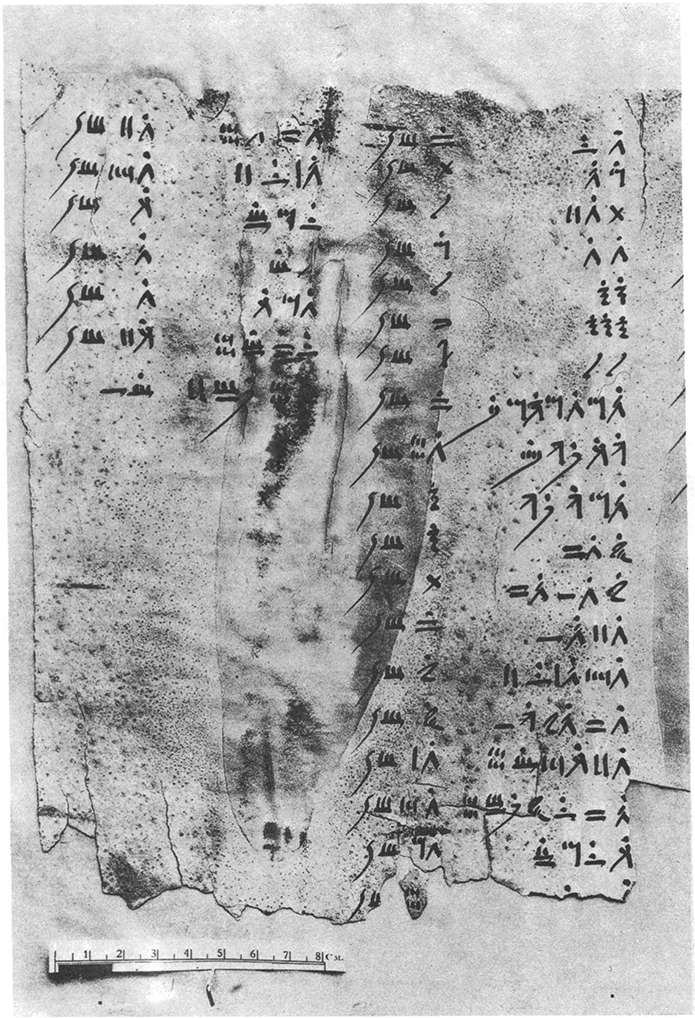
\includegraphics[width=\textwidth]{gfx/EMLR}
  \caption[Photograph of columns 3 and 4 of the Egyptian Mathematical Leather Roll.]
  {Photograph of columns 3 (right) and 4 (left) of the Egyptian Mathematical Leather Roll. Columns 3 and 4 are duplicates of columns 1 and 2. For example, row 9 of column 3 translates to $\displaystyle \frac{1}{50}\frac{1}{30}\frac{1}{150}\frac{1}{400} \quad\quad \frac{1}{16}$ in modern fraction notation where addition is implied. Figure \ref{fig:EMLRschematic} is a schematic of the table photographed here. Figure from \citet{Glanville27} which is accompanied by a translation of the hieroglyphics.}
  \label{fig:EMLR}
\end{figure}

\begin{figure}
  \centering
  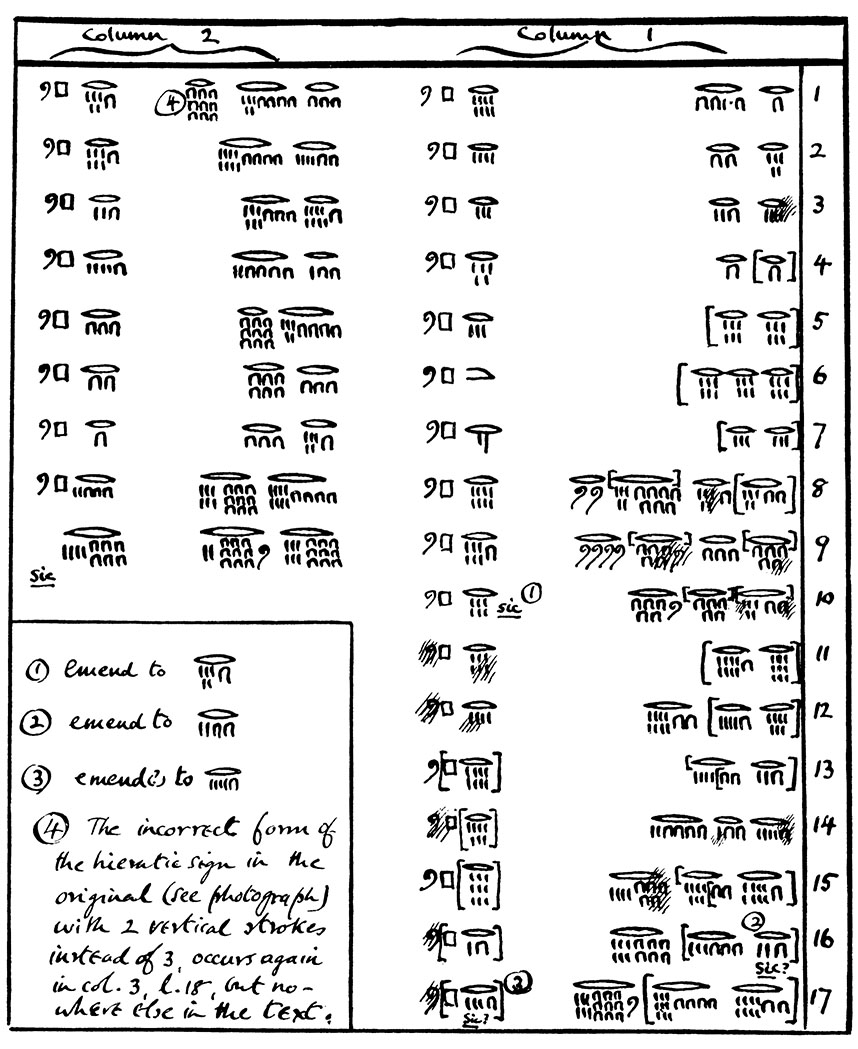
\includegraphics[width=\textwidth]{gfx/EMLRschematic}
  \caption[Schematic of columns 1 and 2 of the Egyptian Mathematical Leather Roll.]
  {Schematic of columns 1 and 2 of the Egyptian Mathematical Leather Roll. Columns 3 and 4 are duplicates of columns 1 and 2. For example, row 1 of column 1 translates to $\displaystyle \frac{1}{10}\frac{1}{40} \quad\quad \frac{1}{8}$ in modern fraction notation where addition is implied. Figure \ref{fig:EMLR} is a photograph of the table outlined here. From \citet{Glanville27} which is accompanied by a translation of the hieroglyphics.}
  \label{fig:EMLRschematic}
\end{figure}

% Of course since then lookup tables have found an enormous number of uses in computer science. Arrays are ubiquitous objects in procedural programming languages and so is the more general dictionary object, especially in Python. Sine tables are still stored in calculators for quick trigonometric computations using the CORDIC algorithm and 3D lookup tables are used in image processing to store colormaps. In each case the speed offered by a lookup table once it has been generated is the main reason for their use.

\section{Previous attempt using the Nelder-Mead method} \label{sec:nelderMead}
\index{Simplex algorithm}
\index{Geometry reconstruction!Simplex algorithm}
\citet{Brichta09} proposed the reconstruction of small triatomic molecules using a ``simplex'' algorithm. It should not be confused with the much better known simplex algorithm by George Dantzig, also an optimization algorithm but for linear programming, taught in almost every introductory optimization course. The algorithm employed should really should be referred to as the Nelder-Mead method, downhill simplex method, or amoeba method to avoid confusion between the two.\footnotemark

\footnotetext{We refer to it as the Nelder-Mead method for this chapter, as Wikipedia does. It seems that Dantzig's simplex algorithm finds more use in fields such as optimization, operations research, and economics while the Nelder-Mead simplex method has been historically popular in science and engineering due to it's ability to run on microcomputers.}

The Nelder-Mead algorithm is an ad-hoc or heuristic algorithm for nonlinear optimization that can be used without computing derivatives of the objective function\footnotemark. It was first generalized to minimizing functions by \citet{Nelder65} based off ideas by \citet{Spendley62}. It has enjoyed widespread popularity due to its ease of implementation and intuitive inner workings but it is not appropriate to every problem. In fact, it is not guaranteed to converge except for strictly convex problems in 1 and 2-dimensions \citep{Lagarias98} and thus fails when applied to some problems. It can even converge to non-stationary points in some cases \citep{McKinnon98}. Later publications would sometimes introduce modifications to the Nelder-Mead method that would improve its performance on a specific problem \citet{Wright10}. Unfortunately, I believe geometry reconstruction is not an appropriate problem for the Nelder-Mead method as we will very soon see in section \ref{ssec:simplexFail}.

\footnotetext{\citet{Wright10} provides a great discussion of the Nelder-Mead method, ending with a comment by John Nelder regarding his algorithm, ``Mathematicians hate it because you can’t prove convergence; engineers seem to love it because it often works.'' \citet[section 10.4]{NumericalRecipes} describes the algorithm in detail and provides a well-commented C++ implementation.}

\subsection{Previous reconstructions}
Unfortunately, \citet{Brichta09} only report on the reconstruction of molecular structures based on a few simulated geometries for carbon dioxide (\ch{CO2}) and formaldehyde (\ch{CH2O}). In an earlier work, \citet{Brichta07} claim to have used this algorithm to report on reconstructions of real \ch{CO2} geometries (see figure \ref{fig:simplexJPhysB}), which seems ripe for discussion and investigation, however the experimental data is not discussed and instead the focus is placed on reconstructing simulated data. It was also used by \citet{Bocharova11} to report on the molecular structure of \ch{CO2} $(2,2,2)$ (see figure \ref{fig:simplexPRL}) however both works do not report the set of geometries used to form the initial simplex. While they both produce a nice and intuitive plots, showing what appears to be an approximation to a molecular wavefunction with two broad position distributions, we will later see that such plots may appear deceptive and may not represent the reconstruction of physical geometries.

\begin{figure}
  \centering
  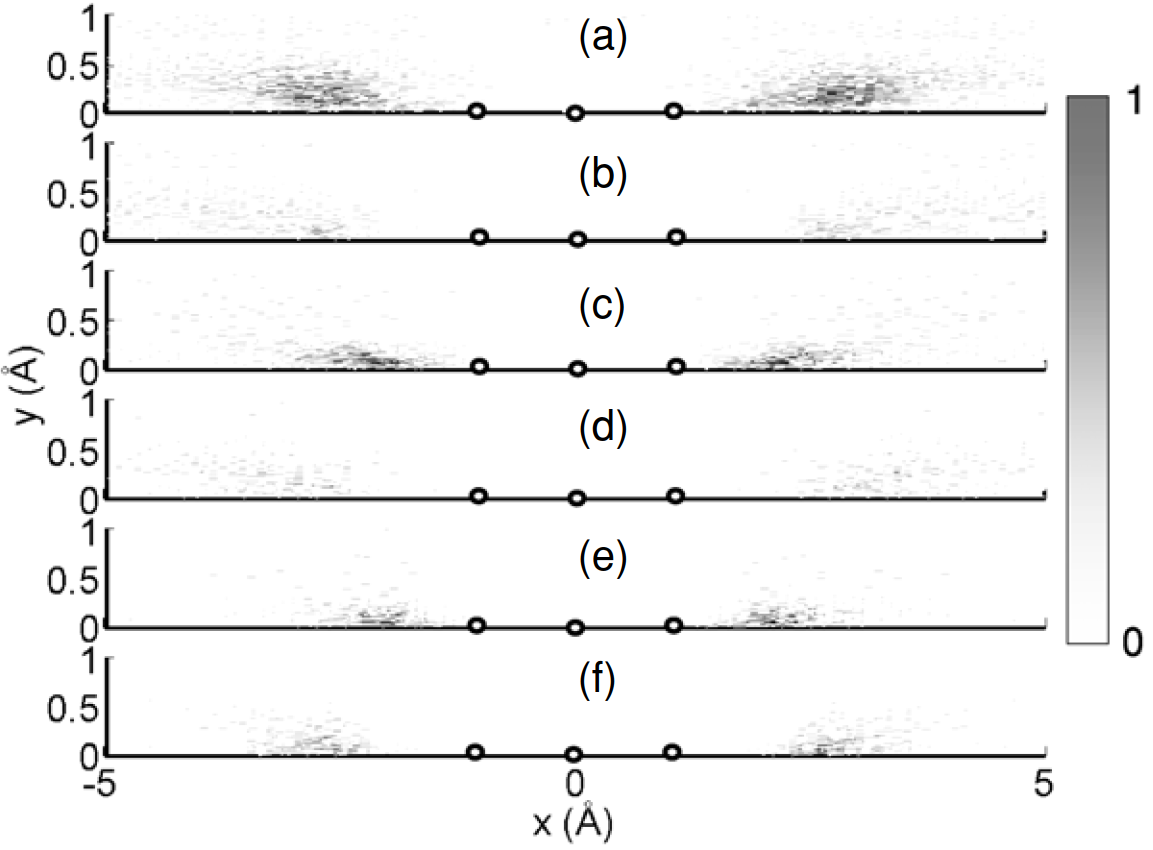
\includegraphics[width=\textwidth]{gfx/SimplexJPhysB}
  \caption[Reconstructed \ch{CO2} geometries using the Nelder-Mead simplex method.]
  {Reconstructed \ch{CO2} geometries after Coulomb explosion by \SI{50}{\fs} laser pulses using the Nelder-Mead simplex method for the (a) $(1,1,1)$, (b) $(1,2,1)$, (c) $(1,1,2)$, (d) $(1,2,2)$, (e) $(2,1,2)$, and (f) $(2,2,2)$ fragmentation channels. The carbon atom is placed at the origin with the higher charged oxygen atom in the +$x$-quadrant. A $2$D histogram is used to plot the spatial distribution of the two terminal oxygen atoms with darker colors indicating a higher count rate. The histogram is normalized such that the maximum count rate is $1$. The three circles represent the equilibrium or ground state geometry of \ch{CO2}, which is plotted as perfectly linear even though it should have a bond angle of \SI{172.5}{\degree} \citep{Siegmann02, Mathur92}. Each plot is reported to contain approximately $10^3$ events (or geometries), however (a) and (d) appear to contain quite different amounts of data. Figure from \citet{Brichta07}.}
  \label{fig:simplexJPhysB}
\end{figure}

\begin{figure}
  \centering
  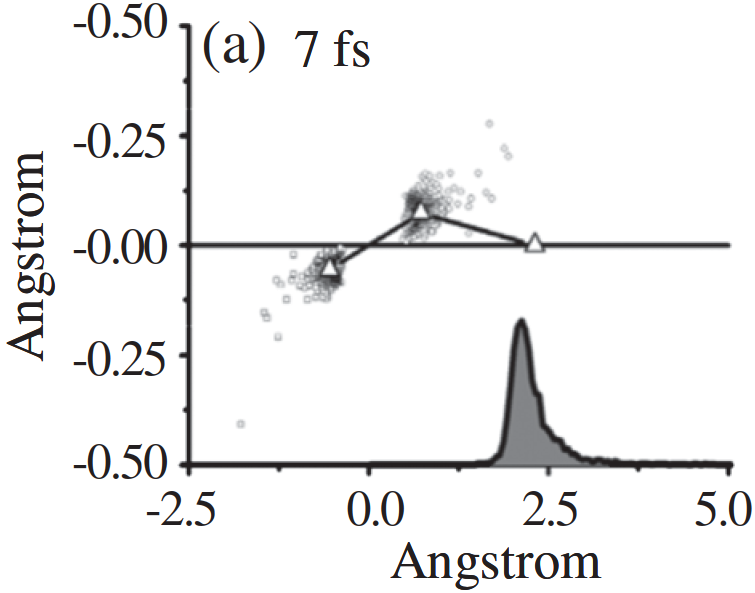
\includegraphics[width=0.6\textwidth]{gfx/SimplexPRL}
  \caption[Reconstructed \ch{CO2} in the $(2,2,2)$ charge state using the Nelder-Mead simplex method.]
  {Reconstructed \ch{CO2} geometries in the $(2,2,2)$ charge state after explosion by a \SI{7}{\fs} laser pulse using the Nelder-Mead simplex method. The oxygen in the $x>0$ plane is restricted to the $x$-axis with a probability density curve showing its distribution in space, presumably calculated using a kernel density estimate, although unreported. The circles pinpoint the location of the carbon atom and the oxygen atom in the $x<0$ plane relative to the fixed oxygen atom and the triangles presumably pinpoint the centroid (or average) position of each atom. They report a molecular geometry of $\langle r_\mathrm{CO} \rangle \approx \SI{1.3}{\angstrom}$, $\langle \theta_\mathrm{OCO} \rangle \approx 168\degree$ which is close the equilibrium geometry of $\langle r_\mathrm{CO} \rangle \approx \SI{1.16}{\angstrom}$ \citep{ChemistryOfTheElements} and $\langle \theta_\mathrm{OCO} \rangle \approx \SI{172}{\degree}$ \citep{Siegmann02, Mathur92}. Figure from \citet{Bocharova11}.}
  \label{fig:simplexPRL}
\end{figure}

\subsection{Inability to reliably reconstruct molecules} \label{ssec:simplexFail}

When we initially attempted to apply the Nelder-Mead simplex method to the problem of geometry reconstruction ourselves, we found the results to vary greatly depending on the set of geometries chosen to form the initial simplex, required by the algorithm as an input parameter, similar to an initial guess. The majority of reconstructed geometries did not make physical sense, such as having one bond length be several times longer than the other. To investigate this worrying aspect of the algorithm, we decided to see whether it could reconstruct simulated geometries. That is, we would chose a molecular geometry and use it to simulate a Coulomb explosion (see section \ref{sec:simulating}) and compute the resulting asymptotic momentum vectors. These momentum vectors are then fed into the Nelder-Mead algorithm to see whether it could recover the molecular geometry we initially picked.

Simulated geometries are used for this analysis mainly because we can check exactly how far off the algorithm is from the correct solution. The simulated geometry only experiences the Coulomb force and so at least one solution is guaranteed to exist by our deterministic classical simulation as no quantum mechanical effects occur. Simulated geometries are thus the easiest geometries to reconstruct and serious doubts regarding an algorithm's utility must be raised if it cannot reconstruct them. When dealing with experimentally measured data, we do not know the geometries \textit{a priori} and so we need a trustworthy reconstruction algorithm in order to trust any of the results it produces.

What we found confirmed the unreliable nature of the Nelder-Mead method for reconstructing molecular geometries. We attempted to reconstruct molecular structures for \ch{CO2} and \ch{OCS}, both in the $(2,2,2)$ fragmentation channel. Starting from their equilibrium geometries we varied one parameter at a time to test whether the Nelder-Mead method could recover the geometry. Figure \ref{fig:CO2SimplexCalibrationPlots} shows the reconstruction results for \ch{CO2} $(2,2,2)$ and figure \ref{fig:OCSSimplexCalibrationPlots} shows them for \ch{OCS} $(2,2,2)$. We take the ground state geometry of \ch{CO2} to be $r_\mathrm{CO} = \SI{1.16}{\angstrom}$ \citep{ChemistryOfTheElements} and $\theta_\mathrm{OCO} = \SI{172}{\degree}$ \citep{Siegmann02, Mathur92}. For \ch{OCS}, we take the ground state geometry to be $r_\mathrm{CO} = \SI{1.1578}{\angstrom}$, $r_\mathrm{CS} = \SI{1.5601}{\angstrom}$ \citep{CRCHandbook88ed}, and $\theta_\mathrm{OCS} = \SI{175}{\degree}$ \citep{Wales12HCI}.

\begin{figure}
  \centering
  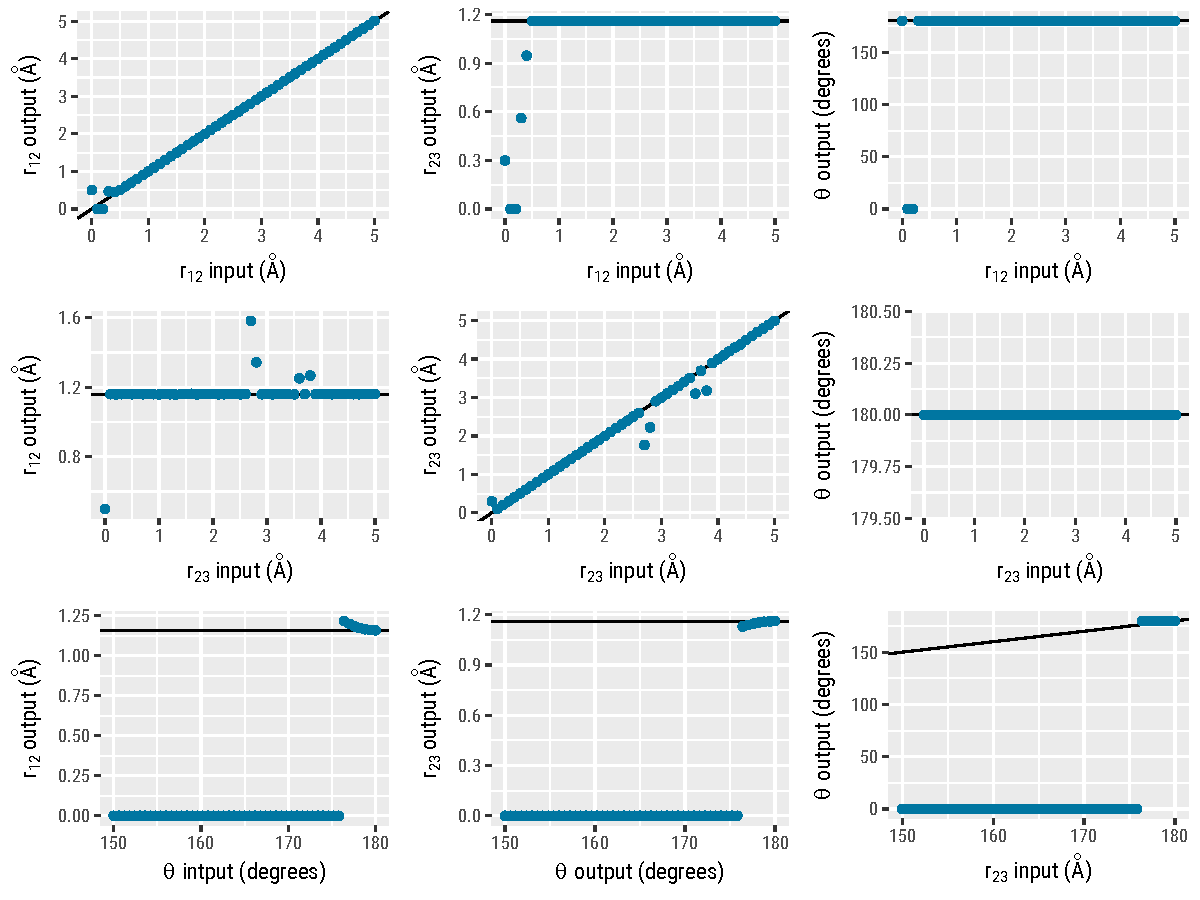
\includegraphics[width=\textwidth]{Plots/CO2SimplexCalibrationPlots}
  \caption[Testing the Nelder-Mead method's ability to reconstruct \ch{CO2} (2,2,2) geometries]
  {Testing the Nelder-Mead method's ability to reconstruct \ch{CO2} geometries in the (2,2,2) fragmentation channel by starting with the ground-state geometry of \ch{CO2} and varying each parameter one-by-one. In the first row, the first \ch{C-O} bond length ($r_{12}$) was varied to create an ``input geometry'' which underwent a simulated Coulomb explosion. The resulting momentum vectors from the explosion were fed into the Nelder-Mead algorithm which converged to a geometry, the ``output geometry''. The second \ch{C-O} bond length ($r_{23}$) and the bond angle $\theta$ were varied in the second and third rows respectively. Solid black lines indicate the expected output geometry, so deviations indicate a failure on the algorithm's ability to reconstruct the geometry. We see that the algorithm can accurately reconstruct the geometry when a single bond length is varied but completely fails once the bond angle is below approximately $176\degree$, thus simply producing zeros.}
  \label{fig:CO2SimplexCalibrationPlots}
\end{figure}

\begin{figure}
  \centering
  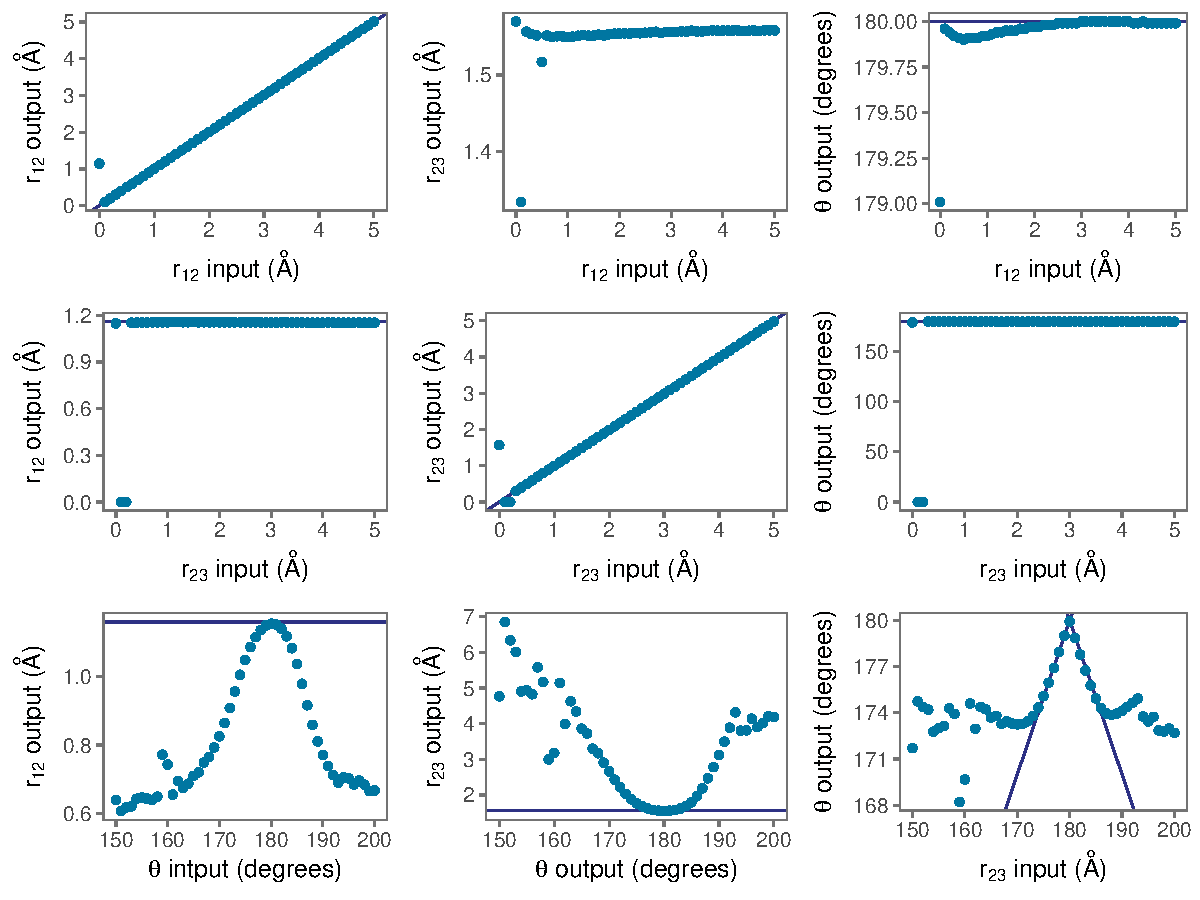
\includegraphics[width=\textwidth]{Plots/OCSSimplexCalibrationPlots}
  \caption[Testing the Nelder-Mead method's ability to reconstruct \ch{OCS} (2,2,2) geometries.]
  {Testing the Nelder-Mead method's ability to reconstruct \ch{OCS} (2,2,2) geometries by starting with the ground-state geometry of \ch{CO2} and varying each parameter one-by-one. In the first row, the \ch{C-O} bond length ($r_\textrm{CO}\equiv r_{12}$) was varied to create an ``input geometry'' which underwent a simulated Coulomb explosion. The resulting momentum vectors from the explosion were fed into the Nelder-Mead algorithm which converged to a geometry, the ``output geometry''. The \ch{C-S} bond length ($r_\textrm{CS}\equiv r_{23}$) and the bond angle $\theta$ were varied in the second and third rows respectively. Solid black lines indicate the expected output geometry, so deviations indicate a failure on the algorithm's ability to reconstruct the geometry. We see that the algorithm can accurately reconstruct the geometry when a single bond length is varied but performs worse and worse as the molecule bends, even slightly.}
  \label{fig:OCSSimplexCalibrationPlots}
\end{figure}

The Nelder-Mead method successfully retrieves the bond lengths for the majority of cases but not the bond angles. In the case of \ch{CO2} it seems to completely fail at retrieving the geometry once the bond angle falls below approximately $176\degree$. For \ch{OCS}, retrieved geometries get worse and worse as the molecule bends, even slightly.

A more thorough analysis should vary multiple parameters at once to more fully explore the state space of the problem, however if the algorithm cannot even reconstruct geometries that different from the equilibrium state by a single parameter as we have done, then the results of a more thorough analysis will probably be even more worrying. We already have enough information to distrust the Nelder-Mead method and begin searching for a new approach.

It should be noted that the Nelder-Mead algorithm, especially in our case, is quite sensitive to the geometries chosen to represent the initial simplex. Changing them could significantly impact the algorithm's ability to converge on the correct geometry. Of course, this does suggest that there may exist a set of initial geometries that significantly improve the algorithm's reliability, however, after many attempts I could not find such a set. Some choices improved the recovery of bond angles at the cost of failing to recover the correct bond lengths. The initial simplex used to produce figures \ref{fig:CO2SimplexCalibrationPlots} and \ref{fig:OCSSimplexCalibrationPlots} was chosen to maximize the number of successful reconstructions for very straight molecules which constitute the majority of cases, however molecules with bond angles $\theta < 175\degree$ are still very common and so even with this choice, we are very unsure about the accuracy of the majority of reconstructions.

% TODO: Include my initial simplex.

Perhaps \citet{Brichta07} and \citet{Bocharova11} happened to find an optimal set of geometries to form their initial simplex used to produce figures \ref{fig:simplexJPhysB} and \ref{fig:simplexPRL}, however no mention of it is made anywhere, and thus we are unable to replicate their results. The necessity and difficulty of fine tuning required should cast some doubt over their geometry reconstructions and any consequent conclusions in their respective works.

\section{Implementation}
\index{Lookup table}
\index{Geometry reconstruction!Lookup table}
The idea behind using a lookup table is quite simple: many Coulomb explosions are simulated (see section \ref{sec:simulating}) using a wide variety of molecular structures as the initial condition, and the resulting momentum vectors from each simulation are stored. This creates a mapping from molecular structures to momentum vectors. Thus by storing the results from many simulations, we end up with a lookup table. To determine the structure belonging to a certain set of observed momentum vectors, you simply read the table in reverse and search for the momentum vectors that most closely match the observed set.

In our case, we quantify this through the use of the $\ell^2$-norm squared between the sets of vectors
\begin{equation}
\left\|\mathbf{p} - \mathbf{p}'\right\|_2^2
= \sum\limits_{i = 1}^{3N} (p_i - p_i')^2
\end{equation}
for an $N$-atom molecule and where $i$ sums over each momentum component for each atom, \eg $O_x, O_y, \dots, S_y, S_z$ for the \ch{OCS} molecule. We may sometimes refer to as the \emph{objective function} and its value as the \emph{absolute error}.

% TODO: Why the L^2-norm squared?

Each molecular geometry and its corresponding post-explosion momentum vectors can be stored in a single row consisting of $9$ entries, $3$ to describe the molecular geometry of a triatomic molecule and $6$ to describe the momentum vectors. While only $3$ scalars are enough to describe the momentum vectors produced by a simulated Coulomb explosion (the last momentum vector can be calculated from the others using conservation of momentum, see section \ref{sec:conventions}), we store all $6$. This is to allow for comparison with real momentum data where throwing out some component measurements may skew the reconstruction, especially if these specific components happened to carry a large uncertainty. We are a little unsure of the consequences of only using a subset of our measurements and so we feel uncomfortable doing it.

A technical detail that is important to mention is the reason for storing and using bond lengths in units of picometers and bond angles in degrees. The bond lengths and angles differ numerically by approximately 12 orders of magnitude in SI units and so this was done to keep the parameters all on the same order of magnitude, mainly to avoid potential numerical instabilities and to make data analysis and plotting more convenient. This becomes especially important for the optimization approach we take in chapter \ref{ch:optimization} where derivatives and Jacobian matrices need to be calculated. Equivalently, we could have chosen angstroms (\SI{}{\angstrom}) and radians.

A quick, naive argument in favor of the lookup table would suggest that this approach is simple to implement, fast, and precise as the expensive task of simulating many geometries is done only once then stored. Searching through the lookup table to find a match takes linear time $\mathcal{O}(n)$ where $n$ is the number of table entries,\footnotemark~ and the precision is set when simulating the many geometries ($\SI{0.05}{\angstrom}$ and $\SI{0.25}{\angstrom}$ in our case). However, one major problem we will see in section \ref{ssec:LTspace} is that the space requirements scale worse than exponentially with the size of the molecule and precision required. Even worse, this approach assumes that the true geometry is in the vicinity of the geometry found using the lookup table. This is equivalent to assuming that every local minimum is a global minimum (or that this is a convex optimization problem), which we will find out is not true. One important and interesting exception is the presence of degenerate geometries (section \ref{ssec:degenerateGeometries}) and later, saddle points that increase exponentially in number with the dimension of the problem ($3N-6$ for a molecule with $N$ atoms).

\footnotetext{It takes linear time because we must search through every single entry before concluding that we have found the best match. If we could sort our entries in some way then we could perform a binary search instead taking logarithmic time $\mathcal{O}(\log n)$ however that would require distilling each entry to an appropriate scalar, which would differ for each geometry and take linear time to perform anyway.}

For these reasons, the lookup table was abandoned rather quickly in favor of a mathematical optimization approach that requires no results to be stored, and is aware of the presence of degenerate solutions. But before abandoning it, it is worth analyzing its disadvantages in some detail to explore the nature of the problem of reconstructing geometries. It may have some future usefulness too and we discuss some potential applications.

\subsection{Computational space complexity} \label{ssec:LTspace}

One of the disadvantages of using a lookup table for this particular problem is the amount of storage space it occupies.  As a concrete example, our lookup table for \ch{OCS} contained geometries spanning a cube in phase space ($\SI{0.50}{\angstrom} \le r_\mathrm{CO}, r_\mathrm{CS} \le \SI{5.00}{\angstrom}$, $\SI{140}{\degree} \le \theta_\mathrm{OCS} \le \SI{180}{\angstrom}$) that we believe should contain all physically realizable geometries. Individual geometries spanned the discrete ranges $r_\mathrm{CO}, r_\mathrm{CS} \in [0.50, 0.55, \dots, 4.95, 5.00] \SI{}{\angstrom}$ and $\theta_\mathrm{OCS} \in [140.00\degree$, $140.25\degree$, $\dots$, $179.75\degree$, $180.00\degree]$ giving a precision of \SI{0.05}{\angstrom} for the bond lengths and \SI{0.25}{\degree} for the bond angle. This gives us a lookup table with $91 \times 91 \times 161 = 1,333,241$ entries. Since each entry contains $9$ 64-bit floating-point numbers, it requires $9 \times \SI{8}{\byte} = \SI{72}{\byte}$ to store each entry.\footnotemark~ To store the entire table, that is $1,333,241 \times \SI{72}{\byte} = \SI{95.993}{\mega\byte}$. Such a table, if stored in human-readable ASCII such as in a comma-separated value file would take up more space ($\SI{262}{\mega\byte}$) but can be compressed efficiently ($\SI{24}{\mega\byte}$ using 7-zip).

\footnotetext{There are $8$ bits in a byte (\SI{}{\byte}) so a single $64$-bit float would take $8$ bytes to store. MATLAB uses $64$-bit double precision floating point numbers by default but other programming languages may use single precision $32$-bit floating point numbers by default, even when running on a $64$-bit processor.}

Let us calculate the size of a higher resolution lookup table and a lookup table for a 4-atom molecule. For a molecule with $N$ atoms, each entry would require $3N-6$ entries to describe the geometry and $3N-3$ to describe the momentum vectors for a total of $6N-9$ entries per geometry. If $d_i$ denotes the number of values simulated for parameter $i$ (\eg $d_1 = 91$, $d_2 = 91$, and $d_3 = 161$ for our lookup table) then the total number of entries will be $\displaystyle \prod\limits_{i=1}^{3N-6} d_i$, or simply $d^{3N-6}$ if $d_i = d$ for all $i$ so that we use the same number of simulated values for each parameter. Thus the total storage space used up by such a lookup table, in bytes, is
\begin{equation}
8(6N-9)d^{3N-6}\sim \mathcal{O}(Nd^{N})
\end{equation}
which increases exponentially with an increase in the number of atoms $N$ and follows a power law in the number of simulated values $d$ per parameter. The number of simulated values $d$ required to achieve a certain precision $\epsilon < 1$ is $d = (p_\mathrm{max} - p_\mathrm{min})/\epsilon$ where $[p_\mathrm{min}, p_\mathrm{max}]$ is the range of possible parameter values we wish to simulate, and so the size of the lookup explodes very quickly with increased precision requirements ($\epsilon \rightarrow 0$) as well.

For example, a lookup table that is five times more precise than ours ($\epsilon_r = \SI{0.01}{\angstrom}$ and $d_r = 451$ for bond lengths, $\epsilon_\theta = \SI{0.05}{\degree}$ and $d_\theta = 801$ for bond angles) takes up $\SI{8}{\byte} \times 9 \times 451^2 \times 801 = \SI{11.7}{\giga\byte}$ of storage space, or $122 \approx 5^3$ times more space. Storing such a table in memory, and thus searching speed which used to only take linear time, starts to become a major concern. Going up to a larger $4$-atom molecule such as acetylene and using the same coarse precision as our lookup table did ($\epsilon_r = \SI{0.05}{\angstrom}$ and $d_r = 91$ for bond lengths, $\epsilon_\theta = \SI{0.25}{\degree}$ and $d_\theta = 161$ for bond angles), a lookup table would take up $\SI{8}{\byte} \times 15 \times 91^3 \times 161^3 = \SI{377}{\tera\byte}$ or almost 4 million times larger, now requiring a distributed database management system; completely overkill to solve a relatively simple problem. It seems that this lookup table approach will not scale at all to larger molecules without massive sacrifices in precision. Plus, using gigabytes to store a lookup table seems like a huge waste and suggests we must seriously look for a method that does not require large amounts of data to reconstruct geometries.

\subsection{Zooming in for more precise reconstructions}

Another immediate disadvantage of such an approach is that you are limited to recovering only the geometries that are included in the table. One way to increase the precision of the lookup table approach without using up additional storage space is to use the table as a coarse first-order approximation. Once a geometry is found using the lookup table, you can dynamically simulate many similar geometries (neighbouring geometries in phase space) on-the-fly which can then be searched for a more precise match. This can be applied iteratively, reducing the volume of phase space searched at each iteration, until a desired precision is reached.

In our case, we chose to increase the precision by a factor of $5$ each iteration so that we search through a cube in phase space with a volume that is $5^3$ times smaller each iteration (in an attempt to precisely locate the local minimum). Each iteration we simulate geometries with $10$ values for each parameter, so $10^3$ geometries in total. We stop after $5$ iterations or after a desired error threshold is reached. Typically an error of $10^{-48}$ gives 1-2 significant figures of precision while an error of $10^{-50}$ gives 2-3 significant figures. This step can be computationally expensive, requiring the additional simulation of thousands of geometries per geometry recovered, however a single simulation takes on the order of $\SI{10}{\ms}$ to complete on a personal laptop so it will complete in a reasonable timeframe and this lets us arbitrarily increase the precision of our reconstruction without using up an exorbitant amount of storage space. It does feel quite wasteful though as it seems that the entire field of mathematical optimization attempts to solve this very problem of finding minima.

One possible improvement is to store these thousands of extra simulations as extra lookup table rows, effectively extending the lookup table. This storing or caching of the results of expensive function calls is termed \emph{memoization}. It may help if the geometries being reconstructed tend to lie close to each other, however in practice the sparsity of reconstructed geometries relative to the resolution of these extra rows results in almost no improvements in performance.

\subsection{Using simulations to test accuracy} \label{ssec:LTaccuracy}
Since we used simulations to test the accuracy of the Nelder-Mead simplex method in section \ref{ssec:simplexFail}, it is only fair that we subject the lookup table to the same analysis.

% TODO: Find or recreate these plots!

It is important that we do not simulate geometries that are already contained in the lookup table otherwise the reconstruction is trivial.

\section{Geometry reconstructions done by lookup table} \label{sec:LTgeometries}

With the knowledge that the lookup table can be somewhat trusted, we should use it to reconstruct some real geometries. Here we will reconstruct the  \ch{OCS} $(2,2,2)$ geometry. Figure \ref{fig:OCS2227fsLTGeometry} shows one such geometry, forming the first frame of a molecular movie.

\begin{figure}
  \centering
  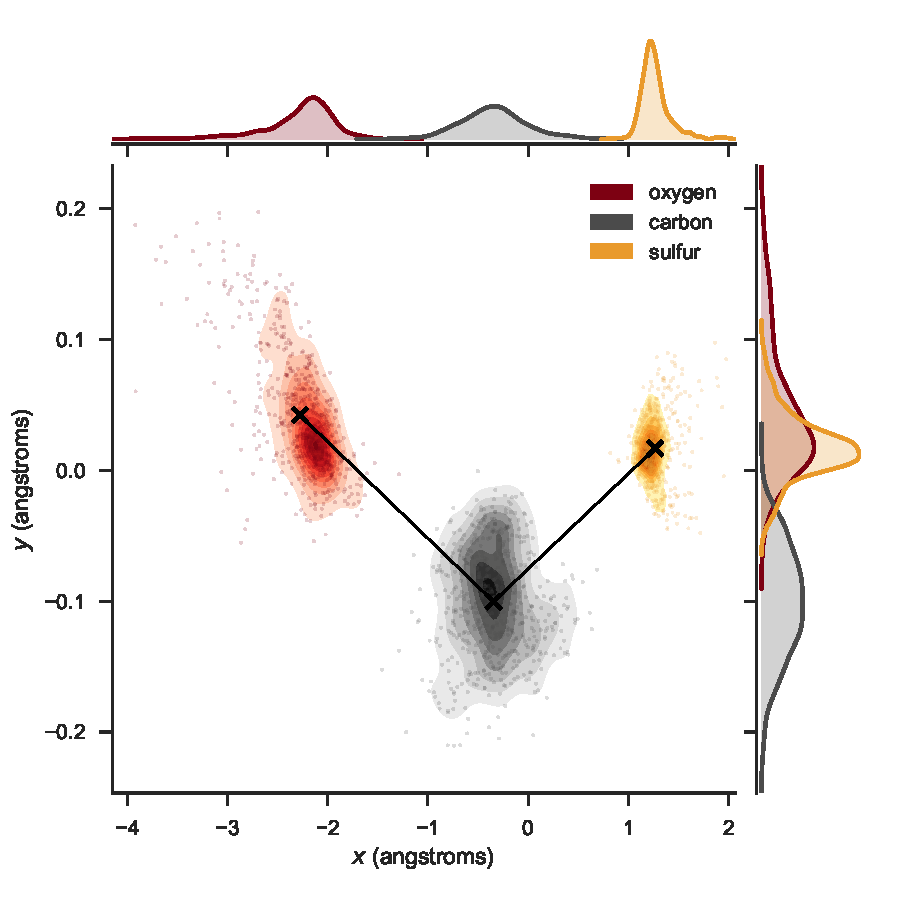
\includegraphics[width=\textwidth]{Plots/OCS2227fsLTGeometry}
  \caption[Scatter plot showing the molecular geometry of \ch{OCS} following Coulomb explosion by a \SI{7}{\fs} laser pulse for the $(2,2,2)$ fragmentation channel.]
  {Scatter plot showing the molecular geometry of \ch{OCS} following Coulomb explosion by a \SI{7}{\fs} laser pulse for the $(2,2,2)$ fragmentation channel. Each geometry is represented by three colored points, one for each atomic fragment; red for oxygen on the left, black for carbon in the center, and yellow for sulfur on the right. The colors were chosen to imitate the CPK coloring convention. Geometries are plotted such that the molecule's center of mass is at the origin to showcase the variance in each atomic fragment's position, and are rotated such that a vertical line bisects the \ch{O-C-S} bond angle. Bivariate kernel density estimates (with a Gaussian kernel), plotted as shaded-in contours, are used to estimate the the probability density of each atomic fragment's position. Solid black lines are drawn between the peaks of each atomic fragment's kernel density estimate to illustrate the \emph{modal geometry} or most likely geometry. Along the top of the plot, marginal distributions show the probability density of each atomic fragment's position along the $x$-axis and the same is done for the $y$-axis along the right. The modal geometry is calculated to be $r_\mathrm{CO} = \SI{1.32}{\angstrom}$, $r_\mathrm{CS} = \SI{1.26}{\angstrom}$, $ \theta_\mathrm{OCS} = 172.7\degree$ while the average geometry of $r_\mathrm{CO} = \SI{1.39}{\angstrom}$, $r_\mathrm{CS} = \SI{1.27}{\angstrom}$, $ \theta_\mathrm{OCS} = 171.6\degree$ is slightly larger due to outliers. The molecule is almost straight but an aspect ratio of approximately $12:1$ is employed to showcase variability in the $y$-axis. In chapter \ref{ch:optimization} we will see that plotting geometries in this manner, while intuitive and satisfying, can be misleading.}
  \label{fig:OCS2227fsLTGeometry}
\end{figure}

Here we have plotted the geometries by placing the center of mass at the origin, giving us three probability distributions, one for each atomic fragment which allows us to see the variance in each atomic fragment's position. We could have placed the carbon at the center resulting in just two distributions, one for each of the terminal atoms much like \citet{Brichta07} did in figure \ref{fig:simplexJPhysB} however we felt that this approach provides less information. \cite{Bocharova11}, in figure \ref{fig:simplexPRL}, plot the geometries with a terminal oxygen at a fixed position along the $x$-axis and include a one-dimensional marginal distribution of the oxygen's position along the $x$-axis, which is an improvement but we feel that it still provides less information.  We use the same visualization method as \citet{Legare05structure} (see figure \ref{fig:SO2-232structure}) who revert to a plot like the one by \citet{Bocharova11} in their later work for reasons unknown \citep{Legare05dynamics}.

An argument could be made for each visualization method, however in the end it probably does not matter how the geometries are plotted. In chapter \ref{ch:optimization} we will see that plotting geometries in this manner alone, while intuitive and satisfying, can be very misleading in that it can be used to hide unphysical data and make it appear agreeable. This is because the ensemble of geometries reconstructed seems to make physical sense while most of the individual geometries reconstructed do not upon further inspection. We do not know much about the individual geometries from such a plot as we do not know which points are correlated with which.

% TODO: Any explanation for this?
The calculated modal and average geometries may appear quite worrying as they suggest a stretching of the \ch{C-O} bond and a compression of the \ch{C-S} bond. % Now, I'm not saying they're right or wrong, just that I don't trust them.

A critical issue worth investigating is quantifying how much uncertainty there is in these molecular geometries. This is a complicated problem we will tackle in chapter \ref{ch:uncertainty}.

We can repeat this analysis for the other laser pulse widths (\SIlist{30;60;100;200}{\fs}). In table \ref{table:lookupTableSuccess} we tabulate the number of geometries we were able to successfully reconstruct, which decreases as the pulse length increases indicating a greater difficulty in reconstructing geometries. The longer the laser pulse, the more time the molecule has to distort its structure in response to the laser's intense electric field, reducing the validity of the assumption that the molecule evolves along a purely classical Coulomb potential.

To conserve space, the geometry reconstructions for Coulomb explosion by \SIlist{30;60;100;200}{\fs} laser pulses are provided in appendix \ref{appx:supplementaryFigures}, figures \ref{fig:OCS22230fsLTGeometry}--\ref{fig:OCS222200fsLTGeometry}.

\begin{table}
  \myfloatalign
  \centering
  \begin{tabularx}{0.875\textwidth}{cccc}
    \toprule
    Pulse width (\SI{}{\fs}) & Geometries & Reconstructions & Success \\
    \midrule
    7 & 795 & 584 & 73\% \\
    30 & 1000 & 518 & 52\% \\
    60 & 358 & 154 & 43\% \\
    100 & 531 & 226 & 43\% \\
    200 & 500 & 190 & 38\% \\
    \bottomrule
  \end{tabularx}
  \caption[Statistics for geometry reconstruction by lookup table.]
  {Statistics for geometry reconstruction by lookup table.}
  \label{table:lookupTableSuccess}
\end{table}

Of particular interest might be the average and modal (most likely) geometries recovered, which we tabulate in table \ref{table:lookupTableGeometries}.

\begin{table}
  \myfloatalign
  \centering
  \begin{tabularx}{0.9\textwidth}{ccccccc}
    \toprule
    & \multicolumn{3}{c}{Modal geometry} & \multicolumn{3}{c}{Average geometry} \\
    Pulse width (fs) & $r_\mathrm{CO}$ & $r_\mathrm{CS}$ & $\theta_\mathrm{OCS}$ & $r_\mathrm{CO}$ & $r_\mathrm{CS}$ & $\theta_\mathrm{OCS}$ \\
    \midrule
    7 & 1.32 & 1.26 & 172.7 & 1.39 & 1.27 & 171.6 \\
    30 & 1.53 & 1.32 & 171.7 & 1.58 & 1.43 & 170.3 \\
    60 & 1.56 & 1.40 & 171.4 & 1.60 & 1.47 & 170.4 \\
    100 & 1.59 & 1.47 & 170.6 & 1.65 & 1.57 & 169.12 \\
    200 & 1.78 & 1.49 & 171.4 & 1.76 & 1.65 & 163.2 \\
    \bottomrule
  \end{tabularx}
  \caption[Average and modal geometries reconstructed using a lookup table.]
  {Average and modal geometries reconstructed using a lookup table.}
  \label{table:lookupTableGeometries}
\end{table}

% TODO: Move to ``Exploratory data analysis''?
\subsection{Kernel density estimation} \label{sec:kde}
Probability distributions for the atomic positions in the $xy$-plane and along both the $x$- and $y$-axes in figure \ref{fig:OCS2227fsLTGeometry} are estimated using kernel density estimates (KDE's) which may be thought of as a smoothed histogram that integrates to one (like a probability distribution). They are a method of performing nonparametric statistics, that is, of fitting observations to a probability distribution that has no dependency on a parameter \citep[\S 20.2-20.3]{Kendall99}. They serve roughly the same purpose as a histogram, however histograms tend to be non-smooth and their shape depends on both the width of the bins and the ends points of the bins. To solve at least the first two problems, we can use a KDE.

% TODO: Might be better than histograms, and definitely are great for higher dimensions where you get hit hard by the curse of dimensionality.

For independent and identically distributed univariate samples $x_1, x_2, \dots, x_n$ drawn from an unknown probability distribution $f$, its KDE is
\begin{equation}
\hat{f}_h(x) = \frac{1}{n} \sum_{i=1}^n K_h(x-x_i)
= \frac{1}{nh} \sum_{i=1}^n K\left(\frac{x - x_i}{h}\right)
\end{equation}
where $K$ is the \emph{kernel}, a function with zero mean that integrates to one, and $h > 0$ is the \emph{bandwidth}, a smoothing parameter analogous to the bin width \citep[p. 137]{Scott15}. Many kernel choices exist such as the rectangle or triangle function but the standard normal (or Gaussian) kernel is the most popular. Multivariate KDE's replace the scalar bandwidth parameter $h$ with a symmetric and positive bandwidth matrix $\mathbf{H}$ with a variable number of smoothing parameters \citep{Wand93} however full bandwidth matrices seem to give markedly better performance \citep{Duong03}.

Selection of the bandwidth $h$, as expected, is the most difficult aspect of KDE. Analytical formulae can be derived for the bandwidth $h$ \citep[p. 143]{Scott15} that accurately estimate the unknown density $f$ by minimizing the mean integrated squared error (MISE) however they require knowledge of the unknown density $f$ and so cannot generally be used. Fortunately, when estimating a normal (or Gaussian) density, the bandwidth that minimizes the MISE is given by \citet{Silverman86} as
\begin{equation}
  h = \left(\frac{4\hat{\sigma}^5}{3n} \right)^\frac{1}{d+4}
    \approx 1.06 \left(\frac{\sigma^5}{n} \right)^\frac{1}{d+4}
\end{equation}
where $n$ is the number of observations, $\hat{\sigma}$ is the standard deviation of the samples, and $d$ is the dimensionality of the observations (so $d=1$ for univariate observations and $d=2$ for bivariate). This is termed the \emph{normal distribution approximation} or the ``rule of thumb''. As our atomic positions seem to rougly follow a normal distribution, we used the \citet{Silverman86} rule of thumb.\footnotemark~ It is worth noting that it does not perform well on multimodal data which is why certain estimates in figure \ref{fig:OCS222100fsMomentum} appear oversmoothed.

\footnotetext{Figure \ref{fig:OCS2227fsLTGeometry} was plotted using the Python seaborn package which is built upon the SciPy and MatplotLib packages, and uses SciPy to perform the KDE. See colophon (appendix \ref{appx:colophon}) for more details.}

Other methods do exist, and univariate estimators are especially effective as briefly surveryed by \citet{Jones96}, but bandwidth selection for multivariate kernel density estimates is quite difficult for non-Gaussian densities \citep[\S 6.5.2]{Scott15}.

\section{Degenerate molecular geometries} \label{sec:degenerateGeometries}
In chapter \ref{ch:introduction} we hinted at the fact that due to the ill-posed nature of the geometry reconstruction inverse problem, multiple solutions may be posible. While investigating the reconstructed geometries, this feature surprisingly did pop up for the \ch{OCS} molecule and the lookup table can help provide some insight into these multiple solutions, which we will call \emph{degenerate geometries}.

The high precision to which we were able to recover the two degenerate geometries suggests that presence of degenerate geometries corresponds to the existence of multiple global minima. This suggests the use of a method that can locate multiple minima, which we will employ in the next chapter.

% TODO: What set of measured momentum vectors do you refer to in the figure?

\begin{figure}
  \centering
  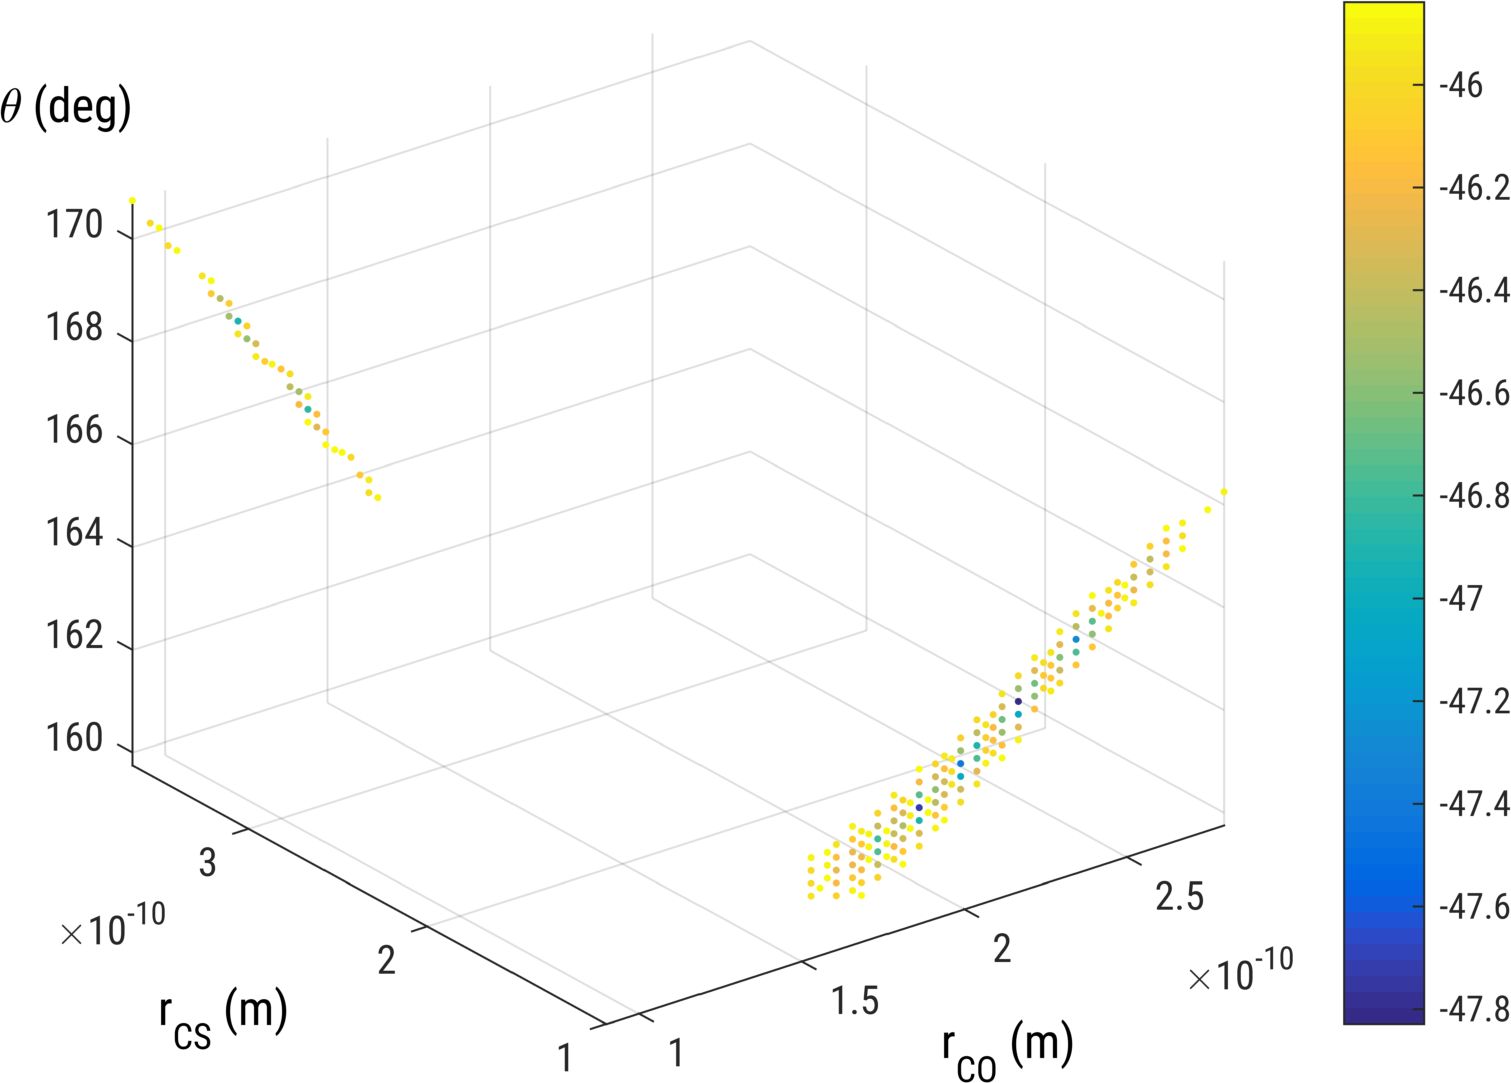
\includegraphics[width=\textwidth]{Plots/rainbow}
  \caption[3D scatter plot in phase space of the $200$ best geometries matching a particular set of measured momentum vectors, showing the existence of two degenerate geometries.]
  {3D scatter plot in phase space of the $200$ best geometries matching a particular set of measured momentum vectors, showing the existence of two degenerate geometries. Each point is colored according to the base-$10$ logarithm of the absolute error ($2$-norm) squared between the measured momentum vectors and the momentum vectors resulting from Coulomb exploding the geometry corresponding to that data point. So the darkest purple corresponds to an error of just under $10^{-47.8}$. Two disparate sets of geometries are apparent suggesting that this particular set of measured momentum vectors could have resulted from the Coulomb explosion of two very different molecular geometries, one where the \ch{C-O} bond is more stretched, and another where the \ch{C-S} bond is more stretched and the molecule is less bent. Interestingly, the points do not seem to form balls or blobs in phase space, but rather possess elongated and angled rod-like distributions. The one with the stretched \ch{C-O} bond seems to have more points but this does not suggest that this geometry is more likely. Rather, it may suggest that it is easier to converge to, or that it may have a larger \emph{basin of attraction}. We see that there are many yellow data points (relatively high error) surrounding one or two purple points (relatively low error) for each region indeed showing the low-resolution nature of our lookup table. This same information may be plotted using $2$D colormapped volumetric slices or contour slices which may even be animated to provide a visual scan through the full phase space volume. However due to the angled distribution formed by the spatial sets and the significance of only one or two data points, it becomes very difficult to visually locate the local minima even with angled slices. Another visualization method may be to use convex hulls or alpha shapes which will also allow us to assign each region a shape and volume. In figure \ref{fig:DegenerateGeometryTrajectories} we take these two degenerate geometries, Coulomb explode them, and plot their trajectories to show that even though they show slightly different dynamics, both simulations result in the exact same momentum vectors being measured.}
  \label{fig:rainbow}
\end{figure}

% TODO: What is the difference in dynamics?
\begin{figure}
  \centering
  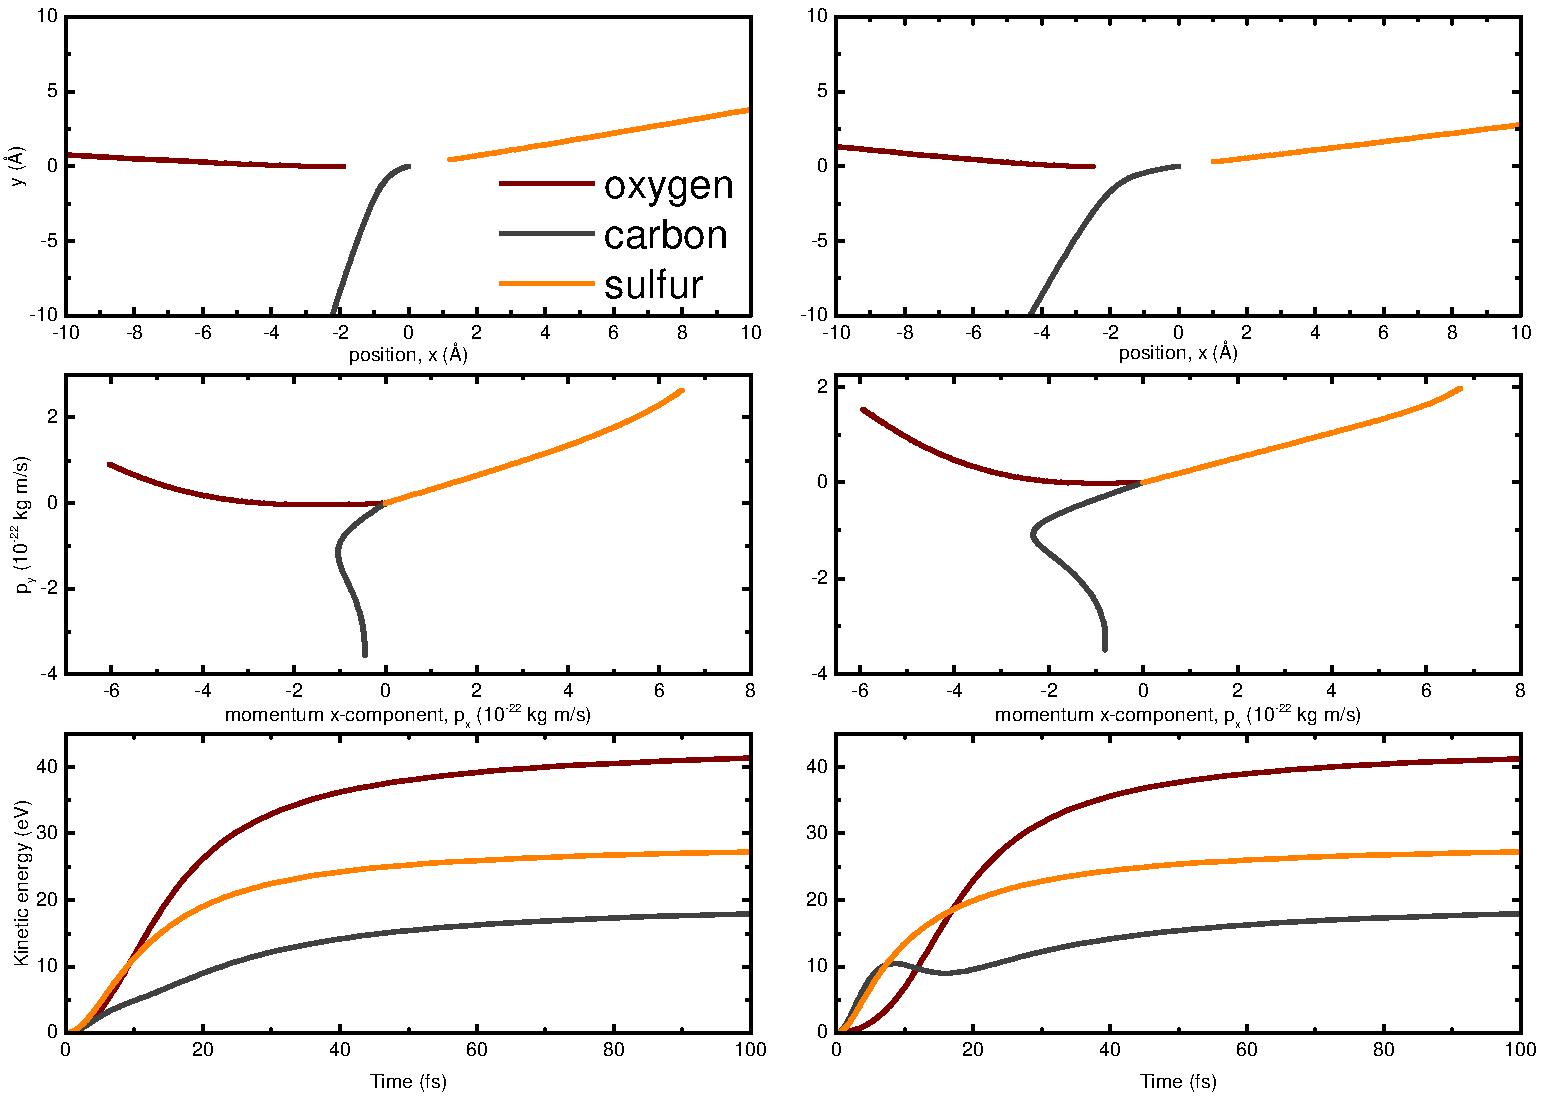
\includegraphics[width=\textwidth]{Plots/DegenerateGeometryTrajectories.pdf}
  \caption[Atomic trajectories in position and momentum-space, and kinetic energy, of two degenerate molecular geometries undergoing a Coulomb explosion.]
  {Atomic trajectories in position and momentum-space, and kinetic energy, for the oxygen, carbon, and sulfur atoms of two degenerate \ch{OCS} molecular geometries in the $(2,2,2)$ charge state undergoing a Coulomb explosion staring from rest. The plots on the left correspond to an \ch{OCS} molecule with $r_\textrm{CO} = \SI{1.8949}{\angstrom}$, $r_\textrm{CS} = \SI{1.2990}{\angstrom}$, and $\theta_\mathrm{OCO} = \SI{160.601}{\degree}$ while the plots on the right correspond to an \ch{OCS} molecule with $r_\textrm{CO} = \SI{2.486}{\angstrom}$, $r_\textrm{CS} = \SI{1.0755}{\angstrom}$, and $\theta_\mathrm{OCO} = \SI{164.568}{\degree}$. Triatomic molecules explode in a plane so their momentum vectors are only plotted in the $p_x$-$p_y$ plane although the atomic fragments will possess some momentum in the $z$-direction due to the presence of the constant electric field, it will not deviate from equation \eqref{eq:CEImomenta} and is irrelevant for these simulated Coulomb explosions. The molecular geometries are quite different yet when they undergo a Coulomb explosion, they produce the exact same set of momentum vectors once rotated into our convention (see section \ref{sec:conventions}). Well, we can make the absolute error (or $2$-norm) between the two sets of momentum vectors arbitrarily small with increased precision in describing the geometries. We see that the molecular dynamics are a little different yet in both cases, all three atoms emerge with the exact same kinetic energy. These two geometries were found by searching through the entire lookup table for the geometries best matching a particular set of measured momentum vectors (see figure \ref{fig:rainbow}). The lookup table actually does not give us enough precision to recover these geometries to several decimal places so we used the lookup table to find a measurement corresponding to two degenerate geometries, and then used the optimization method from chapter \ref{ch:optimization} to actually recover the geometries with much higher precision.}
  \label{fig:DegenerateGeometryTrajectories}
\end{figure}

\section{Conclusions}
\emph{Geometries may be reconstructed using a lookup table}---We find this approach more reliable and robust that the Nelder-Mead simplex method approach employed by \citet{Brichta09}, and it has provided us with some additional insight into the problem of reconstructing geometries especially regarding the existence of degenerate geometries. This makes the lookup table potentially useful for future investigations and reconstructions of triatomic molecules. However, the method possesses multiple flaws that leave a lot to be desired, motivating the need for another method.

\subsection{Lessons learnt}
\emph{Degenerate geometries exist}---An unexpected result of \\

\noindent
\emph{Inability to precisely reconstruct geometries}---Using just the vanilla lookup table you are limited to recovering molecular geometries contained in the lookup table. Due to storage space restrictions, the lookup table can only provide low-resolution reconstructions. \\

\noindent
\emph{Inability to differentiate between global and local minima}---The lookup table cannot choose between two degenerate geometries and due to it's low resolution it cannot distinguish between global and local minima. It may be easily modified to report on multiple solutions but doing so may be computationally expensive and begs for a more sophisticated approach. \\

\noindent
\emph{Inability to scale to larger molecules}---As discussed in section \ref{ssec:LTspace}, trying to use the lookup table to reconstruct molecules containing even as little as 4 atoms requires prohibitive amounts of storage space ($\SI{>100}{\tera\byte}$) to store the lookup table. This may be circumvented by fixing some molecular parameters if they vary very little but this trick won't get you far at all.

\subsection{Future applications}

\emph{Finding an initial or first-order solution or initial guess}---As the lookup table may quickly find coarse-grained geometries, the recovered geometry may be used as an initial guess or first-order solution for another algorithm. \\

\noindent
\emph{Visualizing the objective function for a specific set of momentum vectors}---Such a plot would assign a scalar error value to every point in phase space, allowing us to quickly visualize the objective function. This would visualize the location of degenerate geometries and provide some insight into the nature of the objective function. For example, if it is smooth and convex with a single global minimum, it would suggest that geometry reconstruction in that particular case is computationally easy. However, a jagged and discontinuous function with multiple minima and saddle points would suggest that geometry reconstruction is much more difficult. For triatomic molecules the $3$-dimensional objective function may be visualized using colormapped volumetric slices or contour slices. Unfortunately this becomes unfeasible for larger molecules due both the size of the lookup table and the difficulty of visualizing an $n$-dimensional scalar function ($n>3$). Instead of generating a lookup table, the objective function can be plotted dynamically (by simulating a Coulomb explosion at every point of interest) if the resolution is reduced. Fixing certain parameters would reduce the dimensionality of the objective function, allowing $2$-dimensional slices of it to be easily visualized. Or one could look towards methods of visualizing high-dimensional scalar functions. \\

\noindent
\emph{Finding degenerate regions of phase space quickly}---At least for triatomic molecules, where generating and storing a lookup table is feasible, it may be quickly searched to determine whether a set of measured momentum vectors correspond to just one geometry, or multiple degenerate geometries. 
\chapter{Geometry reconstruction using constrained nonlinear optimization}\label{ch:optimization}

\vspace{-1.5 em}
\begin{addmargin}[-0.5cm]{0cm}
  \minitoc
\end{addmargin}
\hrule
\vspace{1.5 em}

In the previous chapter, we saw that a lookup table approach could be used to perform geometry reconstruction using Coulomb explosion imaging. However, numerous drawbacks including the lookup table's exponential computational space complexity (severely limiting its scalability to larger molecules) and its inability to both provide precise reconstructions as well as distinguish between local and global minima leave much to be desired.

In this chapter, we will approach the task of geometry reconstruction as an optimization problem, allowing us to utilize the the much more sophisticated methods of constrained nonlinear optimization. Before we describe our reconstruction methods, it will be worthwhile to provide some background on the theoretical framework underpinning the optimization algorithms we utilize. We will then describe our implementation and use it to reconstruct the same molecular structures seen in the previous chapter, allowing for some comparison between methods and for some verification of the results. We will then further study the individual geometries recovered and the nature of the degenerate geometries seen in section \ref{sec:degenerateGeometries}, bringing to light some troubling issues regarding the problem of geometry reconstructing as well as highlighting its pathalogical nature.

\section{Mathematical optimization}
We will take a massively expedited tour of mathematical optimization with the aim of explaining the inner workings of the primal-dual interior point methods used for nonlinear constrained optimization in this chapter. To understand how these methods operate, we will need to introduce some important concepts in optimization, namely the duality principle, the Karush-Kuhn-Tucker (KKT) optimality conditions, and the general concept of a trust region. This is prefaced with a brief introduction to the subject.

No knowledge of mathematical optimization is required, however we will assume some background knowledge throughout this appendix, namely a familiarity with linear algebra, matrix algebra, vector calculus, and some elementary concepts in analysis. \citet{Boyd04} provides an excellent introduction to mathematical optimization, particularly convex optimization, and their freely-available textbook is accompanied by video lectures and lecture slides. However, our problem is nonconvex and so we turn to \citet{Nocedal06} who discuss the more advanced interior-point methods suitable for nonconvex optimization with great clarity.

\subsection{Elementary concepts} \label{ssec:elementaryOptimization}
The standard form of a (continuous) optimization problem is
\begin{align} \label{eq:op}
\mathrm{minimize}   \quad & f_0(x) \nonumber \\
\mathrm{subject\;to} \quad &
f_i(x) \leq 0, \; i \in \left\{1, \dots, m \right\}\\
& h_i(x) = 0, \; i \in \left\{1, \dots, p \right\} \nonumber
\end{align}
where $f_0(x): \mathbb{R}^n \rightarrow \mathbb{R}$ is the \emph{objective function} to be minimized over the variable $x \in \mathbb{R}^n$, $f_i(x) \leq 0$ are called the \emph{inequality constraints}, and $h_i(x) = 0$ are called the \emph{equality constraints}. We denote its domain by
\begin{equation}
\mathcal{D} = \bigcap_{i=1}^m \operatorname{dom} f_i \cap \bigcap_{i=1}^p \operatorname{dom} h_i \neq \emptyset
\end{equation}
and assume it is nonempty.

Optimization problems can be classified based on the nature of the objective function and constraints, with each class having their own algorithms. Perhaps the simplest commonly encountered class is \emph{linear programs} where the objective function and constraints are linear, that is $f_0, \dots, f_m, h_1, \dots, h_p$ all satisfy $f_i(\alpha x + \beta y) = \alpha f_i(x) + \beta f_i(y)$ for all $x,y \in \mathbb{R}^n$ and $\alpha, \beta \in \mathbb{R}$. Although no analytical solution exists, efficient algorithms with computation time $\mathcal{O}(n^2m)$ exist to find solutions, such as George Dantzig's simplex method (the one more famous than Nelder-Mead's simplex method discussed in section \ref{sec:nelderMead}).

\emph{Convex optimization problems} are a superset of linear programs and have constraint functions that satisfy $f_i(\alpha x + \beta y) \le \alpha f_i(x) + \beta f_i(y)$ for all $x,y \in \mathbb{R}^n$ and all $\alpha, \beta \in \mathbb{R}$ with $\alpha, \beta \ge 0$ and $\alpha + \beta = 1$. In general, very mature and effective algorithms exist to solve convex optimization problems. If a problem can be transformed into convex form, then it becomes rather easy to solve, however this process can be very difficult and many tricks exist. Least squares problems are actually a special case of convex optimization problems.

\emph{Nonlinear optimization} describes the class of problems where the objective or constraint functions are not linear, but not known to be convex. Unfortunately there are no effective algorithms for solving nonlinear problems in general but there are a number of approaches that may prove fruitful. These include the interior-point method we use and sequential quadratic programming. \citet{Sun15} provide an expository article on ``when nonconvex problem are not scary''.

Unfortunately the problem of geometry reconstruction falls under the category of nonlinear problems. We can describe our objective function as $f_0(x) = |p(x)-p_\textrm{measured}|^2$ where $p(x)$ is the momentum vectors produced following Coulomb explosion of a molecular with structure $x$, and the inequality constraints $f_i(x) \leq 0$ encapsulate the box constraints that limit the geometries recovered to physically reasonable values. For a triatomic molecule, $x = (r_{12}, r_{23}, \theta)$ may be used, for example.

% TODO: Explain: objective function looks like least squares. How is this not convex?

\subsection{Duality}
In order to describe and understand the interior-point method we use, it is neccessary that we look at the concept of duality. We begin by defining the \emph{Langrangian} associated with the optimization problem \eqref{eq:op} as
\begin{equation}
L(x, \lambda, \nu) = f_0(x) + \sum_{i=1}^m \lambda_i f_i(x)
+ \sum_{i=1}^p \nu_i h_i(x)
\end{equation}
where $L: \mathbb{R}^m \times \mathbb{R}^p \rightarrow \mathbb{R}$ and $\operatorname{dom} L = \mathcal{D} \times \mathbb{R}^m \times \mathbb{R}^p$. $\lambda_i$ is the Langrange multiplier associated with the inequality constraint $f_i(x) \leq 0$ and $\nu_i$ is the Langrange multiplier associated with the equality constraint $h_i(x) = 0$. Together, $\lambda \in \mathbb{R}^m$, and $\nu \in \mathbb{R}^p$, are called the \emph{dual variables} or \emph{Langrange multiplier vectors}. The basic idea is that we're accounting for the constraint functions by adjusting the objective function to include a weighted sum of the constraint functions.

The \emph{Lagrange dual function} is defined as the minimum value of the Lagrangian $L$ over $x$
\begin{equation}
g(\lambda, \nu) = \inf_{x \in \mathcal{D}} L(x, \lambda, \nu)
= \inf_{x \in \mathcal{D}} \left[ f_0(x) + \sum_{i=1}^m \lambda_i f_i(x)
+ \sum_{i=1}^p \nu_i h_i(x) \right]
\end{equation}
where $g: \mathbb{R}^m \times \mathbb{R}^p \rightarrow \mathbb{R}$. The $\inf$ operator refers to the \emph{infimum} operator, which may also be called the  \emph{greatest lower bound} operator. An important property of the dual function is that it is concave even when the problem is not convex, as it is the pointwise infimum of a family of affine functions of $(\lambda, \nu)$.

\begin{theorem}
  The Lagrange dual function yields a lower bound on the optimal value of the problem \eqref{eq:op} for $\lambda \succeq 0$ and any $\nu$.
\end{theorem}
\begin{proof}
  Denote the optimal value by $p^\star$ and a feasible point by $x'$ so that it satisfies the constraints $f_i(x') \le 0$ and $h_i(x') = 0$. Then for $\lambda \succeq 0$ and any $\nu$ we have that
  
  $$ \sum_{i=1}^m \lambda_i f_i(x') + \sum_{i=1}^p \lambda_i h_i(x') \le 0 $$
  so that
  $$ L(x',\lambda,\nu) = f_0(x') + \sum_{i=1}^m \lambda_i f_i(x') + \sum_{i=1}^p \lambda_i h_i(x') \le f_0(x') $$
  and
  $$ g(\lambda, \nu) = \inf_{x \in \mathcal{D}} L(x, \lambda, \nu) \le L(x', \lambda, \nu) \le f_0(x') $$
  which must hold for every feasible point $x'$ including the optimal solution $x^\star$ and thus
  $$ g(\lambda, \nu) \le p^\star = f_0(x^\star) $$ 
\end{proof}


As the lagrange dual function provides a lower bound on the optimal value $p^\star$ that depends on $(\lambda,\nu)$, we may be interested in finding the best lower bound. This leads to the \emph{Lagrange dual problem} associated with \eqref{eq:op} which can be stated as
\begin{align} \label{eq:dualop}
\mathrm{maximize}    \quad & g(\lambda, \nu) \nonumber \\
\mathrm{subject\;to} \quad & \lambda \succeq 0
\end{align}
and is always a convex problem as the dual function $g(\lambda, \nu)$ is always convex as mentioned when we introduced it. We can then talk about \emph{dual feasible} pairs $(\lambda,\nu)$ with $\lambda \succeq 0$ and $g(\lambda,\nu) > -\infty$, \emph{optimal Lagrange multipliers} or the \emph{dual optimal} pair $(\lambda^\star, \nu^\star)$, and the optimal value of the dual problem, denoted $d^\star$ . In some contexts involving both the dual problem \eqref{eq:dualop} and the original problem \eqref{eq:op}, the original problem is called the \emph{primal problem}.

If the optimal value of the dual problem $d^\star$ and of the primal problem $p^\star$ are equal, $d^\star = p^\star$, then we say that \emph{strong duality} holds and the \emph{optimal duality gap} is zero, $d^\star - p^\star = 0$. Otherwise $d^\star \le p^\star$ and we say that \emph{weak duality} holds.

\subsection{Optimality conditions} \label{ssec:KKT}
It will be quite useful to impose conditions on what makes a feasible point an optimal point or solution for both the primal and dual problems. Denoting the optimal primal solution by $x^\star$ and the optimal value by $p^\star = f_0(x^\star)$, we already know that it must satisfy the constraints $f_i(x^\star) \ge 0$ and $h_i(x^\star) = 0$. Denoting the dual optimal by $(\lambda^\star, \nu^\star)$ we would like for $\lambda_i^\star \ge 0$ so that the dual function provides a lower bound on $p^\star$. 

% TODO: Complementary slackness

Since $x^\star$ minimizes the Lagrangian $L(x, \lambda^\star, \nu^\star)$ over $x$, its gradient must be zero at the minima or maximum $x^\star$, giving us
\[
\nabla f_0(x^\star) + \sum_{i=1}^m \lambda_i^\star \nabla f_i(x^\star)
+ \sum_{i=1}^p \nu_i^\star \nabla h_i(x^\star) = 0
\]

Together, we can summarize the five conditions we obtained
\begin{align} \label{eq:kkt}
f_i(x^\star) & \geq 0, \; & i & \in {1,\dots,m} \nonumber \\
h_i(x^\star) & = 0, \; & i & \in {1,\dots,p} \nonumber \\
\lambda_i^\star & \geq 0, \; & i & \in {1,\dots,m} \\
\lambda_i^\star f_i(x^\star) & = 0, \; & i & \in {1,\dots,m} \nonumber \\
\nabla f_0(x^\star) + \sum_{i=1}^m \lambda_i^\star \nabla f_i(x^\star)
+ \sum_{i=1}^p \nu_i^\star \nabla h_i(x^\star) & = 0, \; & i & \in {1,\dots,m} \nonumber
\end{align}
which together are called the \emph{Karush-Kuhn-Tucker (KKT) conditions}. They are sometimes referred to as the first-order optimality conditions, as second-order conditions do exist.

\subsection{Trust regions}
Switching gears a little bit, we'll look at a general strategy of solving optimization problem using the concept of a \emph{trust region}. When searching for an optimal solution starting from an initial point $x_0$, the idea is to create and solve an approximate optimization problem at each iterate $x_k$ with the hope that the approximation is easier to solve yet locally accurate enough to help locate the true optimal solution. The approximated is \emph{trusted} only so much, up to some radius or region boundary. A circular or spherical trust region may be used, but so can box and elliptical regions. If a sufficiently better iterate $x_{k+1}$ is not found within the trust region then the region may be shrunk in case the approximation is invalid so far from the iterate $x_k$.

The approximation employed may be termed the \emph{model function} so that the approximate problem at iterate $x_k$ becomes $\operatorname{minimize}_p m_k(x_k + p)$ where $p$ is the candidate step so that $x_k + p$ lies within the trust region. A very popular model function takes the form of a quadratic approximation using the first two terms of a Taylor approximation of the objective function at the iterate point
\begin{equation}
  m_k(x_k + p) = f(x_k) + p^T \nabla f(x_k) + \frac{1}{2} p^T \nabla^2 f(x_k) p
\end{equation}
where $\nabla f(x_k)$ and $\nabla^2 f(x_k)$ are the gradient and Hessian of the objective function $f$ at the point $x_k$ \citep{More83}.

Trust regions see a great deal of use in nonlinear optimization methods, and can be modified for constrained optimization. Beyond the choice of approximation and trust region type, choosing the region size and shape, the step size, and the method used to solve even the trust region subproblem are important. Another class of methods serving a similar purpose are line search methods where a direction is first chosen to search for the next iterate, so that the step size is chosen second. Line search methods are in a sense the dual of trust region methods, where the step size (trust region radius or boundary) is chosen first, then a direction is chosen.

\subsection{Primal-dual interior point methods}
The idea behind an interior-point method is to modify the an original problem to take into account the constraint functions by modifying the objective function to penalize iterates that leave the feasible region (or break the constraints). As this may modify the optimal solution, the approximation is realxed as a local minimum is approached, so you are essentially solving a series of approximate optimization subproblems. A very popular approximation is to use a logarithmic barrier, that induces a penalty that approaches $\infty$ as you approach the constraint.

\begin{align}
\mathrm{minimize} \quad & f_\mu(x,s) = f(x) - \mu \sum_{i=1}^{m} \ln s_i \nonumber \\
\mathrm{subject\;to} \quad & g_i(x) + s_i = 0 \\
                           & h_i(x) = 0 \nonumber
\end{align}

Direct step
\begin{equation}
\begin{pmatrix}
  H   & 0        & J_h^T & J_g^T \\
  0   & S\Lambda & 0     & -S \\
  J_h & 0        & I     & 0 \\
  J_g & -S       & 0     & I
\end{pmatrix}
\begin{pmatrix}
  \Delta x  \\
  \Delta s  \\
  -\Delta y \\
  -\Delta \lambda \\
\end{pmatrix}
=
\begin{pmatrix}
\nabla f - J_h^T y - J_g^T \lambda  \\
S\Lambda - \mu e \\
h \\
g + s \\
\end{pmatrix}
\end{equation}
where $H$ is the Hessian of the Lagrangian of $f_\mu$
\begin{equation}
H = \nabla^2 f(x) + \sum_i \lambda_i \nabla^2 g_i(x) + \sum_j \lambda_j \nabla^2 h_j(x),
\end{equation}
$J_g$ and $J_h$ are the Jacobians of the constraint function $g$ and $h$ respectively, $S = \operatorname{diag}(s)$, $\Lambda = \operatorname{diag}(\lambda)$, $\lambda$ and $y$ are the Lagrange multipliers associated with the constraint functions $g$ and $h$ respectively, and $e$ is a vector of ones with the same size as $g$.


\subsection{Curse of dimensionality and possible solutions} \label{ssec:curse}
The curse of dimensionality, a term first introduced by \citet{Bellman57} when considering problems in dynamic optimization, refers to the exponential increase in volume when adding extra dimensions to Euclidean space \citep{Keogh10}. It manifests itself in two ways when tackling the geometry reconstruction problem for larger and larger molecules, as we need $3N-6$ parameters to describe the geometry of an molecule with $N \ge 3$ atoms. Firstly, the parameter space or phase space to be searched increases exponentially with $N$, and with this increase may come an increase in local minima, and possible an increase in the number of degenerate geometries. While we believe, anecdotally, that interior-point methods will still be feasible for polyatomic molecules with several atoms, convergence will definitely take longer and multiple runs may be required before finding a feasible geometry or any degenerate geometries, possibly necessitating the use of a supercomputer cluster.

The second manifestation, which seems more severe from preliminary investigations of reconstructing acetylene (\ch{C2H2}) molecular geometries, is the proliferation of saddle points in high-dimensional spaces, termed the \emph{saddle-point problem} as argued by \citet{Pascanu14} using evidence from statistical physics, random matrix theory, and neural network theory. Fortunately, this is a very active area of research due to the recent surge and revival of interest in artificial intelligence \citep{Bengio16,LeCun15} and the development of new algorithms may be helpful in reconstructing larger molecules. One recent example worth looking into for future improvements include the saddle-free Newton method proposed by \citet{Dauphin14} which uses second-curvature information to rapidly escape from high-dimensional saddle points.

One easy method of tackling this problem when attempting to reconstruct larger molecules is to fix certain parameters of the molecule's geometry, ones which may exhibit very low variability. An example may be the triple \ch{C+C} bond in acetylene.

\section{Implementation}
As mentioned in the previous section, there are many complications involved with implementing advanced optimization algorithms such as the interior-point method we wish to use, and so we turn to the readily-available and mature implemention in MATLAB's Optimization Toolbox in conjunction with the Global Optimization and Parallel Processing Toolboxes. In the spirit of open science and reproducibility, we strongly feel that we should have chosen an open-source implementation however this was not a consideration at the beginning of this project and the MATLAB implementation seems to be superior to most of the available alternatives we inspected, proprietary and open-source, and is well-documented and easy to use as opposed to specialized mathematical optimization software developed for research purposes. So we see the use of MATLAB as a neccessary evil at this point in time.

The concern behind relying on proprietary software is mainly to do with scientific reproducibility in computational studies \citep{Easterbrook14} for which \citet{Millman14} and \citet{Wilson14} provide excellent advice. MATLAB is popular enough and a standard piece of software in many fields that one may quite easily find a usable instance in an academic setting to run the code in appendix \ref{appx:code} and replicate the results presented here. However, in order to reproduce our results from scratch and verify their correctness, the optimization code would need to be inspected, which is impossible in this case due to the proprietary nature of MATLAB. This was not as big a concern with the lookup table as it did not rely on any MATLAB-specific library functions that do not have direct analogues in other programming environments.

For the implementation, the MATLAB Optimization Toolbox provides a general-purpose nonlinear programming solver, \texttt{fmincon}, that attempts to find the minimum of a constrained nonlinear multivariable objective function. Among the algorithms \texttt{fmincon} can employ is the interior-point method we described in the previous section. We use it to find geometries whose post-explosion momentum vectors most precisely match the measurements. We constrain the solution using \emph{box constraints} to ensure we recover triatomic geometries with the constraints that $\SI{100}{\pico\meter} \le r_\mathrm{CO}, r_\mathrm{CS} \le \SI{500}{\pico\meter}$ and $\SI{140}{\degree} \le \theta \le \SI{180}{\degree}$ for the \ch{OCS} molecule.

We use the objective function
\begin{equation}
\log_{10}|p(x)-p_\textrm{measured}|^2
\end{equation}
where $p(x)$ is the momentum vectors produced following Coulomb explosion of a molecular with structure $x = (r_{12}, r_{23}, \theta)$. The optimization routine seemed to perform slightly better after taking the base-$10$ logarithm so that the absolute error is quantified on the order of $-10^{-2}$ as opposed to $10^{-50}$ as most optimization problems tend to have a default error tolerance of $10^{-6}$ below which a solution is taken to be optimal. However, introducing the logarithm also introduces singularities in the objective function since it diverges to $-\infty$ as the optimal solution is approached. A better choice may have been a scaled $\ell_2$-norm such as $10^{50}|p(x)-p_\textrm{measured}|^2$ so that absolute errors below $1$ correspond to good geometries and so the objective functions tends to $0$ as the optimal solution is approached. For the purposes of this thesis, the choice of objective function did not seem to affect the performance of the optimization routine as long as the error tolerance is adjusted accordingly, however, it may for the reconstruction of more complicated molecular structures.

While developing the lookup table we described the bond lengths in units of angstroms (\SI{}{\angstrom}) but we will now describe them in picotmeters (\SI{e-12}{\m}), while the bond angles will still be described in units of degrees to keep all the molecular parameters within the same order of magnitude (as opposed to 12 orders of magnitude apart if we used meters and degrees). This is especially important for optimization algorithms which compute step sizes and trust region radii using the values of the Hessian and Jacobian which may take on extreme values when the derivatives of the objective function are very small or very large, as may be the case when the parameters vary in magnitude by $10^{12}$. A more visual description would to be imagine finding an optimal point within a region described by a cuboid in phase space when using picometers and degrees, and finding an optimal point within an almost infinitesimally thin sheet in phase space when using meters and degrees. As expected, this turns out to be important for \texttt{fmincon} as it performed much better, converging on the correct solution more often and in fewer iterations when the parameters were all numerically within the same order of magnitude.

To ensure that we have found geometries corresponding to global minima and not just local minima, and to find degenerate geometries, we run \texttt{fmincon} multiple times for each set of measured momentum vectors, each time using a different initial starting point. This is done using the \texttt{MultiStart} class from the Global Optimization Toolbox which runs multiple instances of \texttt{fmincon} in parallel (requiring the use of the Parallel Processing Toolbox) using a uniformly distributed set of starting points in an attempt to find multiple solutions. Typically only a single run is required to find a solution, especially when using simulated data, but at least several runs may be needed before finding a second degenerate geometry.

As we may have many measurements to reconstruct, we would like to make use of all available processor cores when running on a personal computer and we especially want to make full use of each core when running on a supercomputer cluster, so the measurements are iterated over using a \emph{parallel for loop} or a \texttt{parfor} loop which executes each loop iteration on a different core. When the number of cores exceeds the number of different starting points used by \texttt{MultiStart}, this will ensure that the other cores are reconstructing other geometries thus keeping CPU utilization at $100\%$.

\section{Reconstructions of experimental data}
Now that we have a more sophisticated method for reconstructing geometries, we should attempt to reconstruct the same geometries we saw in section \ref{sec:degenerateGeometries} for the \ch{OCS} molecule following Coulomb explosion by a \SI{7}{\fs} laser pulse for the $(2,2,2)$ fragmentation channel, the results of which are shown in figure \ref{fig:OCS2227fsMOGeometry}. However, we will first look at the process of analyzing and plotting the geometries in detail as we possess more information about the recovered geometries than the lookup table provided, allowing for some pre-processing and filtering.

\begin{figure}
  \centering
  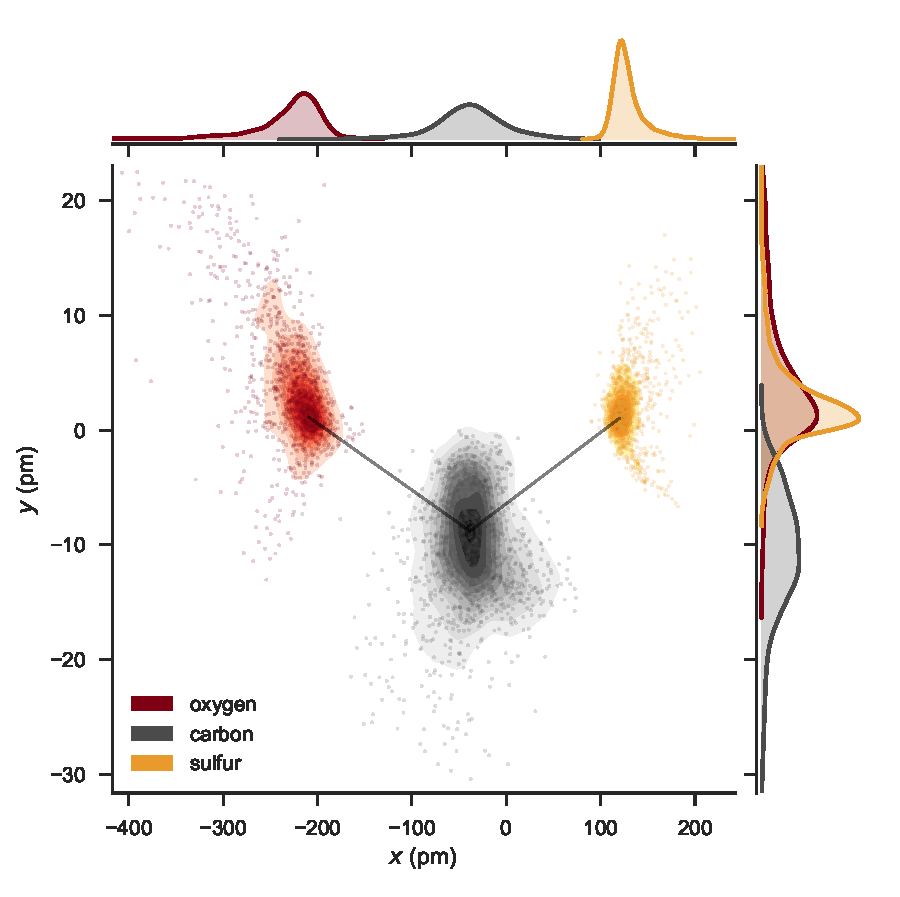
\includegraphics[width=\textwidth]{Plots/OCS2227fsMOGeometry}
  \caption[Scatter plot showing a reconstruction of the molecular geometry of \ch{OCS} following Coulomb explosion by a \SI{7}{\fs} laser pulse for the $(2,2,2)$ fragmentation channel.]
  {Scatter plot showing a reconstruction of the molecular geometry of \ch{OCS} following Coulomb explosion by a \SI{7}{\fs} laser pulse for the $(2,2,2)$ fragmentation channel. Each geometry is represented by three colored points, one for each atomic fragment; red for oxygen on the left, black for carbon in the center, and yellow for sulfur on the right. The colors were chosen to imitate the CPK coloring convention. Geometries are plotted such that the molecule's center of mass is at the origin to showcase the variance in each atomic fragment's position, and are rotated such that a vertical line bisects the \ch{O-C-S} bond angle. Bivariate kernel density estimates (KDE) with a Gaussian kernel, plotted as shaded-in contours, are used to estimate the the probability density of each atomic fragment's position (see section \ref{sec:kde} for a discussion of KDE's). Solid black lines are drawn between the peaks of each atomic fragment's kernel density estimate to illustrate the \emph{modal geometry} or most likely geometry. Along the top of the plot, univariate KDE's show the probability density of each atomic fragment's position along the $x$-axis, and the same is done for the $y$-axis along the right. The modal geometry is calculated to be $r_\mathrm{CO} = \SI{170}{\pico\m}$, $r_\mathrm{CS} = \SI{159}{\pm}$, $ \theta_\mathrm{OCS} = 173\degree$ while the average geometry of $r_\mathrm{CO} = \SI{193}{\pico\m}$, $r_\mathrm{CS} = \SI{168}{\pico\m}$, $ \theta_\mathrm{OCS} = 171\degree$ is slightly larger due to outliers. The molecule is almost straight but an aspect ratio of approximately $10:1$ is employed to showcase variability in the $y$-axis.}
  \label{fig:OCS2227fsMOGeometry}
\end{figure}

Before plotting, badly reconstructed geometries and duplicate geometries are filtered out. A badly reconstructed geometry satisfy at least one of three criteria. It (1) does not satisfy the KKT optimality conditions from section \ref{ssec:KKT} in which case the optimization algorithm is said to not have converged and \texttt{MultiStart} assigns such a geometry with an exit flag of $1$ making it easy to filter out such geometries. Or (2) it produces momentum vectors with a high absolute error when compared to the measured momentum vectors. We choose a threshold of $10^{-50}$ above which we say that the geometry is not precise enough to be a good reconstruction. The vast majority of reconstructions have significantly lower error ($10^{-59} - 10^{-54}$) and in general, geometries with a high absolute error do not satisfy (1) either. Or finally, (3) it lies very close to the box constraints (within $0.001$) that form our cuboid of physically realistic geometries in phase space. This usually indicates that the optimal geometry lies outside the constraints and that the solver asymptotically approached the boundary (due to the logarithmic barrier) in an attempt to converge on an optimal solution. Such bad geometries tend to also satisfy (1) and (2), but some redundancy is desirable to find all badly reconstructed geometries.

For our reconstruction, we configured \texttt{MultiStart} to use $50$ uniformly distributed starting points, which in hindsight was highly excessive. Out of $1,285$ sets of measured momentum vectors, we attempted to reconstruct each $50$ times, recovering $53,648$ geometries in total. $50,615$ represented duplicate geometries. Due to rounding errors involved with the comparison of floating-point numbers, we defined two triatomic geometries $i$ and $j$ to be duplicates if $\Delta_{ij} < 0.1$ where $\Delta_{ij} = |r_{12}^i - r_{12}^j| + |r_{23}^i - r_{23}^j| + |\theta^i - \theta^j|$ with bond lengths and angles being numerically described in picometers and degrees. After filtering out duplicate geometries, $3,033$ unique reconstructed geometries remain. $1,816$ had an exit flag of $1$ indicating a bad geometry (a non-optimal solution). No geometries with high error ($>10^{-50}$) were found, having all been previously found with an exit flag of 1. Then a further 91 geometries were found very close to the box constraints. Filtering out these $1,816 + 91 = 1,907$ bad geometries, we are left with $1,126$ ``good'' geometry reconstructions. $1,072$ were mapped to a single geometry, $18$ measurements to two distinct degenerate geometries, and $6$ to three distinct degenerate geometries. No measurement mapped to $4$ or more degenerate geometries, and $189$ measurements could not be reconstructed to satisfy our box constraints. In total, 2\% of measurements mapped to multiple degenerate geometries and $1,096$ measurements were successfully reconstructed, giving an 85\% success rate.

The recovered geometries are plotted in figure \ref{fig:OCS2227fsMOGeometry} and the geometries recovered for other laser pulse lengths (\SIlist{30;60;100}{\femto\s}) are plotted in appendix \ref{appx:supplementaryFigures} (figures \ref{fig:OCS22230fsMOGeometry}--\ref{fig:OCS222100fsMOGeometry}). The \SI{200}{\femto\s} data was not analyzed as the molecule seemed to have stretched too much for the lookup table reconstruction to seem trustworthy. Reconstruction statistics including success rate and number of degenerate geometries found for each pulse length is tabulated in table \ref{table:MOSuccess}. The modal and average geometries of for each pulse length are tabulated in table \ref{table:MOGeometries}.

% TODO: Discuss geometry plotting methods?

\begin{table}
  \myfloatalign
  \centering
  \begin{tabularx}{\textwidth}{cccc}
    \toprule
    Pulse length (\SI{}{\fs}) & Geometries & Reconstructions & Degenerate \\
    \midrule
    7 & 1285 & 1096 (85\%) & 18+6 (2.2\%) \\
    30 & 1501 & 1164 (76\%) & 62+30 (7.9\%) \\
    60 & 358 & 249 (70\%) & 15+6 (8.4\%) \\
    100 & 1056 & 694 (66\%) & 39+13 (7.5\%) \\
    \bottomrule
  \end{tabularx}
  \caption[Statistics for geometry reconstruction using constrained nonlinear optimization as a function of pulse length.]
  {Statistics for geometry reconstruction using constrained nonlinear optimization. The geometries column lists the number of experimental measurements (sets of momentum vectors) obtained, the reconstructions column lists the number and percentage of these measurements that were successfully reconstructed, and the degenerate column lists the number of measurements for which 2 and 3 degenerate geometries were found, respectively, and the percentage of successful reconstructions that yielded degenerate geometries. No measurement ever yielded more than 3 degenerate geometries.}
  \label{table:MOSuccess}
\end{table}

\begin{table}
  \myfloatalign
  \centering
  \begin{tabularx}{0.85\textwidth}{ccccccc}
    \toprule
    & \multicolumn{3}{c}{Modal geometry} & \multicolumn{3}{c}{Average geometry} \\
    Pulse length (fs) & $r_\mathrm{CO}$ & $r_\mathrm{CS}$ & $\theta_\mathrm{OCS}$ & $r_\mathrm{CO}$ & $r_\mathrm{CS}$ & $\theta_\mathrm{OCS}$ \\
    \midrule
    7 & 170 & 159 & 173 & 193 & 168 & 172 \\
    30 & 231 & 177 & 172 & 243 & 215 & 168 \\
    60 & 238 & 196 & 172 & 242 & 232 & 166 \\
    100 & 249 & 206 & 171 & 256 & 254 & 165 \\
    \bottomrule
  \end{tabularx}
  \caption[Average and modal geometries reconstructed using constrained nonlinear optimization as a function of pulse length.]
  {Average and modal geometries calculated from the geometries reconstructed using constrained nonlinear optimization as a function of pulse length. The bond lengths are given in picometers (\SI{e-12}{\m}) and the bond angles in degrees.}
  \label{table:MOGeometries}
\end{table}

% TODO: Discuss these tables.

\subsection{Comparision with the lookup table}
Comparing figures \ref{fig:OCS2227fsLTGeometry} and \ref{fig:OCS2227fsMOGeometry} we do not see much qualitative difference between the two. Figure \ref{fig:OCS2227fsMOGeometry} does have a greater number of reconstructions and data points. This is due to both the higher success rate (85\% versus 73\%) and since 500 more measurements were found since the lookup table was tested. Degenerate geometries contribute a small amount as well. The atomic positions exhibit greater variability in their positions, which may be because the optimization routine is able to reconstruct more extreme geometries than the lookup table could and with greater precision. The modal and average geometries calculated from both reconstructions are extremely similar.

While the overall geometry is not very different, the absolute errors on each geometry are much smaller. The lookup table produces geometries with absolute errors on the order of $10^{-48}$ at best due to its low resolution but the optimization routine finds geometries with errors on the order of $10^{-59} - 10^{-54}$, corresponding to an additional 3-5 decimal places of precision on the numerical values of the molecular parameters.

The optimization routine is also able to precisely find degenerate geometries by using multiple starting points, a task which would have been non-trivial for the lookup table.

\subsection{Investigating individual reconstructions} \label{ssec:weirdBonds}
Figure \ref{fig:OCS2227fsMOGeometry} provides an intuitive image of what a molecular geometry looks like, but it would be interesting to also see a distribution of bond lengths and bond angles to quantify the variability in each of these parameters. Correlations between the bond lengths and bond angles may also be looked at to study, for example, if longer \ch{C-O} bond lengths correspond to longer \ch{C-S} bond lengths, or if more bent geometries tend to have longer bond lengths. To visualize this relationship in figure \ref{fig:OCS2227fsMOGeometryPairs} we utilize a scatterplot matrix.

\begin{figure}
  \centering
  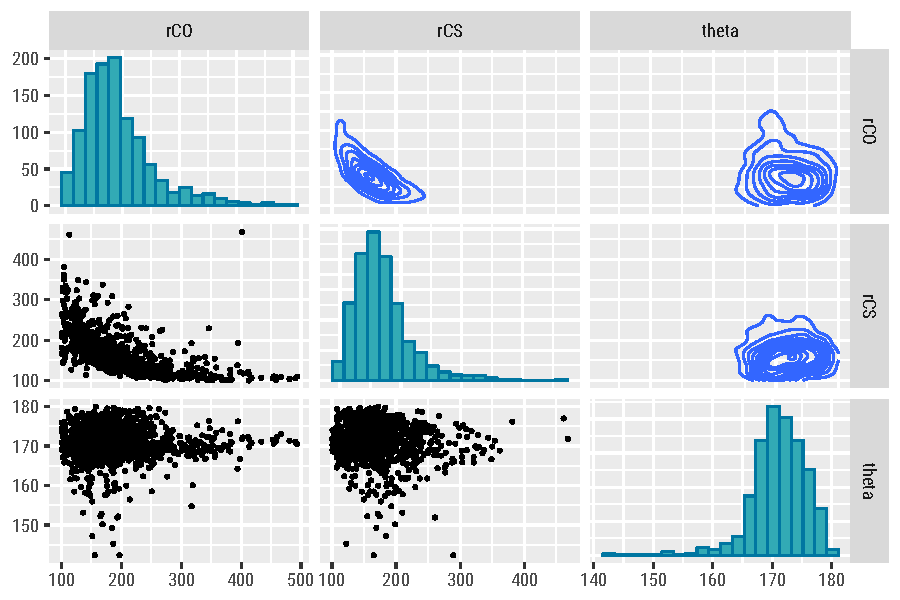
\includegraphics[width=\textwidth]{Plots/OCS2227fsMOGeometryPairs}
  \caption[Scatter plot matrix showing the bivariate relationship between the parameters $(r_\mathrm{CO}, r_\mathrm{CS}, \theta)$ for the reconstructions of the molecular geometry of \ch{OCS} following Coulomb explosion by a \SI{7}{\fs} laser pulse for the $(2,2,2)$ fragmentation channel.]
  {Scatter plot matrix showing the bivariate relationship between the parameters $(r_\mathrm{CO}, r_\mathrm{CS}, \theta)$ for the reconstructions of the molecular geometry of \ch{OCS} following Coulomb explosion by a \SI{7}{\fs} laser pulse for the $(2,2,2)$ fragmentation channel. On the diagonal, histograms show the distribution of bond lengths and bond angle for the reconstructed geometries (tick marks at the bottom of each column). Below the diagonal, scatter plots show the bivariate relationship between each molecular parameter. Above the diagonal, the same relationship is given using a contour plot instead.}
  \label{fig:OCS2227fsMOGeometryPairs}
\end{figure}

The bond length distributions on the diagonal of figure \ref{fig:OCS2227fsMomentum} are somewhat expected; they peak slightly above the equilibrium values indicating some molecular rearrangement and bond lengthening due to the molecule's interaction with the laser field. The bond angle distribution shows less variability suggesting that the molecule may have not had much time to bend yet, or that the laser's electric field primarily induces a lengthening in the bonds. This would seem expected as well, since the electric field's purpose is to quickly ionize the molecule which should cause the individual atoms to begin repelling each other as soon as the ionization occurs. % TODO: How similar is this to theoretical calculations?

What is very interesting, however, is the relationship between the two bond lengths, $r_\mathrm{CO}$ and $r_\mathrm{CS}$. We may intuitively expect both bond lengths to lengthen as the three atoms should repel each other in the $(2,2,2)$ charge state, or possibly to have one bond stretch while the other remains relatively constant. However, the reconstructions actually indicate the complete opposite---that while one bond stretches the other shrinks, almost following a reciprocal relationship. This effect becomes even more pronounced for reconstructions of molecular geometries exposed to longer pulse lengths (figures\ref{fig:OCS22230fsMOGeometryPairs} -- \ref{fig:OCS222100fsMOGeometryPairs}).

Such an unusual relationship suggests that our reconstruction efforts may have failed to account for a missing factor, or possibly that one of the assumptions we have made, particularly in simulating the Coulomb explosion (section \ref{sec:simulating}), is grossly invalid, or that some other part of our implementation requires revision. Unfortunately, to our knowledge no other studies performing geometry reconstruction using Coulomb explosion imaging have reported the correlations between their bond lengths and bond angles, so no comparisions or references can be made.\footnotemark~ When plotted, as in figure \ref{fig:OCS2227fsMOGeometry}, the geometries seem to be physically reasonable and so do the bond length and bond angle distributions on the diagonal of figure \ref{fig:OCS2227fsMOGeometryPairs}, it is only the correlations that do not. Analyzing the reconstructed geometries produced by the lookup table results in a very similar relationship between the bond lengths of reconstructed geometries.

\footnotetext{Private communication with collaborators suggests that other investigations have led to similar worrying results, leading to the abandonment of geometry reconstruction efforts.}

At this juncture, such worrying results force us to distrust the geometry reconstructions we have produced thus far. While the average geometries and overall dataset seems to be physically reasonable, the individual geometries seem to not make physical sense. Additionally, the same unusual relationship emerges out of at least two different reconstruction methods. For now we will move on to utilize the optimization routine to further investigate the nature of the degenerate geometries we are recovering, however we will come back and resolve this issue in the next chapter.

\section{Investigating degenerate geometries} \label{sec:optimizationDegeneracies}
The optimization approach should also be tested to study whether it can accurately reconstruct simulated geometries in the same manner we tested the Nelder-Mead simplex method (section \ref{ssec:simplexFail}) and the lookup table (section \ref{ssec:LTaccuracy}). We will also use this information to further investigate the nature of the degenerate geometries we are recovering.

The accuracy testing of the Nelder-Mead simplex method and the lookup table was relatively cursory, and could be made more thorough. We varied one molecular parameter at a time, which was however, sufficient to show the inadequecy of the simplex method. For a more thorough test, we will substantially vary all the molecular parameters by simulating the Coulomb explosion of geometries within a box in phase space described by $\SI{100}{\pico\meter} \le r_\mathrm{CO}, r_\mathrm{CS} \le \SI{500}{\pico\meter}$ and $\SI{140}{\degree} \le \theta \le \SI{180}{\degree}$. For a low-resolution test, we pick geometries $r_\mathrm{CO} \times r_\mathrm{CS} \times \theta_\mathrm{OCS}$ where $r_\mathrm{CO}$ and $r_\mathrm{CS}$ are sets containing $10$ uniformly spaced bond lengths between \SI{100}{\pico\meter} and \SI{500}{\pico\meter}, $\theta_\mathrm{OCS}$ is a set containing $10$ uniformly spaced bond angles between \SI{140}{\deg} and \SI{180}{\deg}, and $X \times Y = \lbrace (x,y) | x \in X \;\mathrm{and}\; y \in Y \rbrace$ denotes the cartesian product as expressed in set-builder notation \citep[p. 6]{Warner90}. Thus we are reconstructing $10^3 = 1,000$ geometries from simulated Coulomb explosions. We also perform a higher-resolution test using $20^3 = 8,000$ uniformly distributed geometries within the same box.

In both tests, we find that the optimization routine can reconstruct the simulated geometries in $98.5\%$ of cases using only a single starting guess. Each reconstruction takes approximately one second. In each of these reconstructions, the parameters of the recovered geometry numerically matched the original geometry up to several decimal places. The absolute error between the recovered and simulated momentum vectors was below $10^{-55}$ for $95\%$ of reconstructions, with the mean error being approximately $10^{-57}$, is 10 orders of magnitude lower than the absolute errors on momentum vectors retreived using the lookup table. Since we use the square of the $\ell_2$-norm to quantify the absolute error, this actually represents an improvement of approximately 5 orders of magnitude in accuracy over the lookup table. Using multiple starting points recovers geometries for the other $1.2\%$ of cases.

While the optimization routine recovered very precise geometries whose post-explosion momentum vectors very closely match the expected vectors, the geometries were not always the originally generated geometries which we expected. It seems that in about $5\%$ of cases, the routine returned a degenerate geometry. It is important to make the distinction that when the Nelder-Mead simplex method and the lookup table returned a different geometry than expected, it was a failure in recovering the exact geometry as the momentum vectors did not match closely resulting in a large absolute error (roughly $>10^{-46}$) (except for a small number of cases where it had found a degenerate geometry). However, in this case we are finding very precise reconstructions and each different geometry represents a degenerate geometry. To showcase the nature of these degenerate geometry, we plot arrows between the original (expected) geometry and the recovered degenerate geometry in figure \ref{fig:OCS222DegeneracyMaps}, which we will refer to as a \emph{degeneracy map}. If the recovered geometry was the original geometry as expected, then no arrow is plotted.

\begin{figure}
  \centering
  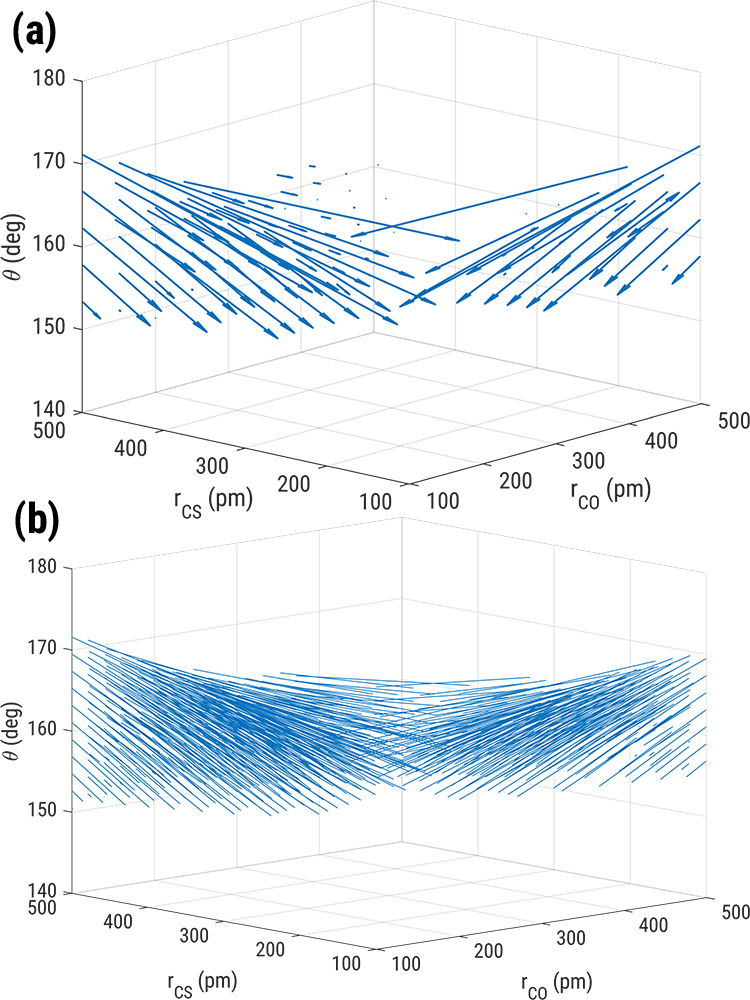
\includegraphics[width=\textwidth]{Plots/OCS222DegeneracyMap}
  \caption[Mapping between degenerate geometries for the \ch{OCS} $(2,2,2)$ molecule.]
  {Mapping between degenerate geometries for the \ch{OCS} $(2,2,2)$ molecule. The Coulomb explosion of (a) $1,000 \; (10^3)$ and (b) $8,000 \; (20^3)$ uniformly distributed geometries within a box in phase space described by $\SI{100}{\pico\meter} \le r_\mathrm{CO}, r_\mathrm{CS} \le \SI{500}{\pico\meter}$ and $\SI{140}{\degree} \le \theta \le \SI{180}{\degree}$ was simulated and then reconstructed using the momentum vectors of the atomic fragments that resulted from the simulations. If the reconstructed geometry matched the original geometry exactly, then no arrow is plotted. However, an (a) arrow or (b) line is plotted from the original expected geometry to the recovered geometry if it represented a degenerate geometry. Arrows and lines small enough that they resemble points indicate a slight numerical difference between the expected geometry and the reconstructed geometry, and do not neccessarily represent a degenerate geometry.}
  \label{fig:OCS222DegeneracyMaps}
\end{figure}

We see some patterns in the degenerate geometries recovered. Degenerate geometries exist only for molecules with bond angles between approximately \SI{150}{\deg} and \SI{170}{\deg} which includes a sizable minority of the molecules reconstructed as indicated by the bond angle distribution in figure \ref{fig:OCS2227fsMOGeometryPairs}. They also exist mainly for molecules exhibiting significant bond asymmetry and tend to be degenerate with another molecule that is more bent and has a smaller degree of bond length asymmetry. They also appear in two regions, one where the \ch{C-O} bond length is longer, and another where the \ch{C-S} bond length is longer. The discrete number of arrows figure \ref{fig:OCS222DegeneracyMapSD}(a) may suggest the existence of a discrete number of these degenerate geometries, however, repeating the test with a greater number of geometries produces very similar results except for a correspondingly higher density of lines, suggesting that regions exist in phase space where every geometry is degenerate with another, \ie~ that an uncountably infinite\footnotemark~ number of degenerate geometries exist.

\footnotetext{A countably finite set may refer to the set of integers $\mathbb{Z} = \lbrace 0, \pm 1, \pm 2, \dots \rbrace$, for example, which may be enumerated. An uncountably infinite set has the same cardinality as the set of real numbers $\mathbb{R}$ which cannot be enumerated \citep{Halmos17}.}

In these simulations we knew \textit{a priori} which geometry we expected to reconstruct, so we can assign a direction to each arrow. However, when reconstructing experimental data, we have no prior knowledge of what geometry we expected to recover, so the arrow could point in either direction. In some cases it might be possible to choose one degenerate geometry over the other(s) if one is physically unrealistic, \eg~ if it is very highly bent or exhibits an extreme bond length asymmetry.

\begin{figure}
  \centering
  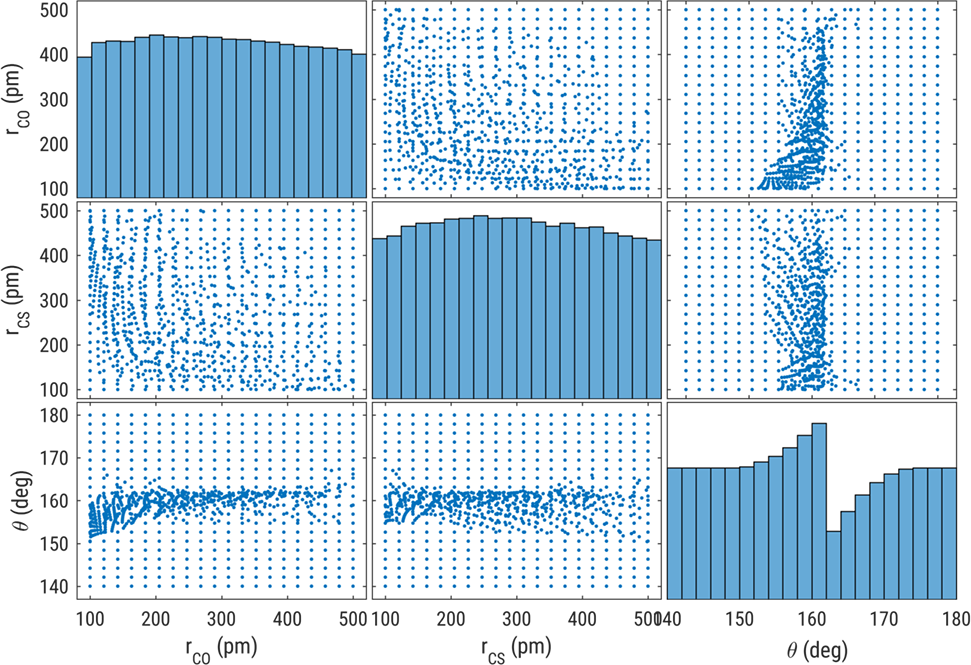
\includegraphics[width=\textwidth]{Plots/OCS222DegeneracyMapHDPairs}
  \caption[Scatter plot matrix showing the bivariate relationship between the parameters $(r_\mathrm{CO}, r_\mathrm{CS}, \theta)$ for the reconstructions of the molecular geometry of \ch{OCS} from momentum vectors obtained from simulated Coulomb explosions.]
  {Scatter plot matrix showing the bivariate relationship between the parameters $(r_\mathrm{CO}, r_\mathrm{CS}, \theta)$ for the reconstructions of the molecular geometry of \ch{OCS} from momentum vectors obtained from simulated Coulomb explosions of $8,000 \; (20^3)$ uniformly distributed geometries within a cuboid in phase space described by $\SI{100}{\pico\meter} \le r_\mathrm{CO}, r_\mathrm{CS} \le \SI{500}{\pico\meter}$ and $\SI{140}{\degree} \le \theta \le \SI{180}{\degree}$. On the diagonal, histograms show the distribution of bond lengths and bond angle for the reconstructed geometries with tick marks at the bottom of each column (no vertical scale is given for the histograms). Below the diagonal, scatter plots show the bivariate relationship between each molecular parameter. Above the diagonal, the same scatter plots are shown with the $x$ and $y$-axes interchanged to correspond with the axes labels and tickmarks.}
  \label{fig:OCS222DegeneracyMapHDPairs}
\end{figure}

To further visualize the set of geometries we recovered, we utilize a scatterplot matrix in figure \ref{fig:OCS222DegeneracyMapHDPairs} showing the bond length and angle distributions for the $8,000$ geometries used for accuracy testing as well as their bivariate relationships. It is interesting to note that whenever degenerate geometries exist, the more bent geometry is found. Perhaps these more bent solutions posess a larger \emph{basin of attraction}, which may or may not be strongly dependent on the optimization algorithm employed. It might be interesting to visualize them, possibly taking a similar approach as \citet{Asenjo13} who actually employ mathematical optimization methods to determine energy minimizing molecular structures. They observe basins with rather complicated boundaries, reminiscent of the beautiful and spatially chaotic patterns produced by the magnetic pendulum.

For the feasibility of geometry reconstruction, however, this result raises additional issues past the unusual bond length correlations found in the previous section. Even when the measured momentum vectors can be mapped to a molecular geometry very precisely, the existance of multiple solutions corresponding to very different geometries may make it impossible to perform accurate geometry reconstructions, especially when multiple degenerate geometries represent physically realizable geometries. Table \ref{table:lookupTableSuccess} also suggests the existence of triply degenerate geometries, which may further complicate the task of geometry reconstruction.

Interestingly, we find that we recover degenerate geometries approximately $5\%$ of the time while \citet[supplementary information]{Kunitski15} report finding degenerate geometries approximately $10\%$ of the time, although they chose to disregard them for their analyses.

We considered whether these degeneracies could arise due to our choice of momentum convention in section \ref{sec:conventions} however our convention simply rotates the three momentum vectors such that the carbon's momentum vector lies along the $+x$-axis and all three momentum vectors lie in a plane. The length of the momentum vectors and the relative angles between them remain unchanged, and so two different geometries producing different momentum vectors cannot result in the same set of vectors after rotation into our convention, unless they represent degenerate geometries.

\section{Conclusions}
\emph{Geometries may be reconstructed quickly and precisely using constrained nonlinear optimization}---This approach represents a significant improvement over the geometry reconstructions provided by the lookup table. Reconstructing a single geometry can be done in approximately one second, which is faster than the lookup table if enhanced precision is desired. Furthermore, the recovered molecular parameters are orders of magnitude more precise than those provided by the lookup table, and degenerate geometries may be found precisely.

%\subsection{Lessons learnt}
%\emph{Individual reconstructed geometries must be investigated}--- \\
%
%\noindent
%\emph{Regions in phase space containing degenerate geometries make geometry reconstruction more difficult}--- 
%
%\subsection{Future directions}
%\emph{Reconstruction of larger molecules}--- \\
%
%\noindent
%\emph{More efficient optimization}---
\chapter{Uncertainty quantification in geometry reconstruction} \label{ch:uncertainty}

\vspace{-1.5 em}
\begin{addmargin}[-0.5cm]{0cm}
  \minitoc
\end{addmargin}
\hrule
\vspace{1.5 em}

In the previous two chapters, we approached the task of geometry reconstruction using two approaches, a lookup table which was only feasible for the reconstruction of triatomic molecules, and the more sophisticated optimization approach. We also ended on a rather troubling note regarding the feasibility of geometry reconstruct, namely that the reconstructed geometries exhibited unusual bond length correlations (section \ref{ssec:weirdBonds}) and that degenerate geometries can be found in large region of phase space (section \ref{sec:optimizationDegeneracies}).

In this chapter we will begin by tackling the important task of quantifying the uncertainty on our geometry reconstructions, which surprisingly has not been performed by any previous study. We will take a heuristic approach, which provides some valuble estimates on the amount of uncertainty to expect and will help resolve the issue of unusual bond length correlations. A more rigorous and sophisticated approach of uncertainty quantification in the Bayesian inference framework was attempted and although it has stagnated, the motivation and methodology of this approach will be discussed.

\section{Uncertainty on a reconstructed geometry} \label{sec:heuristicApproach}
The question of interest in this section is, \textit{``how does uncertainty in the measured momentum vectors affect the uncertainty of the reconstructed geometry?''} We have already calculated the uncertainty on the momentum vectors in section \ref{ssec:measurementUncertainty} but we cannot derive an analytic formula for the uncertainty on the molecular parameters or the atomic positions.

\subsection{A heuristic approach}
We will take a very basic approach here by attempting to generalize a simple result for the propagation of error through a monotonically increasing function. A monotonically increasing function is always increasing, that is, it always has a positive first derivative.

If a particular measurement $\bar{x}$ of a variable $x$ carries some uncertainty $\epsilon$ such that the true value of $\bar{x}$ lies within some interval $\bar{x} - \epsilon \le \bar{x} \le \bar{x} + \epsilon$ then the true value of some arbitrary monotonically increasing scalar function $f(x)$ that is dependent on the value of the measurement will lie within some interval
\begin{equation}
  f(\bar{x} - \epsilon) \le f(\bar{x}) \le f(\bar{x} + \epsilon)
\end{equation}

Now if we relax the condition that $f$ be a monotonically increasing function, then the true value of $f(\bar{x})$ can take on any value that $f$ attains within the interval $\bar{x} - \epsilon \le \bar{x} \le \bar{x} + \epsilon$, and we can say very generally that it lies between
\begin{equation} \label{eq:shittyInterval}
  \min_{\displaystyle \bar{x} - \epsilon \le x \le \bar{x} + \epsilon} \; f(x)
  \le f(\bar{x})
  \le \max_{\displaystyle \bar{x} - \epsilon \le x \le \bar{x} + \epsilon} \; f(x)
\end{equation}
which however, may not yield a useful interval, especially in the presence of discontinuities or divergences. However, for finite-valued and well-behaved functions that do not change rapidly within the interval $\bar{x} - \epsilon \le \bar{x} \le \bar{x} + \epsilon$, \eqref{eq:shittyInterval} may provide a useful upper bound on the uncertainty in $f(\bar{x})$. This could be particularly accurate for small neighbourhoods about $\bar{x}$. As geometry reconstruction produces physically reasonable values for the molecular parameters without any discontinuties or divergences, we will attempt to use this idea to quantify the uncertainty on a geometry's reconstruction.

Before generalizing these two ideas for multivariable measurements and functions, it will be helpful to look at this idea for the case of measurement of a vector of two variables $\bar{\mathbf{x}} = (\bar{x}_1, \bar{x}_2)$ with an uncertainty described by the vector $\bm{\epsilon} = (\epsilon_1, \epsilon_2)$ and error propagation through a vector-valued function of two variables $\mathbf{f}(\mathbf{x}) = (f_1(\mathbf{x}), f_2(\mathbf{x}))$. We will treat $\mathbf{f}(\mathbf{x})$ as non-parametric and assume that it has no analytic form, \ie~ as a \emph{black box} function as the mapping from momentum vector measurements to geometries cannot be parameterized or given in any analytical form.

In this case the true value of $\bar{\mathbf{x}}$ lies within a box described by $\bar{x}_1 - \epsilon_1 \le \bar{x}_1 \le \bar{x}_1 + \epsilon_1$ and $\bar{x}_2 - \epsilon_2 \le \bar{x}_2 \le \bar{x}_2 + \epsilon_2$ in the $x_1x_2$ plane. If both $f_1(\mathbf{x})$ and $f_2(\mathbf{x})$ depend monotonically on $x_1$ and $x_2$ then determining the range of possible values of $\mathbf{f}(\bar{x})$ would be simple. Evaluating $\mathbf{f}(\mathbf{x})$ for 
\begin{equation} \label{eq:endpoints}
\mathbf{x} \in \mathbf{x}_\mathrm{ep}
  % = \lbrace (\bar{x}_1 \pm \epsilon_1, \bar{x}_2 \pm \epsilon_2) \rbrace
  = \left\lbrace
    \begin{pmatrix} x_1 - \epsilon_1 \\ x_2 - \epsilon_2 \end{pmatrix},
    \begin{pmatrix} x_1 - \epsilon_1 \\ x_2 + \epsilon_2 \end{pmatrix},
    \begin{pmatrix} x_1 + \epsilon_1 \\ x_2 - \epsilon_2 \end{pmatrix},
    \begin{pmatrix} x_1 + \epsilon_1 \\ x_2 + \epsilon_2 \end{pmatrix}
  \right\rbrace
\end{equation}
where $\mathrm{ep}$ is an abbreviation for ``endpoints'' (as $\mathbf{x}_\mathrm{ep}$ denotes the set of endpoints for the box containing feasible values of $\mathbf{x}$ in the $x_1x_2$ plane) would produce $4$ point in the $f_1f_2$ plane, whose set we denote by $\mathbf{f}_\mathrm{ep}$ and whose rectangular boundary encloses the possible values of $f(\bar{x})$. Thus the propagation of uncertainty in this case can be thought of a mapping from a rectangle in the $x_1x_2$ plane to a rectangle in the $f_1f_2$ plane.

If $f_1$ and $f_2$ do not depend monotonically on $x_1$ and $x_2$, then values of $x_1$, $x_2$ between the endpoints may produce values of $f_1$,$f_2$ that lie outside the rectangular boundary. A further heuristic would be to not only look at the endpoints, but also a set of uniformally distributed points in the $x_1x_2$ plane within the box of possible values for $\mathbf{x}$. In this case, the propagation of uncertainty can be thought of as a mapping from a rectangle in the $x_1x_2$ plane to an arbitrary region in the $f_1f_2$ plane whose boundary may not be rectangular anymore, or even a single region. In the case of a more complicated boundary, we will generalize \eqref{eq:shittyInterval} by describing the boundary using a \emph{convex hull}. The convex hull $C$ of a set of points $S = \lbrace p_1, p_2, \dots, p_n \rbrace$ where $p_i \in \mathbb{R}^m$ for all $i$ can be expressd mathematically as
\begin{equation}
C = \left\lbrace\left.
  \sum_{i=1}^n \lambda_i p_i \right|
  \lambda_i \ge 0
  \;\; \mathrm{and} \;\;
  \sum_{i=1}^n \lambda_i = 1
  \right\rbrace
\end{equation}
An analogy in two dimensions would be to stretch a rubber band around the set of points and let it rest, its final shape being the convex hull.

%by the set of convex combinations of the points in $\mathbf{f}_\mathrm{ep}$,
%\begin{equation}
%  \displaystyle
%  \left\lbrace\left.
%  \sum_{\mathbf{f} \in \mathbf{f_i}_\mathrm{ep}}^{|\mathbf{f}_\mathrm{ep}|}
%  \alpha_i\mathbf{f_i}
%  \right| \alpha_i \ge 0 \; \mathrm{and} \;
%  \sum_i^{|\mathbf{f}_\mathrm{ep}|} \alpha_i = 1
%  \right\rbrace
%\end{equation}
%which is the convex hull of the set of points contained in $\mathbf{f}_\mathrm{ep}$, discussed further in the next subsection.

Extending this idea to our problem of geometry reconstruction, we have $9$ measurements $\bar{\mathbf{p}} = (\bar{p}_1, \dots, \bar{p}_9)$ with uncertainty $\bm{\epsilon} = (\epsilon_1, \dots, \epsilon_9)$ and we are interested in the range of possible geometries as produced by $\mathbf{g}(\mathbf{p}) = (r_{12}(\mathbf{p}), r_{23}(\mathbf{p}), \theta(\mathbf{p}))$. The possible values of the momentum components are contained within a $9$-dimensional hyperrectangle or box in momentum space, and we would like to obtain a $3$-dimensional region in phase space describing the set of possible geometries that the measurement could correspond to. Generating a set of $N$ uniformally distributed points within the $9$-dimensional box would produce $N^9$ sets of momentum vectors, each of which must be reconstructed. This represents a rather unfeasible number of reconstructions to perform, thus we will start by looking at the set of endpoints only, which contains $512$ ($2^9$) sets of momentum vectors. Attempting to reconstruct a geometry for each set of momentum vectors will ideally provide us with $512$ geometries that together give us some idea into the range of possible geometries the measurement could possibly belong to. By only reconstructing the endpoints of our box in momentum space, we may be underestimating the range of possible geometries as points within the box may produce more extreme geometries when reconstructed.

% % r_CO=131.677 pm, r_CS=187.161 pm, theta=169.42 deg
To carry out this idea for geometry reconstruction, we randomly chose a representative geometry, $(r_\mathrm{CO}, r_\mathrm{CS}, \theta) = (\SI{130}{\pico\m}, \SI{190}{\pico\m}, \SI{169}{\degree})$ that does not lie in any of the degenerate regions discussed in figure \ref{fig:OCS222DegeneracyMaps} to avoid having to account for degenerate geometries. Simulating a Coulomb explosion using this geometry as the intial condition yields a set of momentum vectors, upon which we artifically placed an uncertainty of $5\%$ for each momentum component such that $\bm{\epsilon} = 0.05\mathbf{p}$, producing $512$ sets of momentum vectors corresponding to the corners of the $9$-dimensional box in momentum space, that is, a 9-dimensional version of \eqref{eq:endpoints}. Reconstructing a geometry for each set of momentum vectors, we obtain $512$ geometries and all $512$ sets of momentum vectors were successfully mapped to a unique geometry. Histograms showcasing the bond length and bond angle distributions of these reconstructed geometries are plotted in figure \ref{fig:OCS222Uncertainty} along with scatter plots showcasing the bivariate relationships between the three molecular parameters.

\begin{figure}
  \centering
  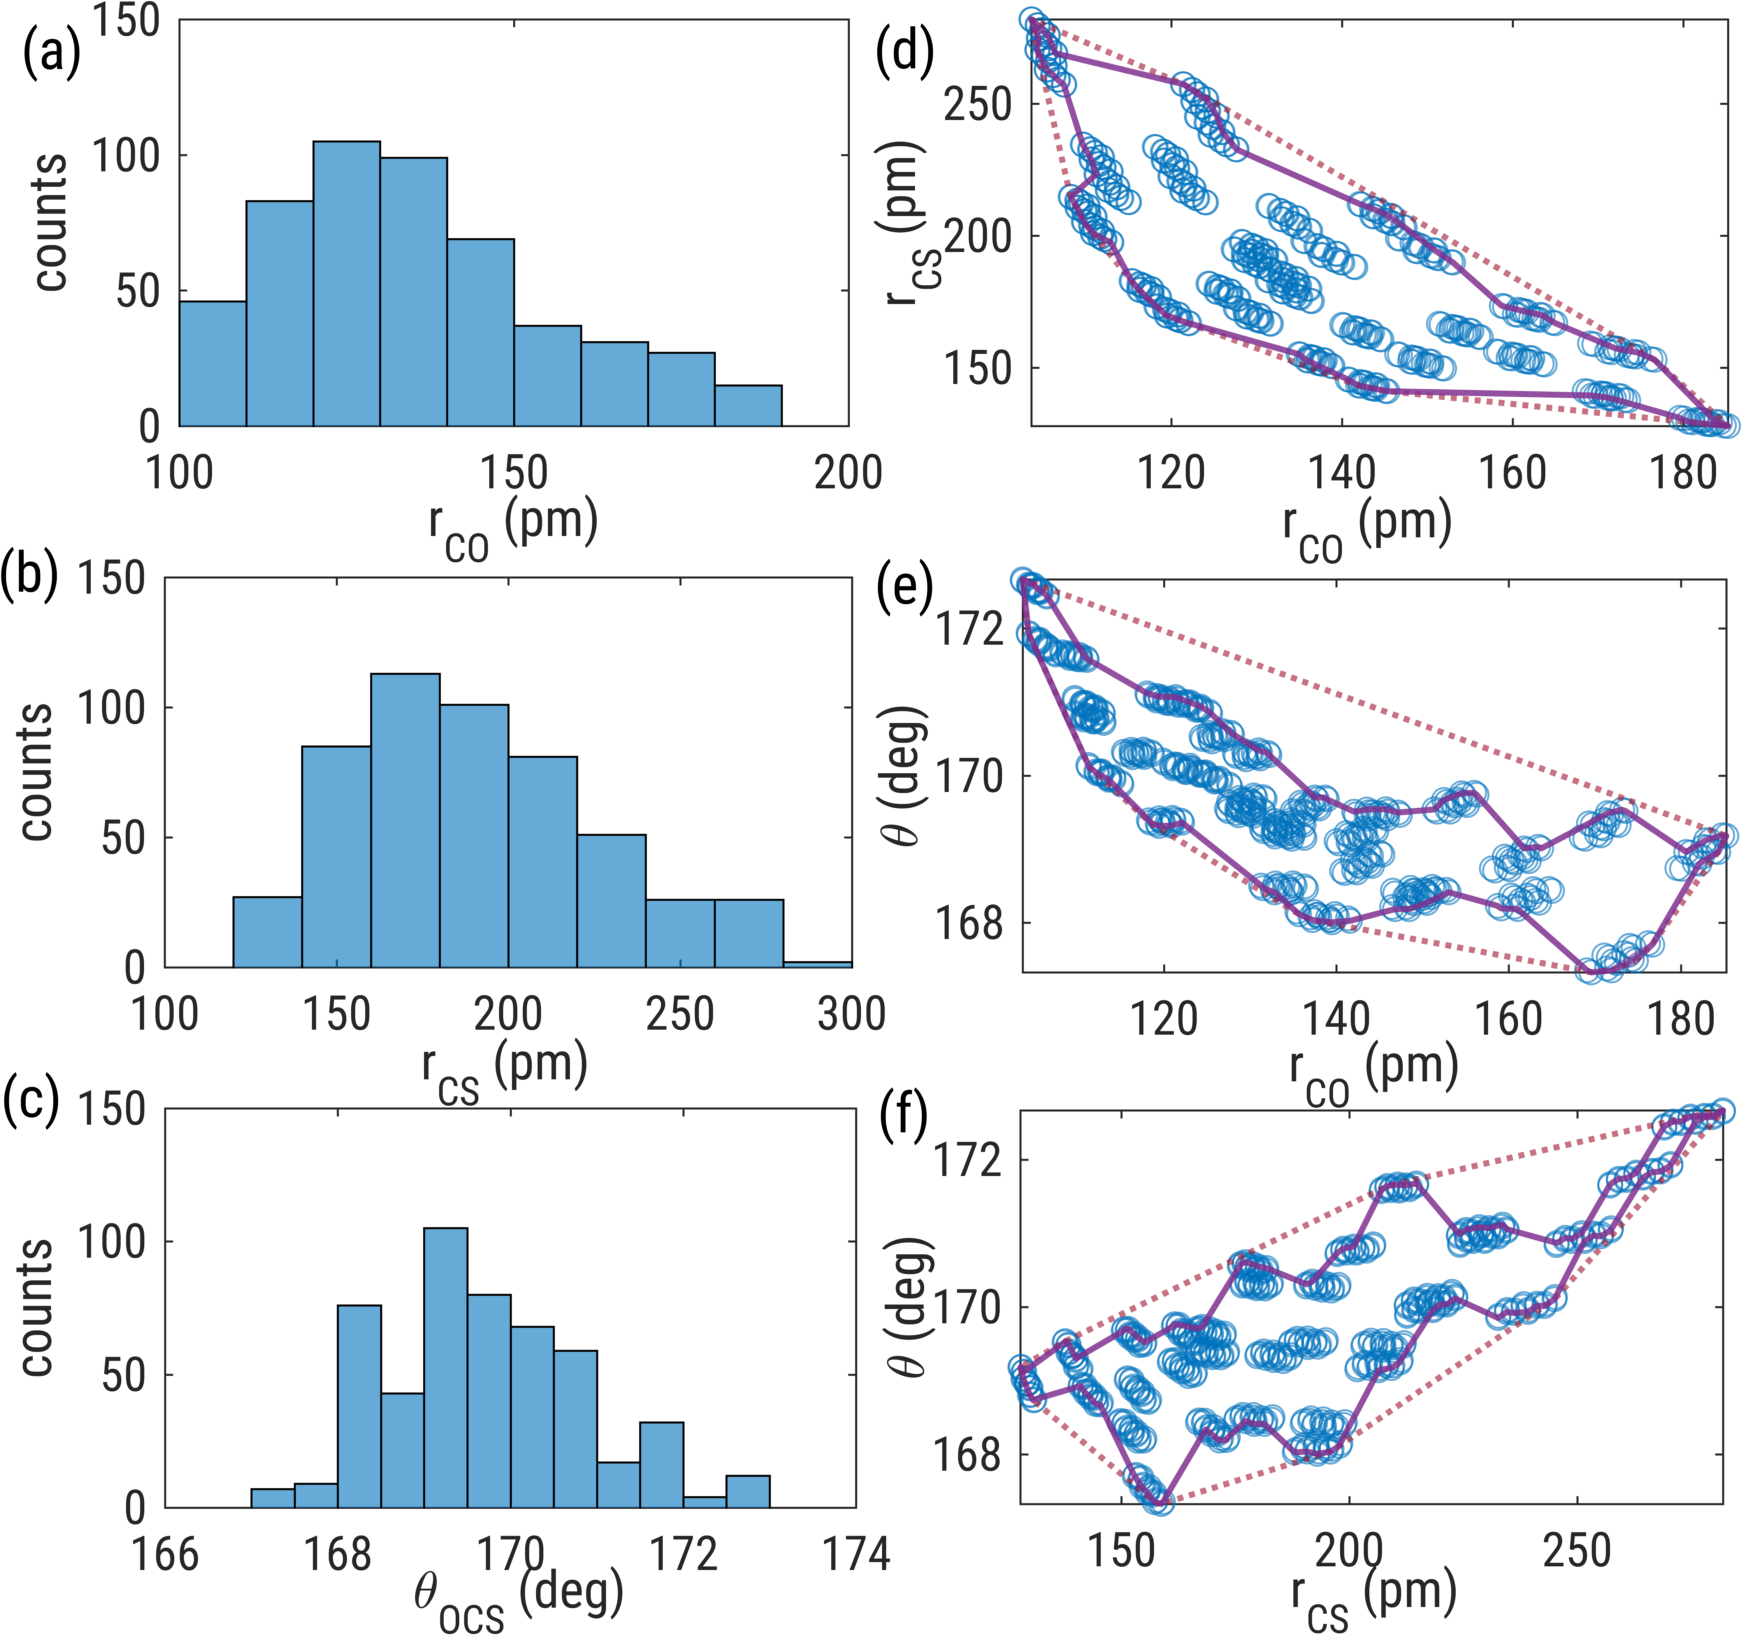
\includegraphics[width=\textwidth]{Plots/OCS222Exploration1_5percent}
  \caption[A heuristic estimate on the range of possible \ch{OCS} $(2,2,2)$ geometries that may be reconstructed assuming a true geometry of $(r_\mathrm{CO}, r_\mathrm{CS}, \theta) = (\SI{130}{\pico\m}, \SI{190}{\pico\m}, \SI{169}{\degree})$ and $5\%$ uncertainty on the measured momentum vectors.]
  {A heuristic estimate on the range of possible \ch{OCS} $(2,2,2)$ geometries that may be reconstructed assuming a true geometry of $(r_\mathrm{CO}, r_\mathrm{CS}, \theta) = (\SI{130}{\pico\m}, \SI{190}{\pico\m}, \SI{169}{\degree})$ and $5\%$ uncertainty on the measured momentum vectors. Histograms showcase the (a) \ch{C-O} bond length, (b) \ch{C-S} bond length, and (c) bond angle distributions of the reconstructed geometries. Scatter plots showcase the bivariate relationships between (d) $r_\mathrm{CO}$ and $r_\mathrm{CS}$, (e) between $r_\mathrm{CO}$ and $\theta$, and (f) between $r_\mathrm{CS}$ and $\theta$. Each reconstructed geometry is plotted as an open blue circle. The boundary of the set of reconstructed geometries is calculated using two methods and plotted; The dotted red line denotes the convex hull and the solid purple line denotes the alpha shape (using (d) $\alpha=15$, (e) $\alpha=22$, and (f) $\alpha=30$) of the set of points.}
  \label{fig:OCS222Uncertainty}
\end{figure}

We immediately see that a strikingly wide range of geometries are reconstructed assuming the momentum components carry an uncertainty of only $5\%$. Inspection suggests that the bond length and bond angle distributions roughly form a Gaussian distribution about the true parameters. The distributions encompass a wide range of possible bond lengths, \SI{80}{\pico\m} for the \ch{C-O} bond and \SI{175}{\pico\m} for the \ch{C-S} bond. The variability in the bond angle is not as extreme, encompassing a \SI{6}{\degree} range of possible bond angles.

The bivariate relationships shown in figures \ref{fig:OCS222Uncertainty}(d)-(f) suggest the range of possible geometries. Interestingly, the bond length correlation in figure \ref{fig:OCS222Uncertainty}(d) seems to follow a reciprocal relationship, a strikingly similar one to the unusual one observed in the reconstructions of experimental data. This suggests that uncertainty in the momentum measurments may lead to the reconstruction of a geometry with asymetrically stretched bonds, and that the unusual relationship we observed in section \ref{ssec:weirdBonds} may have been a manifestation of measurement uncertainty and due to the highly sensitive nature of geometry reconstruction.

Placing a larger uncertainty on the momentum vector components further stretches the shape of the set of points in figure \ref{fig:OCS222Uncertainty}(d), modifying it to further resemble the more extreme reciprocal relationship between $r_\mathrm{CO}$ and $r_\mathrm{CS}$ found for longer pulse lengths (see figures \ref{fig:OCS22230fsMOGeometryPairs} -- \ref{fig:OCS222100fsLTGeometryPairs}). 

Exposing the molecule to longer laser pulses provides a longer amount of time for the molecule to rearrange and may impart the atomic fragments with a larger initial momentum, thus decreasing the certainty with which the measured momentum vectors correspond to the true geometry. If we take a reciprocal relationship to be a signature indicating that too much measurement uncertainty is present for trustworthy geometry reconstructions, then we must conclude that even an uncertainty as low as a few parts per hundred in the momentum vector components is ``too much'' and that geometry reconstruction using Coulomb explosion imaging is unfeasible under such conditions.

We may use the area formed by the set of points in figures \ref{fig:OCS222Uncertainty}(d)-(f), plotted as red dotted lines by the use of a convex hull, as a quantitative measure of uncertainty. Another boundary may be provided by the \emph{alpha shape} of the set of points, plotted as solid purple lines.

An interesting observation resulting from the close inspection of the open blue circles in figures \ref{fig:OCS222Uncertainty}(d)-(f) is the clustering of geometries in phase space as geometries seem to cluster in little groups. Each geometry is actually paired with one other geometry (close inspection of the open blue circles should reveal that they appear in pairs, sometimes appearing as a single blurred circle) so that $256$ points are visible unless the scatter plots are very closely inspected. As we picked one of two extreme values, $\bar{p} - \epsilon$ and $\bar{p} + \epsilon$ for each momentum component, each component may be responsible for the ``splitting of the geometries'' into pairs or clusters. This suggests that some uncertainty in certain momentum components may have a greater effect on the uncertainty of reconstructed geometries.

\subsection{Convex hulls and alpha shapes}
To quantify the uncertainty in the geometries, we will use two useful concepts from computational geometry, namely convex hulls and alpha shapes, which allow us to assign a shape and a volume to a set of points, and thus provide an additional hueristic quantitative measure of uncertainty.

The convex hull of a set of points $S$ is the set of all convex combinations of its points. An analogy would be to stretch a rubber band around the set of points and let it rest, its final shape being the convex hull.

Many algorithms exist to calculate the convex hull of a set of points, especially in 2 or 3 dimensions.

The concept of an alpha shape is a generalization of the convex hull first introduced by \citet{Edelsbrunner83} for two-dimensional shapes, then for three-dimensional shapes \citep{Edelsbrunner94}. Interestingly, alpha shapes have been used to analytically compute shapes for macromolecules such proteins and estimate their molecular areas and volume \citep{Liang98}. An interesting analogy of alpha shapes uses ice cream scoopers.

The nice thing about convex hulls is that they are unique for each set of points, while multiple distinct alpha shapes exist. This is a desirable property of alpha shapes as there is no formal concept of shape so no algorithm can determine the correct shape for a set of points. However, the concept allows for an $\alpha$ to be picked that produces the most desirable shape. 

While a very haphazard measure of uncertainty, they are much easier to employ than the sophisticated uncertainty quantification framework of Bayesian inference (section \ref{sec:uncertaintyBayesian}) and will come in handy when we perform some exploratory uncertainty analysis in section \ref{sec:uncertaintyAnalysis}. Our needs are rather basic at this point.

We end by providing a cool figure showcasing the three-dimensional convex hull and alpha shape in molecular phase space.

% figure Z here

\section{Determining the sources of uncertainty} \label{sec:sourceUncertainty}
We saw in figures \ref{fig:OCS222Uncertainty} that certain momentum components may have a greater effect on the uncertainty on a reconstructed geometry, or that geometry reconstruction is more sensitive to changes in certain momentum components over others.

We will attempt to explore this effect and pinpoint the momentum components responsible for introducing the most (and the least) uncertainty in the reconstructed geometries. To do this for the oxygen's $p_x$ component for example, we will look at the $256$ geometries reconstructed using the $256$ sets of momentum vectors where $5\%$ was added to the oxygen's $p_x$ component, and plot their position in phase space in the $r_\mathrm{CO}-r_\mathrm{CS}$ plane. Doing this for each component, we produce $9$ plots in total, one for each momentum component, as shown in figure \ref{fig:OCS222DeterminingSource}.

\begin{figure}
  \centering
  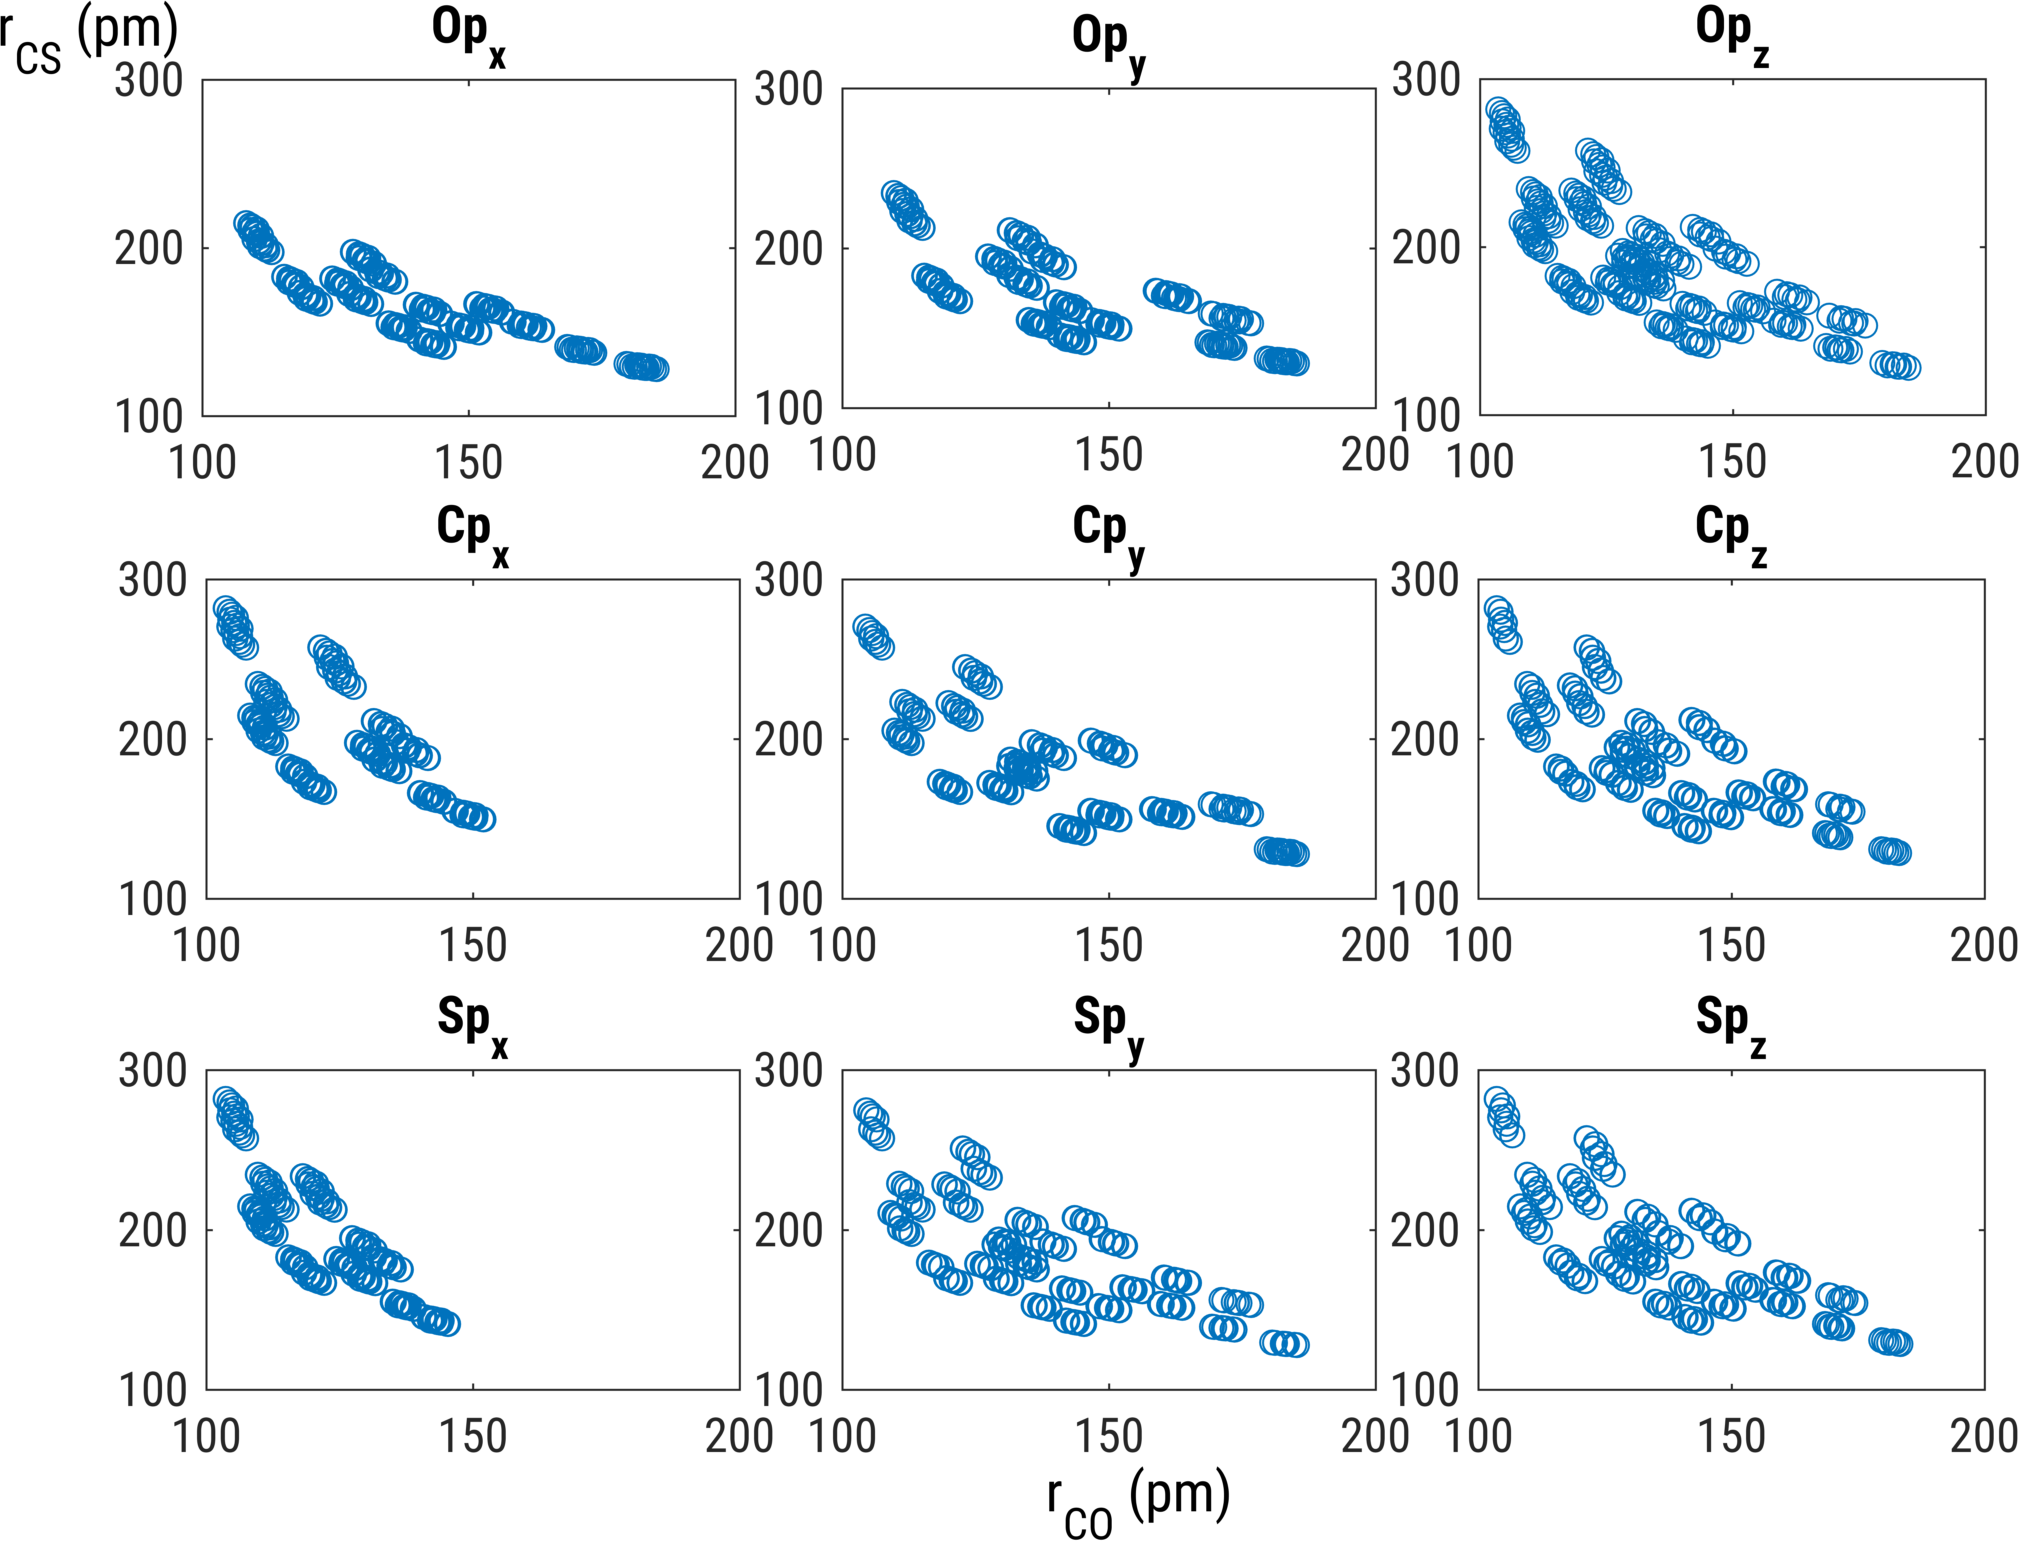
\includegraphics[width=\textwidth]{Plots/OCS222Exploration2}
  \caption[Scatter plots providing a heuristic estimate on the range of possible \ch{OCS} $(2,2,2)$ geometries that may be reconstructed assuming a true geometry of $(r_\mathrm{CO}, r_\mathrm{CS}, \theta) = (\SI{130}{\pico\m}, \SI{190}{\pico\m}, \SI{169}{\degree})$ and $5\%$ uncertainty on the measured momentum vector components except for the single component indicated in the title of each scatter plot.]
  {Scatter plots providing a heuristic estimate on the range of possible \ch{OCS} $(2,2,2)$ geometries that may be reconstructed assuming a true geometry of $(r_\mathrm{CO}, r_\mathrm{CS}, \theta) = (\SI{130}{\pico\m}, \SI{190}{\pico\m}, \SI{169}{\degree})$ and $5\%$ uncertainty on the measured momentum vector components except for the single component indicated in the title of each scatter plot. For each plot the \ch{C-O} bond length is plotted on the horizontal axis and the \ch{C-S} bond length on the vertical axis.}
  \label{fig:OCS222DeterminingSource}
\end{figure}

We immediately see that some momentum components are responsible for larger variations in the reconstructed geometries than others. The carbon and sulfur's $p_x$ components seem responsible for almost doubling the variability in the \ch{C-O} bond length while the oxygen's $p_x$ component seems responsible for almost doubling the variability in the \ch{C-S} bond length. Very close inspection reveals that removing the uncertainty on the oxygen's $p_z$ component removes the pairing up of the geometries, suggesting that uncertainty on oxygen's $p_z$ component is largely irrelevant for geometry reconstruction.

The exact dependence observed in figure \ref{fig:OCS222Uncertainty}, that is, which components contribute more to the uncertainty of reconstructed geometries, may be due to experimental setup factors such as the polarization of the laser's electric field or the initial orientation of the molecule at the start of the Coulomb explosion. It may also depend on the convention used to rotate and describe the momentum vectors (section \ref{sec:conventions}).

Further investigation is certainly warranted, especially if one aims to design a Coulomb explosion imaging experiment for the purposes of minimizing errors in geometry reconstruction. Molecules may be oriented to minimize errors in geometry reconstruction, for example.

\section{Exploratory uncertainty analysis} \label{sec:uncertaintyAnalysis}
Our main intentions in this chapter are twofold. Firstly, to suggest that measurement uncertainty is responsible for the asymmetric bond length correlations that arise out of both reconstruction methods, and secondly, to suggest that uncertainty on certain momentum components results in a larger error on the reconstructed geometries which, upon further investigation, may be exploited in the design of CEI experiments for minimizing errors in geometry reconstruction.

In this section we will simply describe some further investigations or rather, \emph{explorations}, that may be carried out to study the effects of measurement uncertainty on the geometry reconstruction process.

A major drawback to the analysis performed in section \ref{sec:heuristicApproach} is the large number of geometries that must be reconstructed, $2^9$ for a triatomic molecule if only the endpoints of the box in momentum space are used. For a molecule with $N$ atoms, this scales exponentially as $2^{3N}$. To reduce the number of reconstructions that must be performed, a simplified version of the analysis in section \ref{sec:sourceUncertainty} may be performed first. By adding uncertainty on each component one-by-one, $2\times3N$ different sets of momentum vectors are produced which may quickly reconstructed, hinting at which momentum components produce large errors in the reconstructed geometries, and which do not. The components that do not introduce large errors may be ignored when constructing the $3N$-dimensional box in momentum space, reducing the number of geometries to be reconstructed by a factor of $2$ for each component that introduces very small errors.

In using a convex hull or alpha shape to describe the set of possible geometries, we are neglecting that certain regions of phase space may contain a higher density of geometries than others. Thus, while the region may be quite large by itself, the vast majority of reconstructed geometries may lie within a smaller region of phase space. To determine the density of reconstructed geometries in phase space, momentum values lying between the end points must be reconstructed as well. This may be quite time-consuming to perfom and may require the reconstruction of many more than $2^{3N}$ geometries but may shed further insight. It will also be different for each measurement and thus, cannot be done for a data set consisting of hundreds of momentum vectors. A three-dimensional kernel density estimate may then provide an approximation to the probability distribution for the true geometry.

% Let's put a range of uncertainties on the momentum vectors and observe how much uncertainty we have on the reconstructed geometries. We will use the widths of the distributions and the convex hull and alpha shape areas and volumes to quantify the uncertainty with the aim of finding how uncertainty in geometry reconstruction varies as a function of uncertainty in the momentum vectors.

\section{Uncertainty quantification using Bayesian inference} \label{sec:uncertaintyBayesian}
The heuristic uncertainty quantification performed in the first two sections has provided significant insights on the process of geometry reconstruction, and emphasized the large effect that measurement uncertainty must have played in our reconstruction of experimental data. This further highlights the importance of tackling the task of uncertainty quantification in a rigorous and sophisticated manner, in which case the Bayesian inference framework provides a .

% Philosophy? objective vs. subjective Bayes, frequentist vs. Bayesian, etc.
The Bayesian point of view provides a more natural and intuitive way of thinking about uncertainty in the physical sciences.

% Why Bayesian inference is perfect for inverse problems.

Bayesian statistics actually predates the much more commonly taught frequentist statistical methods but has made a strong resurgence in recent years due to rising computational abilities and more recently, available software for parameter estimation in statistical models using Markov chain Monte Carlo.

A well-known article authored by \citet{Efron86} and titled ``Why isn't everyone a Bayesian?'' argues in favor of the more intuitive and powerful Bayesian framework . \citet{Cousins95} authored a similarly titled article, ``Why isn't every physicist a Bayesian?'' comparing both the classical and Bayesian frameworks in the context of particle physics. A more recent article on the subject authored by \citet{Lyons12} appeared in \emph{Physics Today}. Extensive review articles have been written on the more general subject of Bayesian inference in physics and include numerous examples and case studies \citet{vonToussaint11,Dose03,Dagostini03}. Although not particularly writing about Bayesian inference, \citet{Hogg10} provide a rather excellent and extensive tutorial in fitting data to models in the form of an article, and include numerous excercises relying on the use of Bayesian inference.

Numerous textbooks exist on the topic. \citet{Gelman14} provide an excellent introduction to Bayesian data analysis, especially the theory while \citet{Kruschke14} provide a very solid and easy to follow introduction especially to Markov chain Monte Carlo methods which we cover in more depth later.

\subsection{Elementary concepts}
% Ideas?: credibility, models, parameters, distributions.
% Theory?: Bayes Theorem, prior predictive, posterior, posterior mode (read up).
% Bayes’ theorem: we just need to do a multi-dimensional integral

\subsection{Markov chain Monte Carlo}
% The basic idea
Performing the multi-dimensional integral can be very difficult. The integral is usually approximated using Markov Chain Monte Carlo.
% Markov Chain Monte Carlo: transition kernel, checking for convergence, Metropolis-Hastings algorithm, Gibbs Sampling, Hamiltonian MCMC

\citet{Diaconis09} gives a introduction to MCMC methods with a focus on their impact on the types of scientific and mathematical problems they have allowed us to solve, opening with a fascinating example of deciphering coded messages between prison inmates. \citet{Richey10} and \citet{Robert11} give a short history of MCMC methods and their development. 

An extensive handbook on MCMC methods does exist \citep{Brooks11} and includes a practical introduction to MCMC methods in its first chapter, authored by \citet{Geyer11}. Other standard textbooks and references on MCMC methods such as \citet{Gilks95} and \citet{Christian99}.


The Gibbs sampler relies on the Metropolis-Hastings algorithm first prorposed by \citet{Metropolis53}. \citet{Casella92} gives an introduction to the Gibbs Sampler.

Hamiltonian MCMC takes a Hamiltonian mechanics approach to sampling, inspired by a hybrid Monte Carlo method first proposed by \citet{Duane87} for the efficient solution of problems in lattice gauge theory. \citet{Neal11} provides an excellent and practical introduction. Stan is the most popular and mature implementation \citet{Carpenter17}.

\subsection{Other Bayesian methods}
Uncertainty quantification for inverse problems in the Bayesian framework.

Bayesian inference is very suitable for inference in inverse problems and operating within such a framework may yield improved methods for geometry reconstruction \citet{Stuart10}. Recent work that may of interest includes the quantification of uncertainty for differential equations as developed by \citet{Chkrebtii16}, however this only works for time evolving a system of differentials forward.

% Tikhonov regularization? Actually Bayesian inversion is a great alternative?

% MMMGRUBS alternative idea: Time evolve the system backwards from the measurement using a Kalman filter to keep track of the error in the geometry. My guess: The magnitude of the error will be much larger than the physical size of the molecule.

\section{Conclusions}
\chapter{Conclusion}\label{ch:conclusion}

\vspace{-1.5 em}
\begin{addmargin}[-0.5cm]{0cm}
  \minitoc
\end{addmargin}
\hrule
\vspace{1.5 em}

We have shown that geometry reconstruction can be done 

\section*{Infeasibility of geometry reconstruction}
We have found multiple barriers to accurate geometry reconstruction. Firstly, that geometry reconstruction is highly sensitive to uncertainties in the momentum vectors, means that .

If the initial momentum of each atomic fragment can be measured, then the 
We dealt with a highly ideal case

% \section*{Possible improvements}

% \section*{Future directions}

% Small caps for author names.
% Moved here so it only applied to the actual bibliography, not the main text.
\renewcommand{\mkbibnamefamily}[1]{\textsc{#1}}

%********************************************************************
% Bibliography
%*******************************************************
% work-around to have small caps also here in the headline
\manualmark
\markboth{\spacedlowsmallcaps{\bibname}}{\spacedlowsmallcaps{\bibname}} % work-around to have small caps also
%\phantomsection 
\refstepcounter{dummy}
\addtocontents{toc}{\protect\vspace{\beforebibskip}} % to have the bib a bit from the rest in the toc
\addcontentsline{toc}{chapter}{\tocEntry{\bibname}}
\label{app:bibliography}
\printbibliography


\appendix
%\renewcommand{\thechapter}{\alph{chapter}}
\cleardoublepage

\chapter{Supplementary figures}\label{appx:supplementaryFigures}

\section{Momentum data measurements (\SIrange{30}{200}{\femto\s})}

\subsection{Momentum distributions (\SIrange{30}{200}{\femto\s})}

\begin{figure}[H]
  \centering
  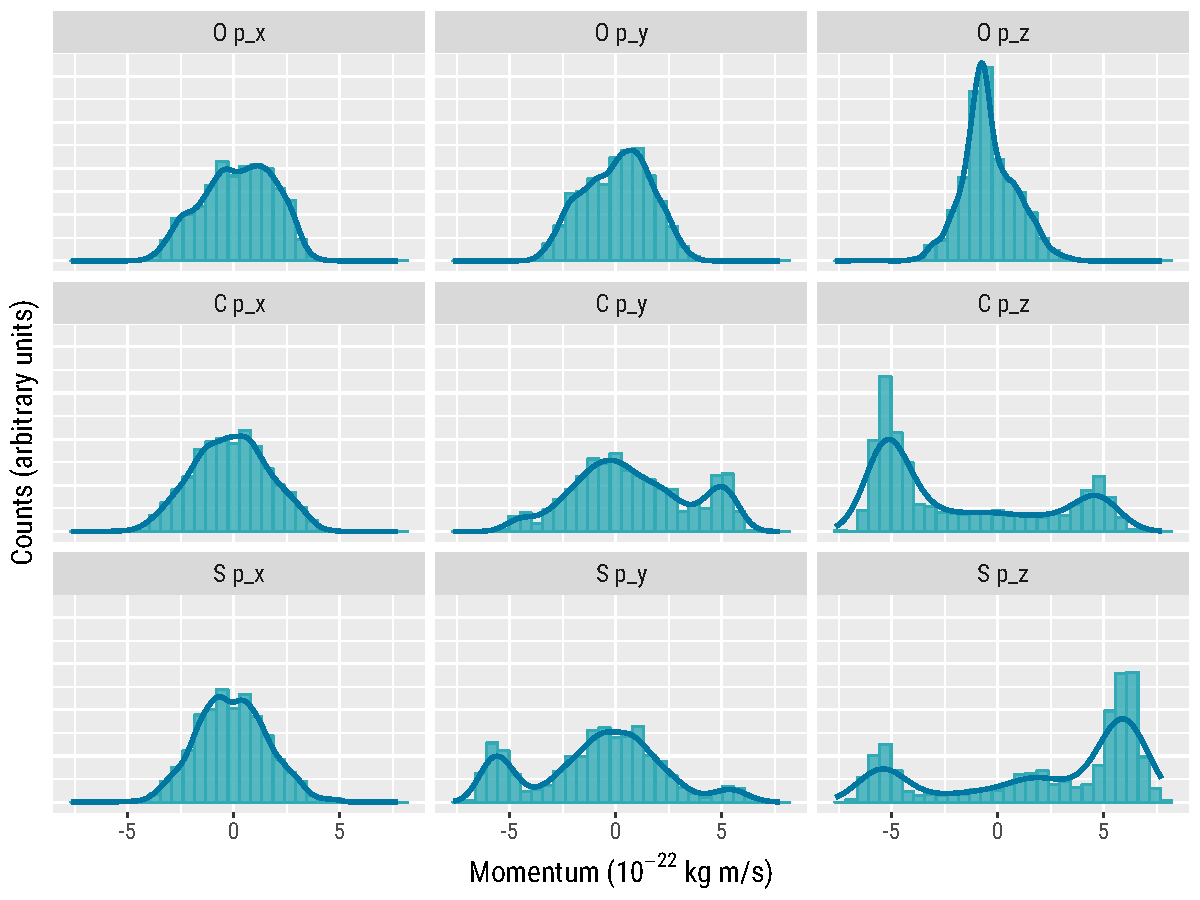
\includegraphics[width=\textwidth]{Plots/OCS22230fsMomentum}
  \caption[OCS (2,2,2) \SI{30}{\fs} momentum.]
  {OCS (2,2,2) \SI{30}{\fs} momentum.}
  \label{fig:OCS22230fsMomentum}
\end{figure}

\begin{figure}
  \centering
  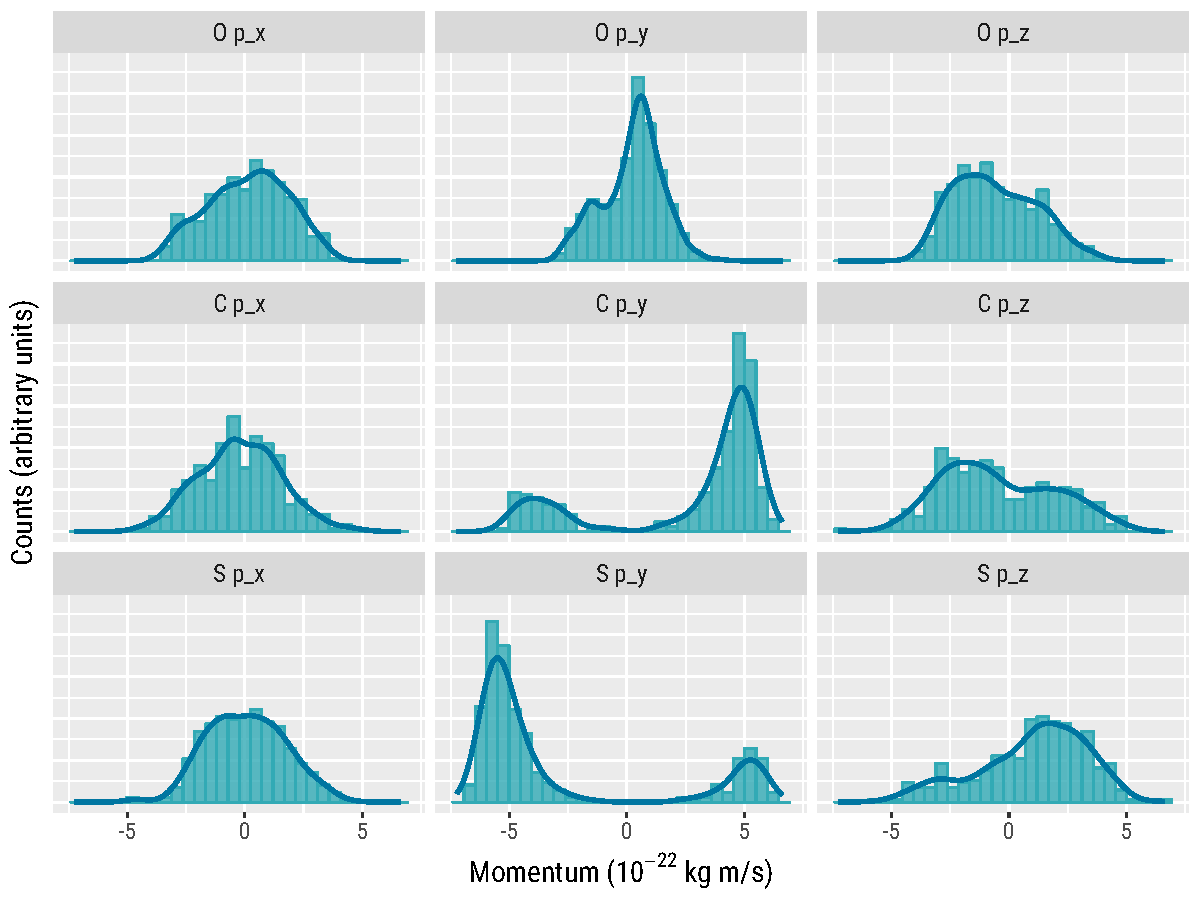
\includegraphics[width=\textwidth]{Plots/OCS22260fsMomentum}
  \caption[OCS (2,2,2) \SI{60}{\fs} momentum.]
  {OCS (2,2,2) \SI{60}{\fs} momentum.}
  \label{fig:OCS22260fsMomentum}
\end{figure}

\begin{figure}
  \centering
  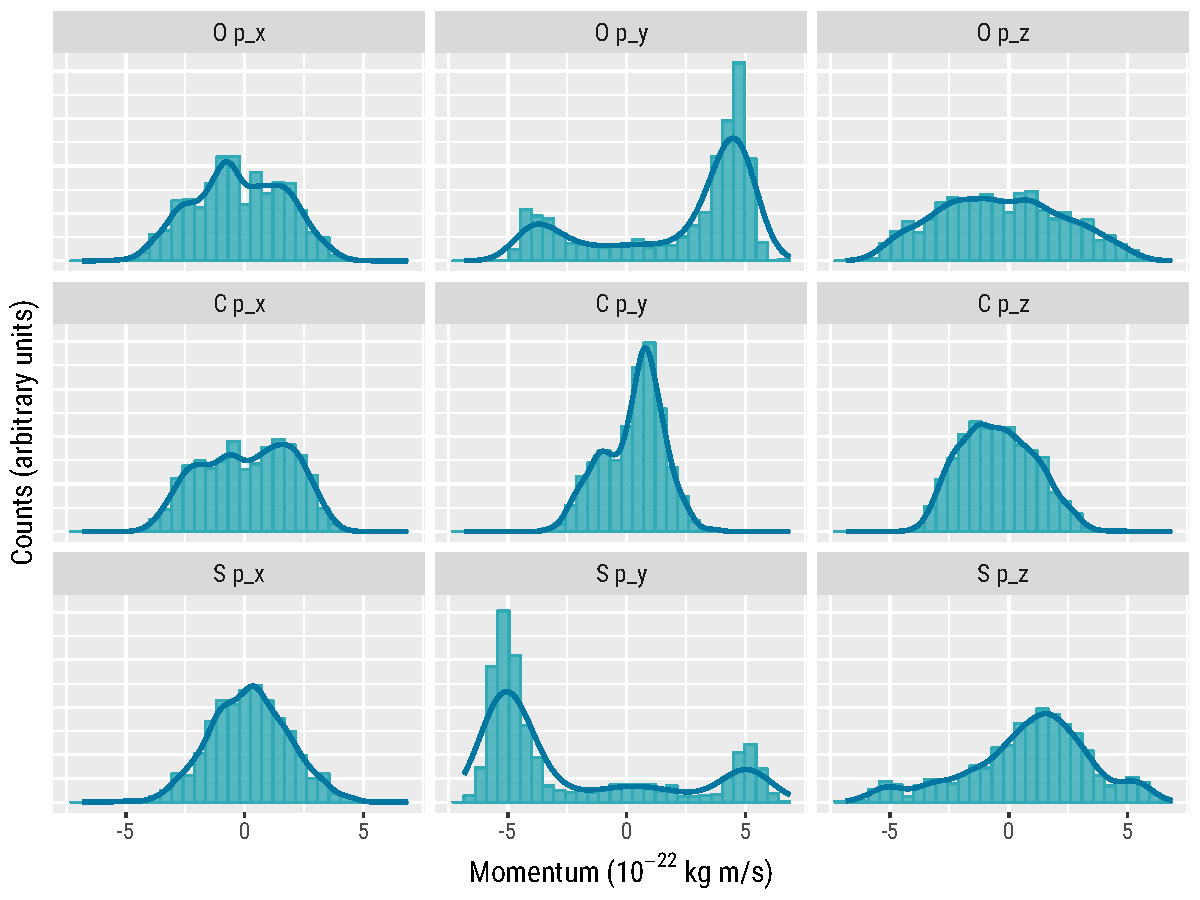
\includegraphics[width=\textwidth]{Plots/OCS222100fsMomentum}
  \caption[OCS (2,2,2) \SI{100}{\fs} momentum.]
  {OCS (2,2,2) \SI{100}{\fs} momentum.}
  \label{fig:OCS222100fsMomentum}
\end{figure}

\begin{figure}
  \centering
  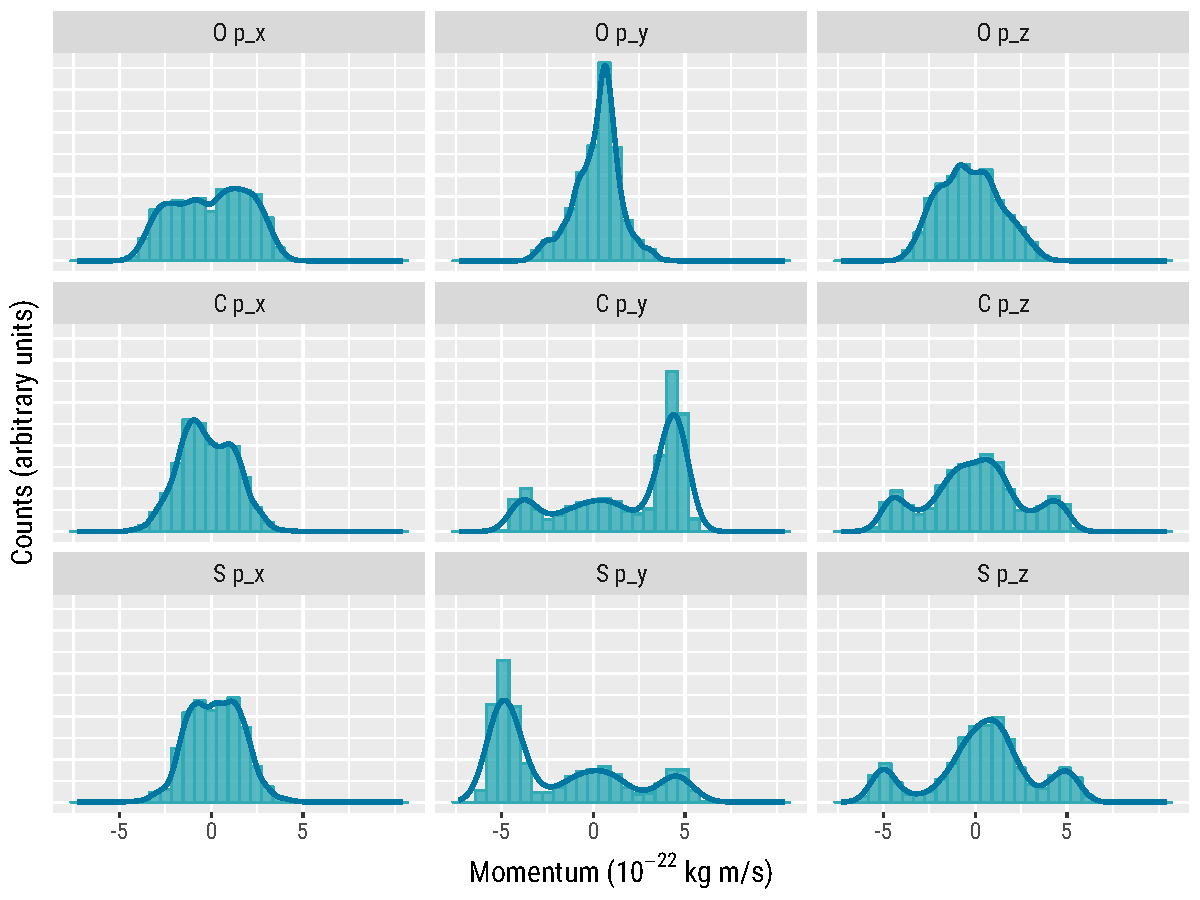
\includegraphics[width=\textwidth]{Plots/OCS222200fsMomentum}
  \caption[OCS (2,2,2) \SI{200}{\fs} momentum.]
  {OCS (2,2,2) \SI{200}{\fs} momentum.}
  \label{fig:OCS222200fsMomentum}
\end{figure}

\subsection{Momentum measurement scatter plot matrices (\SIrange{30}{200}{\femto\s})}

\begin{figure}[H]
  \centering
  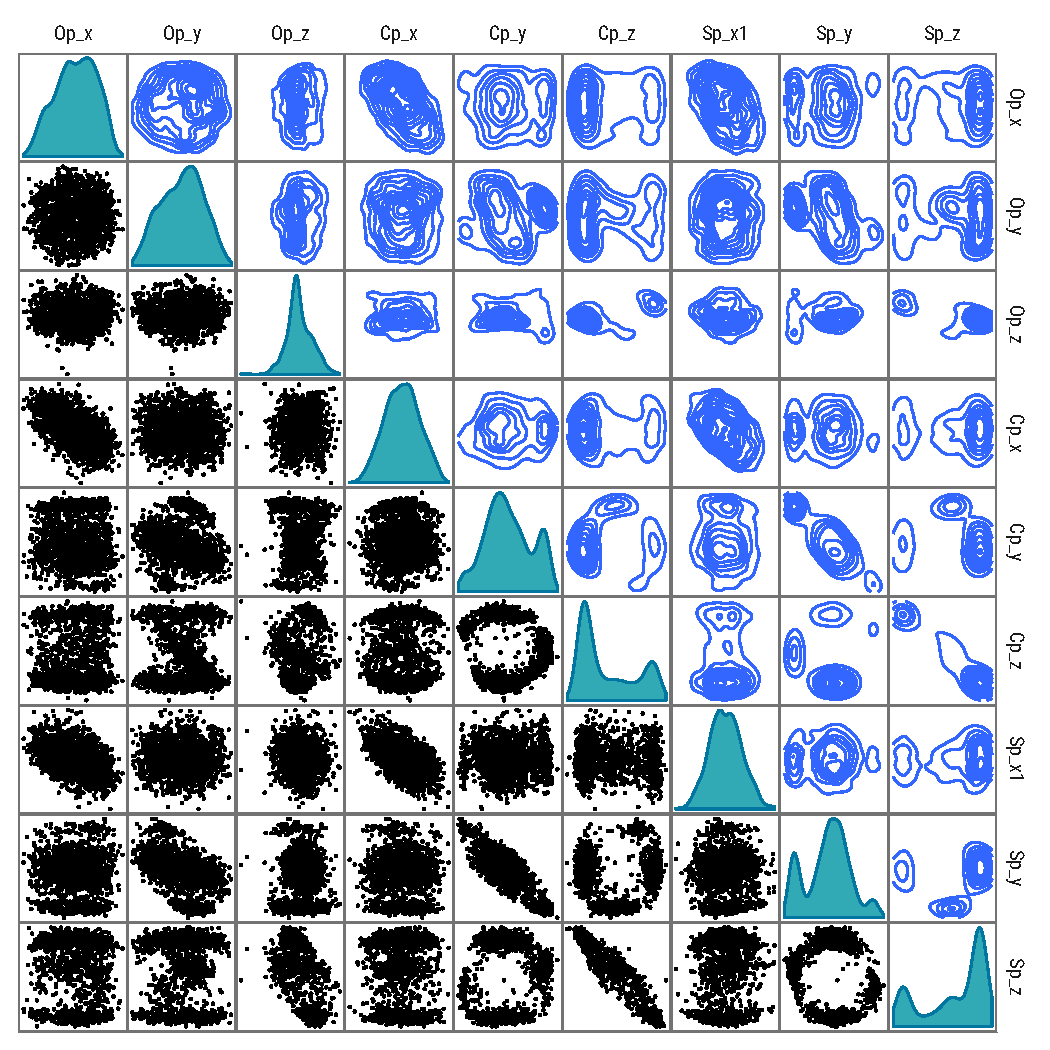
\includegraphics[width=\textwidth]{Plots/OCS22230fsMomentumPairPlots}
  \caption[OCS (2,2,2) \SI{30}{\fs} momentum pair plots.]
  {OCS (2,2,2) \SI{30}{\fs} momentum pair plots.}
  \label{fig:OCS22230fsMomentumPairPlots}
\end{figure}

\begin{figure}
  \centering
  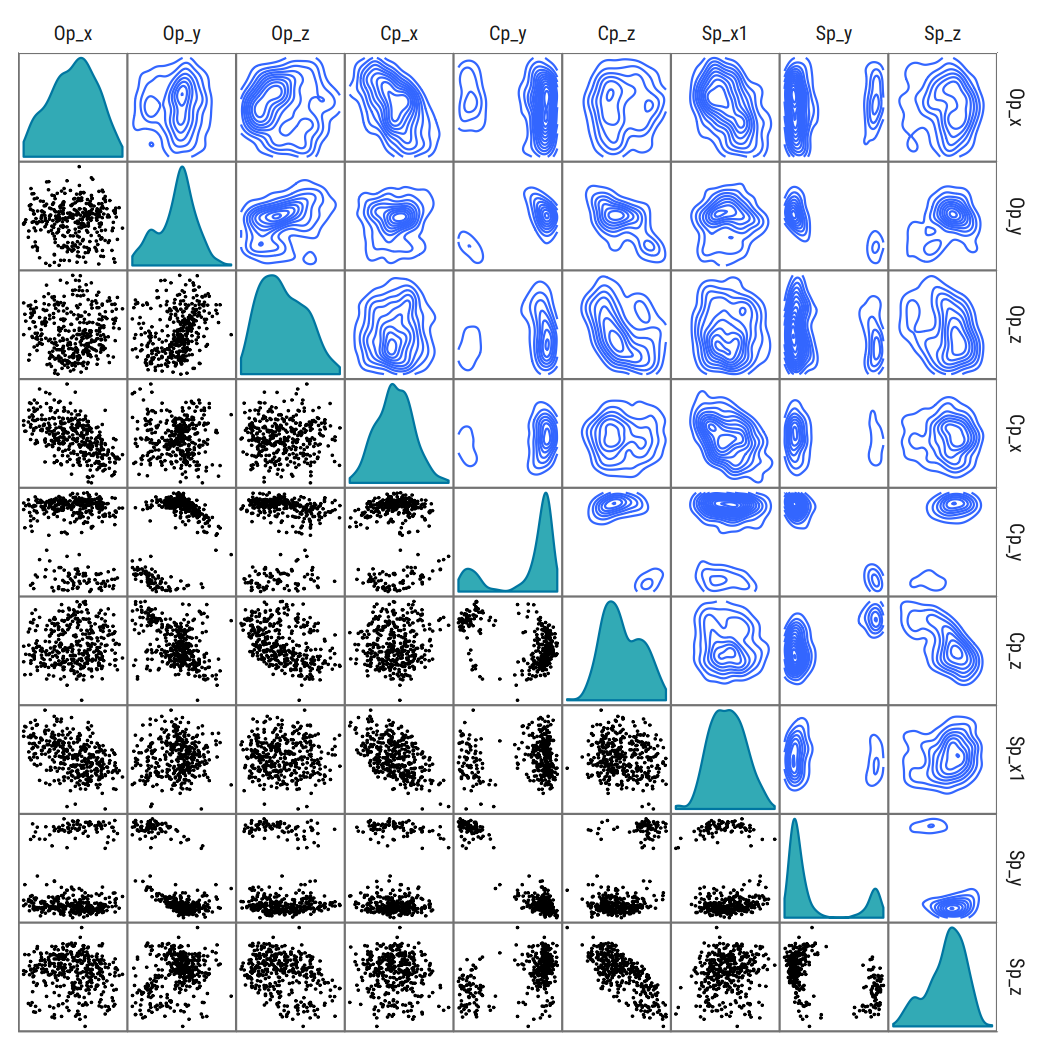
\includegraphics[width=\textwidth]{Plots/OCS22260fsMomentumPairPlots}
  \caption[OCS (2,2,2) \SI{60}{\fs} momentum pair plots.]
  {OCS (2,2,2) \SI{60}{\fs} momentum pair plots.}
  \label{fig:OCS22260fsMomentumPairPlots}
\end{figure}

\begin{figure}
  \centering
  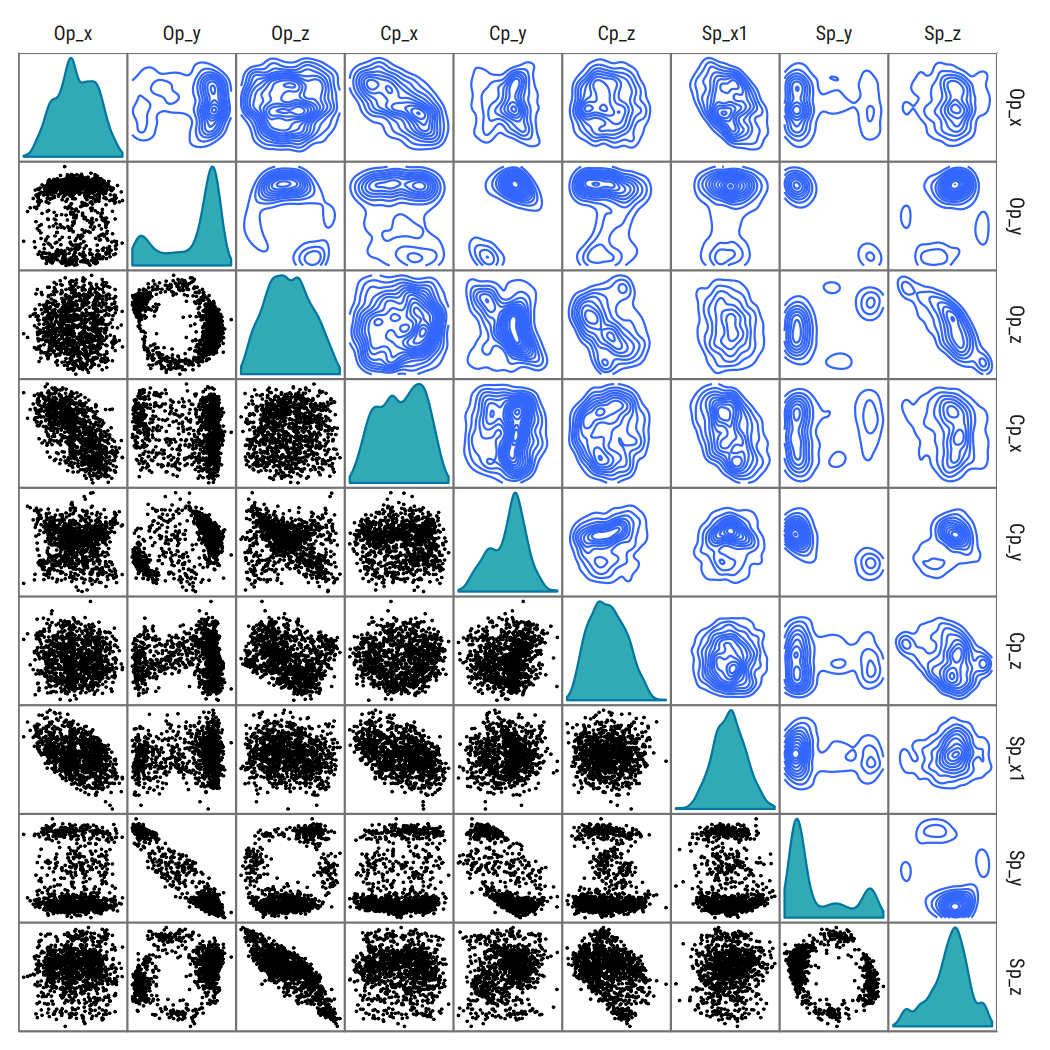
\includegraphics[width=\textwidth]{Plots/OCS222100fsMomentumPairPlots}
  \caption[OCS (2,2,2) \SI{100}{\fs} momentum pair plots.]
  {OCS (2,2,2) \SI{100}{\fs} momentum pair plots.}
  \label{fig:OCS222100fsMomentumPairPlots}
\end{figure}

\begin{figure}
  \centering
  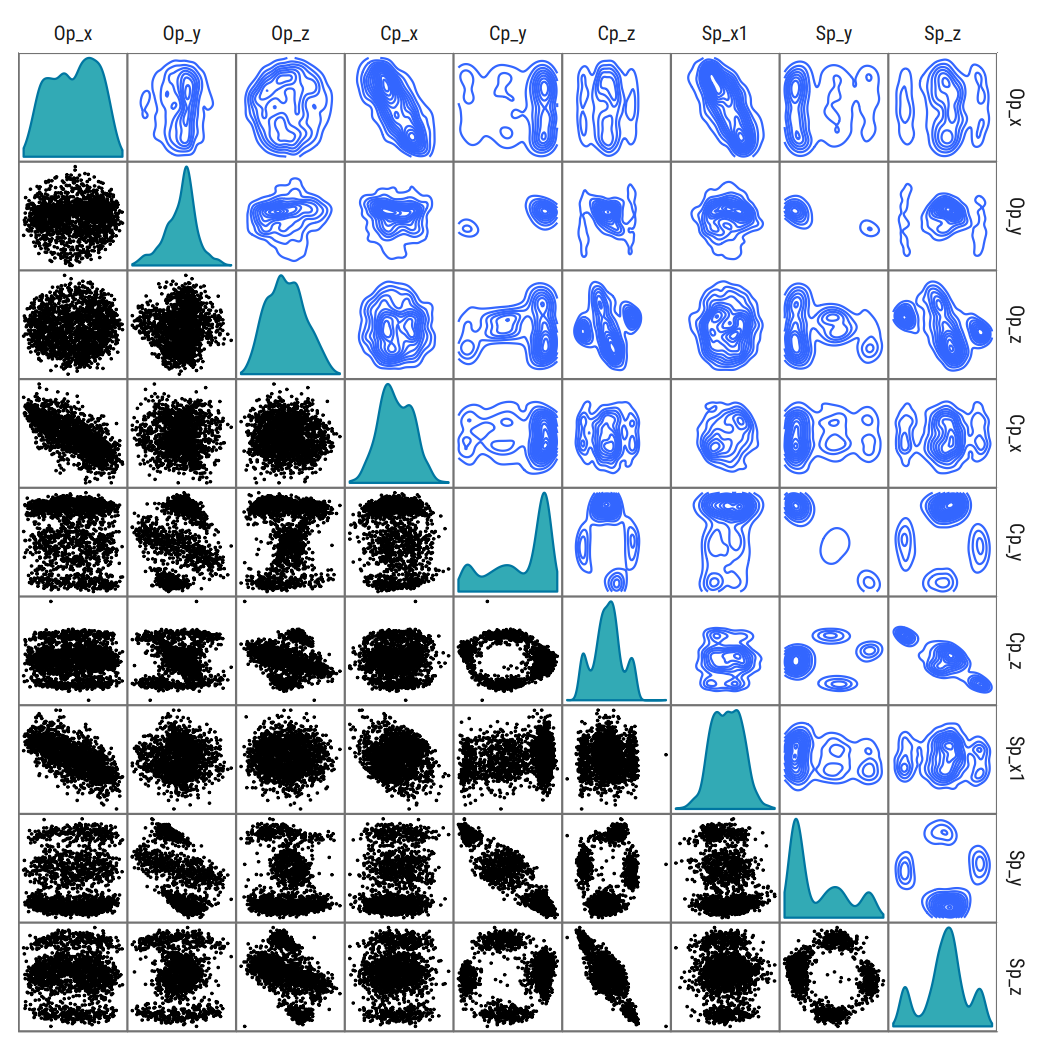
\includegraphics[width=\textwidth]{Plots/OCS222200fsMomentumPairPlots}
  \caption[OCS (2,2,2) \SI{200}{\fs} momentum pair plots.]
  {OCS (2,2,2) \SI{200}{\fs} momentum pair plots.}
  \label{fig:OCS222200fsMomentumPairPlots}
\end{figure}

\section{Lookup table geometry reconstructions}

\begin{figure}[H]
  \centering
  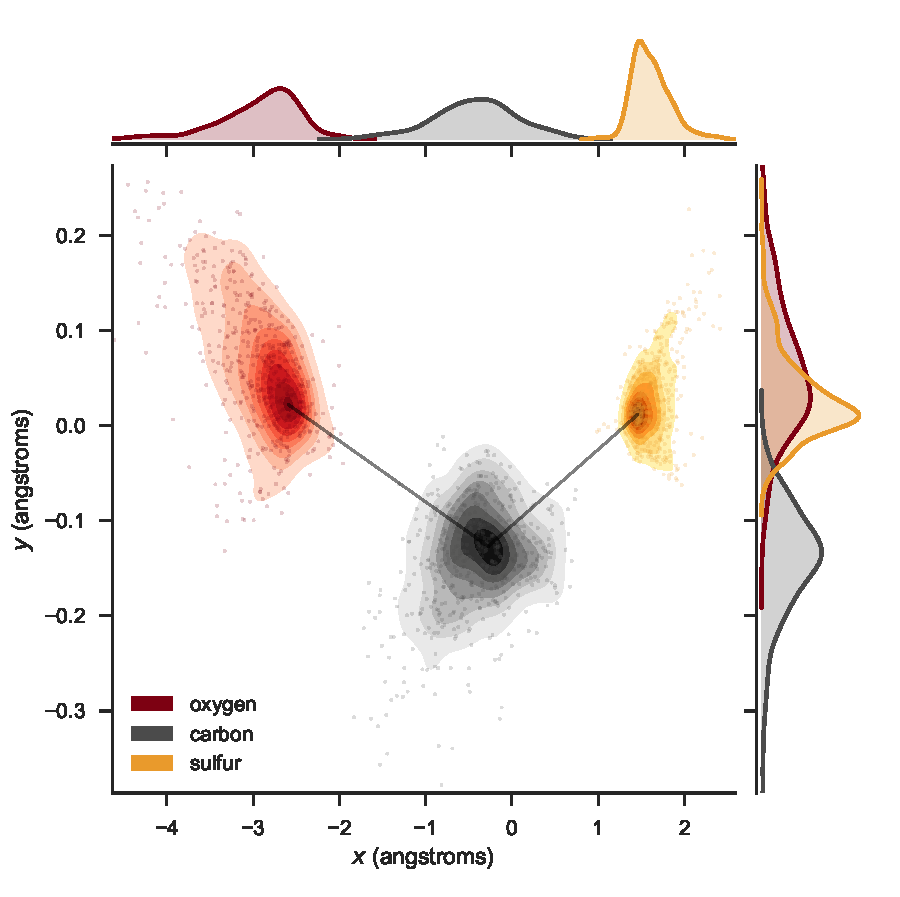
\includegraphics[width=\textwidth]{Plots/OCS22230fsLTGeometry}
  \caption[OCS (2,2,2) \SI{30}{\fs} lookup table geometry reconstruction.]
  {OCS (2,2,2) \SI{30}{\fs} lookup table geometry reconstruction.}
  \label{fig:OCS22230fsLTGeometry}
\end{figure}

\begin{figure}
  \centering
  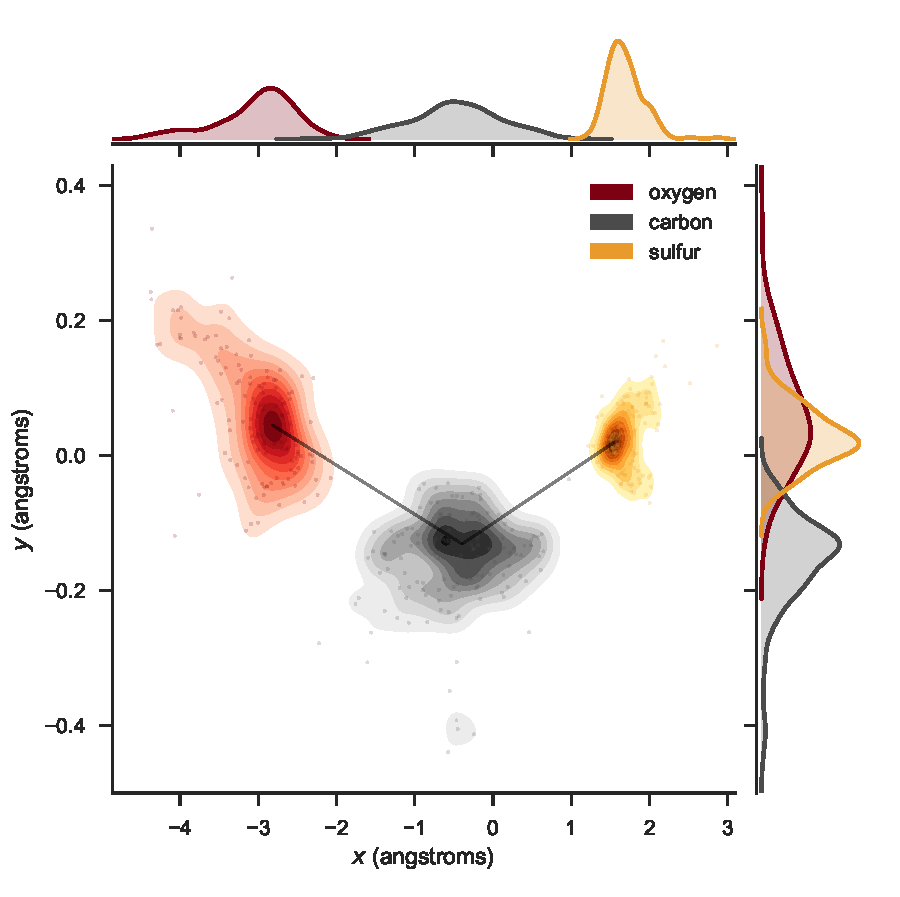
\includegraphics[width=\textwidth]{Plots/OCS22260fsLTGeometry}
  \caption[OCS (2,2,2) \SI{60}{\fs} lookup table geometry reconstruction.]
  {OCS (2,2,2) \SI{60}{\fs} lookup table geometry reconstruction.}
  \label{fig:OCS22260fsLTGeometry}
\end{figure}

\begin{figure}
  \centering
  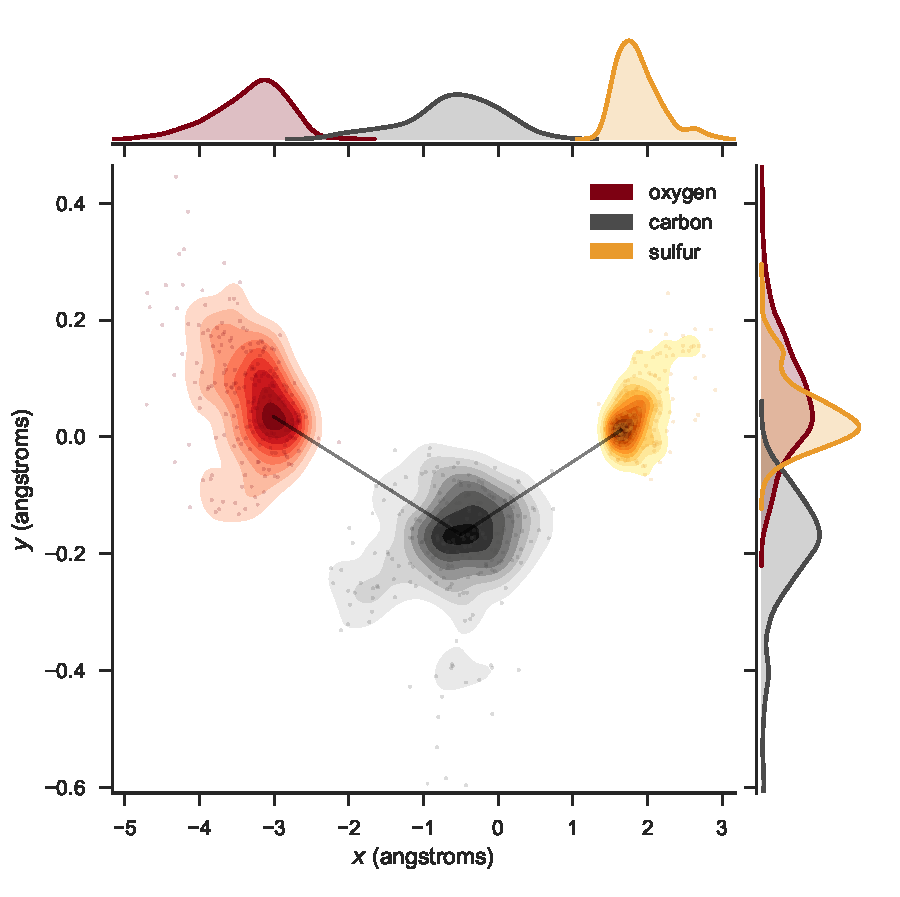
\includegraphics[width=\textwidth]{Plots/OCS222100fsLTGeometry}
  \caption[OCS (2,2,2) \SI{100}{\fs} lookup table geometry reconstruction.]
  {OCS (2,2,2) \SI{100}{\fs} lookup table geometry reconstruction.}
  \label{fig:OCS222100fsLTGeometry}
\end{figure}

\begin{figure}
  \centering
  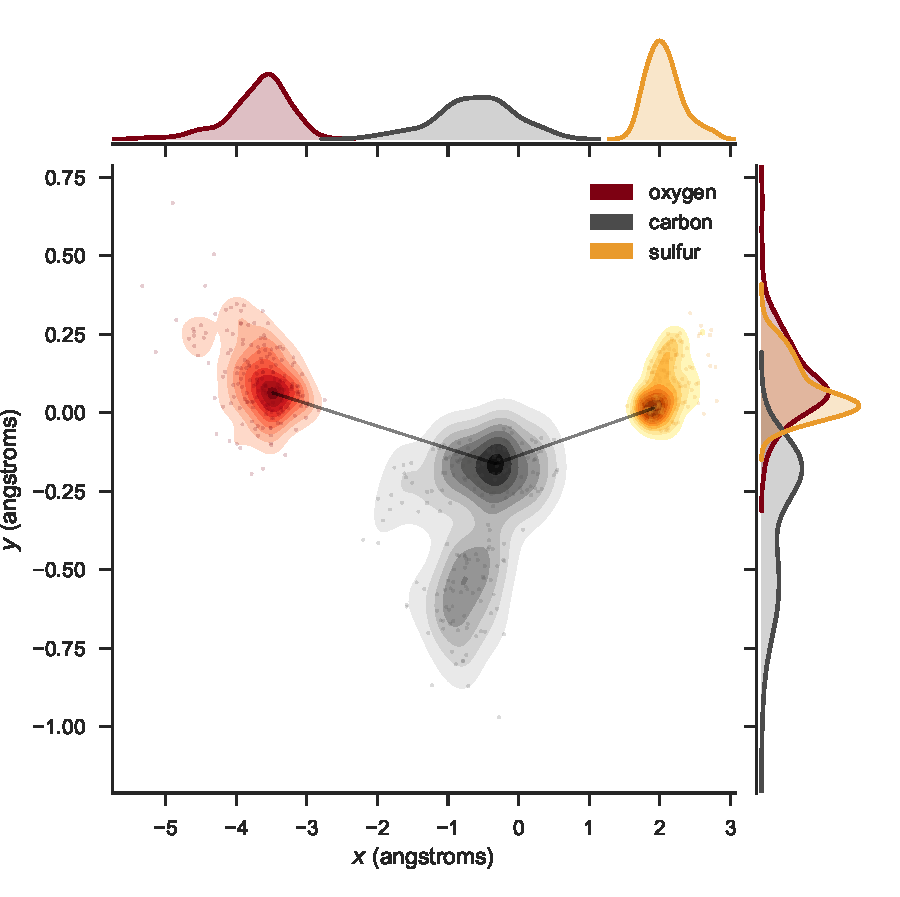
\includegraphics[width=\textwidth]{Plots/OCS222200fsLTGeometry}
  \caption[OCS (2,2,2) \SI{200}{\fs} lookup table geometry reconstruction.]
  {OCS (2,2,2) \SI{200}{\fs} lookup table geometry reconstruction.}
  \label{fig:OCS222200fsLTGeometry}
\end{figure}

\section{Mathematical optimization geometry reconstructions}

\begin{figure}[H]
  \centering
  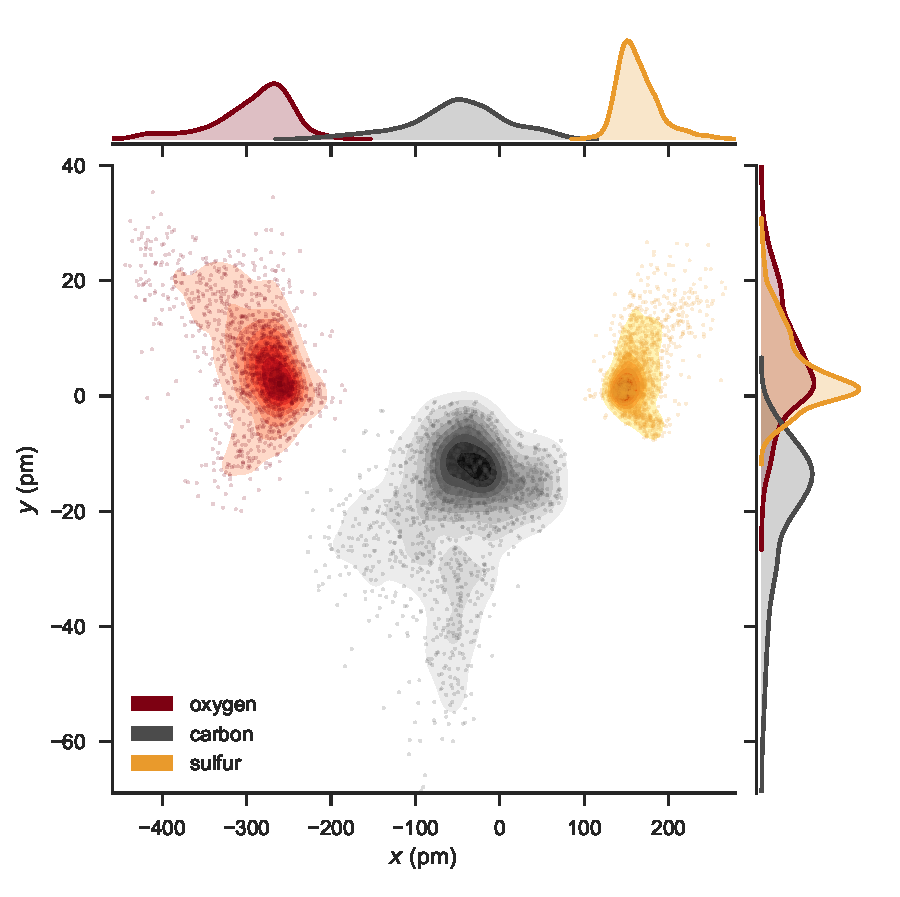
\includegraphics[width=\textwidth]{Plots/OCS22230fsMOGeometry}
  \caption[OCS (2,2,2) \SI{30}{\fs} geometry reconstructions using nonlinear constrained optimization.]
  {OCS (2,2,2) \SI{30}{\fs} geometry reconstructions using nonlinear constrained optimization.}
  \label{fig:OCS22230fsMOGeometry}
\end{figure}

\begin{figure}
  \centering
  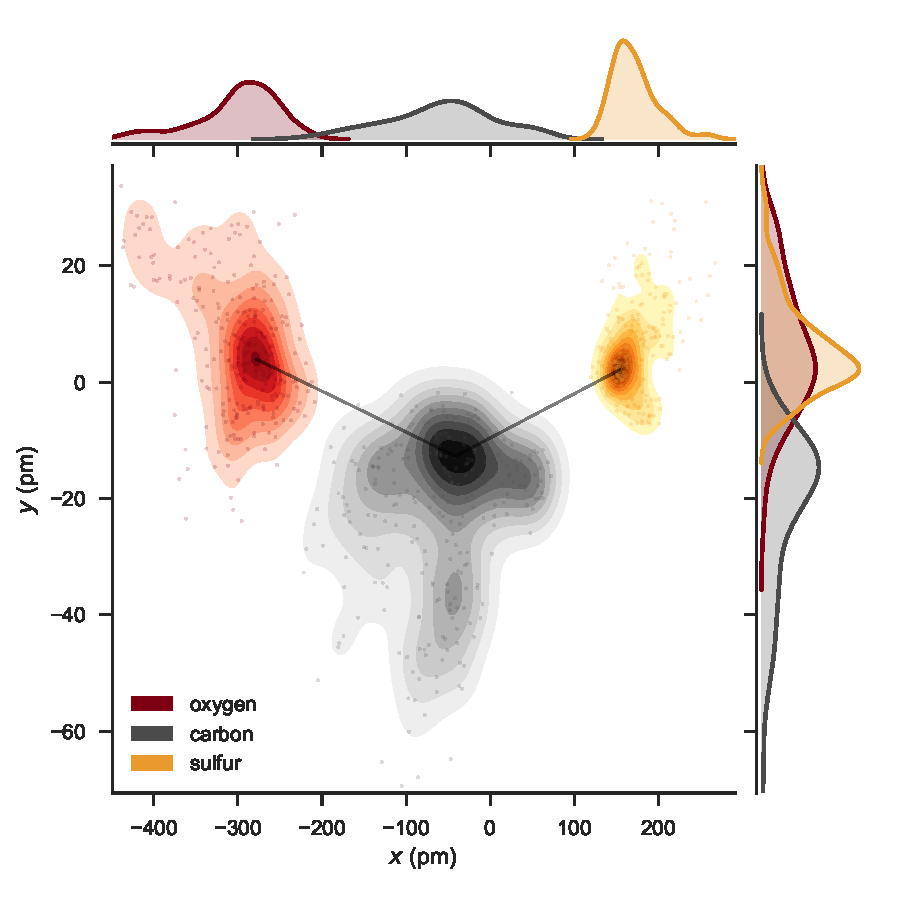
\includegraphics[width=\textwidth]{Plots/OCS22260fsMOGeometry}
  \caption[OCS (2,2,2) \SI{60}{\fs} geometry reconstructions using nonlinear constrained optimization.]
  {OCS (2,2,2) \SI{60}{\fs} geometry reconstructions using nonlinear constrained optimization.}
  \label{fig:OCS22260fsMOGeometry}
\end{figure}

\begin{figure}
  \centering
  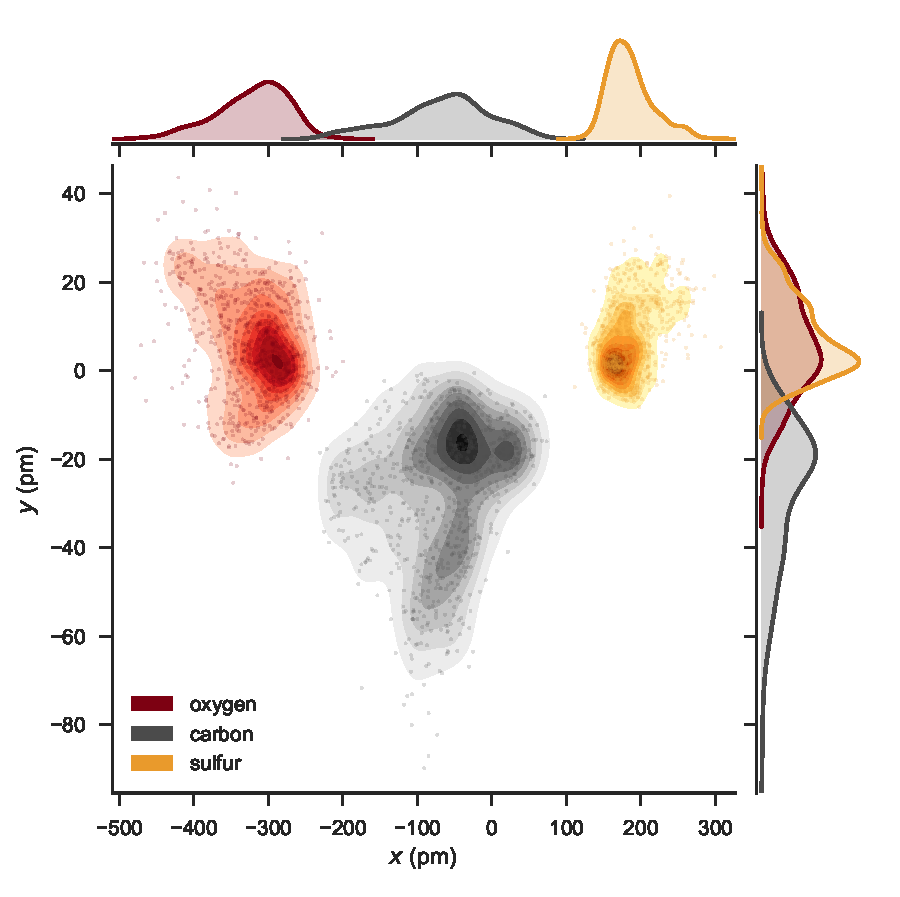
\includegraphics[width=\textwidth]{Plots/OCS222100fsMOGeometry}
  \caption[OCS (2,2,2) \SI{100}{\fs} geometry reconstructions using nonlinear constrained optimization.]
  {OCS (2,2,2) \SI{100}{\fs} geometry reconstructions using nonlinear constrained optimization.}
  \label{fig:OCS222100fsMOGeometry}
\end{figure}
\chapter{Code listings} \label{appx:code}
\chapter{Colophon} \label{appx:colophon}
\markboth{\spacedlowsmallcaps{C Colophon}}{\spacedlowsmallcaps{C Colophon}}

This document was typeset using the typographical look-and-feel \texttt{classicthesis} developed by Andr\'e Miede.
The style was inspired by Robert Bringhurst's seminal book on typography ``\emph{The Elements of Typographic Style}''.

%\cleardoublepage
%\addcontentsline{toc}{chapter}{\textsc{index}}
%\printindex

\end{document}
